%% 
%% Copyright 2019-2020 Elsevier Ltd
%% 
%% This file is part of the 'CAS Bundle'.
%% --------------------------------------
%% 
%% It may be distributed under the conditions of the LaTeX Project Public
%% License, either version 1.2 of this license or (at your option) any
%% later version. The latest version of this license is in
%%    http://www.latex-project.org/lppl.txt
%% and version 1.2 or later is part of all distributions of LaTeX
%% version 1999/12/01 or later.
%% 
%% The list of all files belonging to the 'CAS Bundle' is
%% given in the file `manifest.txt'.
%% 
%% Template article for cas-dc documentclass for 
%% double column output.

%\documentclass[a4paper,fleqn,longmktitle]{cas-dc}
\documentclass[a4paper,fleqn]{cas-dc}

% \usepackage[authoryear,longnamesfirst]{natbib}
%\usepackage[authoryear]{natbib}
\usepackage[numbers,sort&compress]{natbib}

\usepackage{algorithm}
\usepackage{algpseudocode}
\renewcommand{\algorithmicrequire}{\textbf{Input:}}  % Use Input in the format of Algorithm  
\renewcommand{\algorithmicensure}{\textbf{Output:}} % Use Output in the format of Algorithm 

\usepackage{threeparttable}%表格下面加标注
\usepackage{algpseudocode}
\usepackage{threeparttable}%表格下面加标注

% Attempt to fix the \pdf@box issue: load graphicx with pdftex driver and color
%\usepackage[pdftex]{graphicx}
%\usepackage{color}

% Now load hyperref (also with pdftex driver to be consistent? Actually, hyperref will use the driver automatically)
%\usepackage{hyperref}
\usepackage{float}
\usepackage{array, longtable, tabularx}
%\usepackage{caption}

\usepackage{cleveref} % 确保 cleveref 已加载
\crefname{figure}{}{}% 设置 \cref 对 figure 的引用格式为空(只留编号)
\Crefname{figure}{}{}% 设置 \Cref 对 figure 的引用格式为空(只留编号)
\crefname{table}{}{}% 设置 \cref 对 figure 的引用格式为空(只留编号)
\Crefname{table}{}{}% 设置 \Cref 对 figure 的引用格式为空(只留编号)
\crefname{section}{}{}% 设置 \cref 对 figure 的引用格式为空(只留编号)
\Crefname{section}{}{}% 设置 \Cref 对 figure 的引用格式为空(只留编号)
\usepackage{float}
\usepackage{array, longtable, tabularx}

\sloppy
%%%Author definitions
\def\tsc#1{\csdef{#1}{\textsc{\lowercase{#1}}\xspace}}
\tsc{WGM}
\tsc{QE}
\tsc{EP}
\tsc{PMS}
\tsc{BEC}
\tsc{DE}
%%% 

\begin{document}
\let\ref\Cref 		
\let\eqref\Cref 	
\let\autoref\Cref 	
\let\WriteBookmarks\relax
\def\floatpagepagefraction{1}
\def\textpagefraction{.001}
\shorttitle{Journal of Engineering Research xx (20xx) xxxxxx}
\shortauthors{Author 1 and N.S. Ahmad}
\footmarks{\url{https://doi.org/10.1016/j.jer.20xx.xx.xxx}\\
    0952-1976/\begingroup\tiny{©}\endgroup~2025 Elsevier B.V.\\
    This is an open access article under the CC BY-NC-ND license (\url{http://creativecommons.org/licenses/by-nc-nd/4.0/}).
}


% \bookmark[named = FirstPage]{A Comprehensive Survey on UWB-Based NLOS Identification and Ranging Error Mitigation Using CIR Features and Raw Sequences} % Title bookmark used in the pdf
%**************** If the title is short, stay on the first line use [mode = short_title] otherwise ******************
%***************************************** use [mode = title] below ***************************************
\title [mode = title]{Advances in Autonomous Fruit-Picking Robots: Methodologies, Technologies, and Challenges}    

% Title mark notes if desired
%\tnotemark[1,2]

%\tnotetext[1]{This document is the results of the research
%   project funded by the National Science Foundation.}

%\tnotetext[2]{The second title footnote which is a longer text matter
%   to fill through the whole text width and overflow into
%   another line in the footnotes area of the first page.}

\author[1,2]{Zhihao Zhao}[type=author, 
                        auid=000,bioid=1,
                        ]
% \ead{wangshoude@usm.my}
\credit{Conceptualization of this study, Methodology}

\address[1]{School of Electrical and Electronic Engineering, Universiti Sains Malaysia, 14300 Nibong Tebal, Penang, Malaysia}

\author[3]{Yanxiang Zhao}
\author[1]{Nur Syazreen Ahmad}[type=author, 
                        auid=001,bioid=2,
                        orcid=0000-0001-7511-2910
                        ]
%\fnmark[1]
\cormark[1]
% \ead{syazreen@usm.my}
\credit{Data curation, Writing-Original draft preparation}

\address[2]{YanTai Engineering and Technology College, 264006 YanTai, Shandong, China}
\address[3]{Central South University, Changsha, Hunan, 410083, China}
% \author[1,3]{CV Radhakrishnan}[type=editor, 
%                         auid=000,bioid=1,
%                         prefix=Sir,
%                         %role=Researcher,
%                         %orcid=0000-0001-7511-2910
%                         ]
% \cormark[1]
% %\fnmark[1]								% URL related footnote marking
% \ead{cvr_1@tug.org.in}
% %\ead[url]{www.cvr.cc, cvr@sayahna.org} % Author URL 

% \credit{Conceptualization of this study, Methodology, Software}

% \address[1]{Elsevier B.V., Radarweg 29, 1043 NX Amsterdam, The Netherlands}

% \author[2,3]{Han Theh Thanh}[style=chinese]

% \author[2,3]{CV Rajagopal}[
%    %role=Co-ordinator,
%    suffix=Jr,
%    ]
% %\fnmark[2]								% URL related footnote marking
% \ead{cvr3@sayahna.org}
% %\ead[URL]{www.sayahna.org}				% Author URL

% \credit{Data curation, Writing - Original draft preparation}

% \address[2]{Sayahna Foundation, Jagathy, Trivandrum 695014, India}

% \author
% [1,3]
% {Rishi T.} % If the author's name hits "Check for updates" button, use \\ at the break point of his/her name like {\\Rishi T.} or {First Middle\\ Lastname}
% % NOTE: Compile first without \\ then the proper separation again afterwards !!! (Not doing so, results unwanted footnote and Credit authorship contribution at the very end with \credit command if used.)
% \cormark[2]
% %\fnmark[1,3]							% URL related footnote marking
% \ead{rishi@stmdocs.in}
% %\ead[URL]{www.stmdocs.in}				% Author URL

% \address[3]{STM Document Engineering Pvt Ltd., Mepukada,
%     Malayinkil, Trivandrum 695571, India}

% \author[4]{ \\Salih Baris Ozturk} % Author's name hits "Check for updates" button, \\ is used at the break point of his name. If \\ is desired at the beginning of the name, place a space just before the \\ as in the above example.
% % NOTE: Compile first without \\ and the space, then the proper separation again afterwards !!! (Not doing so, results unwanted footnote and Credit authorship contribution at the very end with \credit command if used.)
% %\cormark[1]
% \ead{ozturksb@itu.edu.tr}

% \address[4]{Istanbul Technical University, Department of Electrical Engineering,
% 	Maslak, Istanbul 34469, Turkey}

\credit{Modification for the final layout}

\cortext[1]{Corresponding author.}
% \cortext[cor2]{Principal corresponding author.}
% \fntext[1]{E-mail address: \href{mailto:syazreen@usm.my}{syazreen@usm.my} (N.S. Ahmad).}
%\fntext[fn2]{Another author footnote, this is a very long footnote and
%  it should be a really long footnote. But this footnote is not yet
%  sufficiently long enough to make two lines of footnote text.}

%\nonumnote{This note has no numbers. In this work we demonstrate $a_b$
%  the formation Y\_1 of a new type of polariton on the interface
%  between a cuprous oxide slab and a polystyrene micro-sphere placed
%  on the slab. The evanescent field of the resonant whispering 
%  gallery mode (\WGM) of the micro sphere has a substantial 
%  gradient, and therefore effectively couples with the
%  quadrupole $1S$ excitons in cuprous oxide.}

\nonumnote{E-mail address: \href{mailto:syazreen@usm.my}{syazreen@usm.my} (N.S. Ahmad).}

\begin{abstract} 
The advent of autonomous fruit-picking robots has precipitated a paradigm shift in contemporary agriculture, with the potential to address the prevailing labour shortage and enhance harvesting efficiency. This review comprehensively surveys recent progress in fruit-picking robotics, focusing on vision-based detection, learning-based strategies, arm motion planning, and collision avoidance. Employing a Preferred Reporting Items for Systematic Reviews and Meta-Analyses (PRISMA)-based systematic methodology, over 130 influential studies from 2015–2024 were analysed. Recent advances in vision-based detection, including multi-sensor fusion and 3D data acquisition, have enhanced robots' ability to localise and identify fruits under complex agricultural conditions. The efficacy of deep learning (DL) models, such as the Regions with Convolutional Neural Networks (R-CNN) and You Only Look Once (YOLO) series, has been demonstrated in enhancing real-time detection performance, particularly in scenarios where there is occlusion and variable lighting. It is evident that learning-based approaches, including transfer learning and reinforcement learning (e.g., Deep Deterministic Policy Gradient (DDPG)), have enhanced the generalisation capabilities and optimised the robotic arm motion planning for collision-free harvesting. Innovative path-planning algorithms and robust control strategies further enable autonomous robots to navigate unstructured environments and compensate for real-time disturbances, increasing system reliability. Notwithstanding these advances, challenges persist in guaranteeing precise multi-source data integration, delicate fruit handling, and robust operation across diverse and unpredictable environments. The paper highlights trends towards the integration of the Internet of Things (IoT), advanced sensors, and machine learning (ML). It identifies research gaps in scalability and real-world deployment, and proposes future research directions. This survey provides a comprehensive and critical evaluation of technological advancements and ongoing challenges in the field of autonomous fruit-picking robotics. The primary objective of the survey is to provide a foundation for guiding future research and accelerating the commercial adoption of these transformative systems.

\end{abstract}

% If any graphical abstract is needed
%\begin{graphicalabstract}
%\includegraphics{figs/grabs.pdf}
%\end{graphicalabstract}

% If any highlights is needed above the cover page
%\begin{highlights}
%\item Research highlights item 1
%\item Research highlights item 2
%\item Research highlights item 3
%\end{highlights}

% Article history - Should only be set by an editor
\received {xx Month 20xx}
\revised {xx Month 20xx}
\accepted {xx Month 20xx}
\online {xx Month 20xx}

\begin{keywords}
 Autonomous Fruit-Picking Robots,
Regions with Convolutional Neural Networks (R-CNN),
You Only Look Once (YOLO),
Motion Planning,
Transfer Learning.
\end{keywords}

\maketitle

\section{Introduction}
Rapid advancements in robotics and artificial intelligence have catalyzed substantial interest in developing fruit-picking robots. These robots promise to revolutionize agricultural practices by automating labor-intensive fruit harvesting. 
Fruit-picking robots are autonomous systems engineered to identify, locate, and harvest fruits from various trees and plants. These systems leverage a suite of advanced technologies, including computer vision, machine learning (ML), robotics, and Internet of Things (IoT). The aim is to create robots that can operate efficiently in various agricultural environments, handle fruits delicately to avoid damage, and work alongside human labor to enhance productivity. 
%like Figure~\ref{fig:fruit_picking_robot_overview}.

Previous reviews synthesize the latest research trends across multiple interconnected aspects as illustrated in Table~\ref{tab:survey_summary}, ranging from data acquisition to model optimization and motion control. These advancements are pivotal in enhancing operational efficiency in unstructured agricultural environments, with a consistent focus on addressing core challenges such as variable field conditions and complex fruit-picking tasks. Key technological progress includes multi-sensor fusion (e.g., IoT and remote sensing integration \cite{mohamed2021smart,friha2021internet,martos2021ensuring}), advanced visual models (e.g., MTA-YOLACT for precise segmentation \cite{li2023mta}), and collaborative robotics (e.g., multi-arm coordination \cite{lytridis2021overview,li2023multi}), all of which contribute to scaled-up and efficient picking operations.

Data acquisition forms the foundation of smart fruit-picking systems. Integrated IoT and remote sensing (RS) technologies have revolutionized crop monitoring: IoT-enabled sensors provide real-time data on fruit ripeness and environmental conditions \cite{mohamed2021smart,friha2021internet}, while satellite and UAV-based RS offer broad-scale insights into crop health and yield \cite{martos2021ensuring}. This multi-scale data integration enables proactive decision-making, from targeted harvesting schedules to disease intervention, laying the groundwork for precise robotic operations.
Building on this data foundation, visual models have advanced significantly in enhancing robotic perception. Hou et al. \cite{hou2023overview} highlight how machine vision and ML enable fruit defect detection, ripeness assessment, and health monitoring, while Suresh et al. \cite{suresh2023selective} compare traditional and DL methods to address challenges like variable lighting and occlusion. Notably, Li et al. \cite{li2023mta}’s MTA-YOLACT model achieves accurate identification of fruit bunches, pedicels, and stems, directly supporting end-effector motion planning—critical for minimizing fruit damage during picking.

Motion planning and control systems have evolved to complement these perceptual advancements. Gai et al. \cite{gai2022fruit} emphasize efficient path planning algorithms tailored to complex orchard terrains, while Liu et al. \cite{liu2024hierarchical} integrate LiDAR-vision fusion and hierarchical trajectory planning to navigate unstructured environments. These developments ensure robots can reach target fruits safely, balancing real-time adaptability with optimal route efficiency—key for reducing cycle times in large-scale operations.
Collectively, these technologies enhance operational efficiency by enabling precise detection, collision-free navigation, and coordinated multi-robot operations \cite{li2023multi,zhang2024automatic}. However, prior reviews highlight critical limitations: visual models often lack robustness in diverse field conditions due to controlled-environment training; integration between perception and motion planning remains fragmented, limiting real-time route optimization; and dynamic environmental changes (e.g., sudden occlusion) still hinder path planner performance.

Further, while innovations like soft grippers \cite{navas2021soft} and bio-inspired systems \cite{wang2023biologically} improve mechanical efficiency and reduce labor dependency, their adaptability to diverse crops and real-world variability is limited. Darwin et al. \cite{darwin2021recognition} note that even advanced disease diagnosis and yield estimation models struggle with real-world applicability, impacting the precision of downstream picking operations. Zhang et al. \cite{zhang2024automatic} emphasize that integrating disparate technologies (e.g., vision systems with grippers) and high implementation costs remain barriers to widespread adoption, particularly for small-scale farmers. Addressing these gaps requires integrated, low-cost solutions that bridge data, perception, planning, and actuation—essential for realizing the full potential of autonomous fruit-picking robots.

\iffalse
Previous review synthesizes the latest research trends across multiple interconnected aspects as illustrated in Table~\ref{tab:survey_summary}, ranging from data management and acquisition to model development and mechanical optimization. These advanced technologies have become pivotal in enhancing operational efficiency across multiple domains. Notably, prior review efforts have consistently focused on applying cutting-edge technologies to address diverse challenges, with a particular emphasis on improving picking efficiency in unstructured real-world orchard environments. Examples of such technological advancements include multi-sensor and multi-modal sensor fusion (e.g., IoT and remote sensing integration \cite{mohamed2021smart,friha2021internet,martos2021ensuring}); optimization of model architectures (e.g., MTA-YOLACT for instance segmentation \cite{li2023mta}); and collaborative robotics (e.g., cooperative robotic systems \cite{lytridis2021overview,li2023multi}), which facilitates scaled-up picking operations.
In the context of fruit picking, data acquisition is fundamental to the advancement of smart agricultural technologies. Recent research has explored emerging technologies and the necessity of standardized datasets, aiming to enhance the efficiency and reliability of fruit-picking operations. The integration of IoT and remote sensing (RS) has transformed data collection in fruit orchards. Mohamed et al. \cite{mohamed2021smart}, Friha et al. \cite{friha2021internet}, and Martos et al. \cite{martos2021ensuring} have shown that IoT-enabled sensors, ranging from basic environmental monitors to advanced fruit-ripeness detectors, provide essential data for crop management, while satellite and UAV-based RS offers broad-scale insights into crop health, yield estimation, and disease detection. For instance, multi-spectral and hyperspectral imagery can identify early signs of nutrient deficiencies or diseases, enabling proactive interventions. Such data-driven approaches lay the foundation for precise and efficient fruit-picking operations, bridging the gap between traditional farming and smart agriculture.
In the domain of visual models for fruit picking, significant progress has been made to enhance agricultural robots’ perception capabilities. Hou et al. \cite{hou2023overview} highlight the integration of machine vision and ML in crop inspection and yield prediction, showing that vision systems leveraging feature extraction and classification algorithms can detect fruit defects, assess ripeness, and monitor crop health. However, real-world challenges like variable lighting, complex backgrounds, and overlapping fruits often degrade model performance, limiting their generalization in unstructured fields. Suresh et al. \cite{suresh2023selective} address these issues through comparative analysis of traditional and DL vision methods, while Li et al. \cite{li2023mta} propose MTA-YOLACT to achieve accurate identification of fruit bunches, pedicels, and main stems, providing precise visual support for end-effector motion planning. These advancements in visual perception directly contribute to the reliability of fruit detection, a critical prerequisite for successful robotic harvesting.
For path planning, Gai et al. \cite{gai2022fruit} emphasize the critical role of localization, mapping, and algorithm efficiency. While indoor path planning principles offer foundational insights, outdoor applications must address dynamic obstacles, uneven terrain, and changing crop layouts. Current algorithms focus on efficient and safe movement path planning in complex orchard environments, though balancing real-time adaptability with optimal route planning remains a challenge, leading to inefficiencies in robotic operations. Liu et al. \cite{liu2024hierarchical} further advance this by integrating LiDAR-vision fusion and hierarchical trajectory planning to navigate unstructured terrain. The synergy between robust visual perception and optimized path planning ensures that robots can reach target fruits while avoiding obstacles, a key factor in improving harvesting efficiency.
Collectively, these studies reveal key limitations. Firstly, visual models lack robustness in diverse field conditions due to controlled-environment training; secondly, integration between vision systems and path planning remains fragmented, failing to optimize picking routes with real-time fruit location data; finally, path planners struggle with dynamic environmental changes, hindering operational efficiency. Bridging these gaps requires interdisciplinary innovation to develop adaptive, integrated solutions for intelligent fruit picking.
A series of reviews have documented the significant impact of these innovations on agricultural productivity, spanning disease diagnosis, yield estimation, robotic operations, and mechanical harvesting. For disease diagnosis and yield estimation, Darwin et al. \cite{darwin2021recognition} highlight the transformative potential of machine vision, AI, and DL models, enabling timely management decisions by automating plant disease detection and crop yield estimation. However, their effectiveness in real-world, variable agricultural environments remains a challenge, which directly affects the precision of fruit-picking robots that rely on such data.
In the realm of robotics, Lytridis et al. \cite{lytridis2021overview} explore advancements in cooperative robotics and automation, with systems such as mobile cotton-harvesting robots replacing manual labor, improving resource utilization and operational speed. Li et al. \cite{li2023multi} develop multi-arm coordination systems to enhance throughput via coordinated motion, addressing low single-arm efficiency and collision risks. Yet, ensuring seamless coordination among robots and adapting to dynamic field conditions remain ongoing challenges, which are particularly pronounced in dense orchard settings where fruit-picking robots operate.
Regarding mechanical performance, Navas et al. \cite{navas2021soft} underscore the role of innovative designs (e.g., soft grippers) in boosting harvesting efficiency, minimizing crop damage during collection. Wang et al. \cite{wang2023biologically} propose biologically inspired solutions, such as conditional GAN and stereo vision combined with brain-inspired motion control, to address labor shortages and difficult picking in vertical growing environments. However, the adaptability of these tools to diverse crop types and environmental variations still requires improvement, limiting their widespread application in fruit picking.
Despite these achievements, existing technological applications face notable limitations. Many advanced models and robotic systems are developed under controlled conditions, leading to performance degradation in real-world, unstructured fields. Integrating disparate technologies, such as combining vision systems with robotic grippers or coordinating multiple robots, remains a complex task, as noted by Zhang et al. \cite{zhang2024automatic}. Additionally, the high cost of implementation poses a significant barrier for small-scale farmers, hindering widespread adoption. Addressing these issues is crucial for further enhancing agricultural efficiency and promoting sustainable farming practices, ensuring that fruit-picking robots can fulfill their potential in transforming agriculture.
\fi
\iffalse
%In recent years, the agricultural sector has witnessed a remarkable transformation driven by technological advancements, particularly in the domains of smart agriculture and precision farming. 
Previous review synthesizes the latest research trends across multiple interconnected aspects as illustrated in Table~\ref{tab:survey_summary}, ranging from data management and acquisition to model development and mechanical optimization. These advanced technologies have become pivotal in enhancing operational efficiency across multiple domains. Notably, prior review efforts have consistently focused on applying cutting-edge technologies to address diverse challenges, with a particular emphasis on improving picking efficiency in unstructured real-world orchard environments. Examples of such technological advancements include multi-sensor and multi-modal sensor fusion, which enhances data perception accuracy; optimization of model architectures from two-stage to one-stage designs, which boosts the efficiency of detection and segmentation tasks; and collaborative robotics, which facilitates scaled-up picking operations.


In the context of fruit picking, data acquisition is fundamental to the advancement of smart agricultural technologies. Recent research has explored emerging technologies and the necessity of standardized datasets, aiming to enhance the efficiency and reliability of fruit-picking operations.
The integration of IoT and remote sensing (RS) has transformed data collection in fruit orchards. Mohamed et al. \cite{mohamed2021smart}, Ayaz et al. \cite{ayaz2019internet}, Friha et al. \cite{friha2021internet}, and Visconti et al. \cite{visconti2020development} have shown that IoT-enabled sensors, ranging from basic environmental monitors to advanced fruit-ripeness detectors, provide essential data for crop management. Meanwhile, studies by Khanal et al. \cite{khanal2020remote} and Martos et al. \cite{martos2021ensuring} highlight how satellite and unmanned aerial vehicles (UAV)-based RS offers broad-scale insights into crop health, yield estimation, and disease detection. For instance, multi-spectral and hyper-spectral imagery can identify early signs of nutrient deficiencies or diseases, enabling proactive interventions.
Data security in fruit-picking operations has also gained attention. Pranto et al. \cite{pranto2021blockchain} proposed blockchain technology as a solution to safeguard data integrity across the supply chain. Its decentralized and immutable nature reduces the risk of data tampering, ensuring transparency from production to distribution.
However, data standardization remains a significant challenge. Lu et al. \cite{lu2020survey} noted the lack of unified standards in precision agriculture datasets, causing inconsistencies in data formats and annotations. This hinders the development of reliable fruit-picking algorithms. Luo et al. \cite{luo2020identifying} emphasized the need for high-resolution, time-continuous data to accurately map fruit growth and optimize harvesting schedules.
Despite these advancements, existing research has limitations. The integration of IoT and RS data is complicated by differences in data formats and collection frequencies. Implementing blockchain in real-world agriculture faces barriers such as high costs and technical complexity. Additionally, establishing comprehensive data standards and acquiring high-precision, continuous datasets require collaborative efforts and technological innovation.

In the domain of visual models for fruit picking, significant progress has been made to enhance agricultural robots' perception capabilities. Cubero et al. \cite{cubero2016automated}, Hameed et al. \cite{hameed2018comprehensive}, and Sharma et al. \cite{sharma2020machine} collectively highlight the integration of machine vision and ML in crop inspection and yield prediction. These studies show that vision systems leveraging feature extraction and classification algorithms can detect fruit defects, assess ripeness, and monitor crop health. However, real-world challenges like variable lighting, complex backgrounds, and overlapping fruits often degrade model performance, limiting their generalization in unstructured fields.
For path planning, Aguiar et al. \cite{aguiar2020localization}, Bormann et al. \cite{bormann2018indoor}, and Zhou et al. \cite{zhou2022intelligent} emphasize the critical role of localization, mapping, and algorithm efficiency. While indoor path planning principles offer foundational insights, outdoor applications must address dynamic obstacles, uneven terrain, and changing crop layouts. Current algorithms struggle to balance real-time adaptability with optimal route planning, leading to inefficiencies in robotic operations.
Collectively, these studies reveal key limitations. Firstly, visual models lack robustness in diverse field conditions due to controlled-environment training; Secondly, integration between vision systems and path planning remains fragmented, failing to optimize picking routes with real-time fruit location data; Finally, path planners struggle with dynamic environmental changes, hindering operational efficiency. Bridging these gaps requires interdisciplinary innovation to develop adaptive, integrated solutions for intelligent fruit picking.

A series of reviews have documented the significant impact of these innovations on agricultural productivity, spanning disease diagnosis, yield estimation, robotic operations, and mechanical harvesting.
For disease diagnosis and yield estimation, Ampatzidis et al. \cite{ampatzidis2017ipathology} and Darwin et al. \cite{darwin2021recognition} highlighted the transformative potential of machine vision, AI, and deep-learning models. By automating the detection of plant diseases and accurately estimating crop yields, these technologies enable timely management decisions, reducing losses and optimizing resource allocation. However, their effectiveness in real-world, variable agricultural environments remains a challenge.
In the realm of robotics, Lytridis et al. \cite{lytridis2021overview}, Aragund et al. \cite{aravind2017task}, and Fue et al. \cite{fue2020extensive} explored the advancements in robotic collaboration and automation. Cooperative robotics and task-based systems, such as mobile cotton-harvesting robots, have replaced manual labor, improving resource utilization and operational speed. Yet, ensuring seamless coordination among robots and adapting to dynamic field conditions remain ongoing challenges.
Regarding mechanical performance, research by Zhang et al. \cite{zhang2016development,zhang2020technology}, Zhang et al. \cite{zhang2020state}, Navas et al. \cite{navas2021soft}, and Jia et al. \cite{jia2020apple} underscored the role of innovative designs in boosting harvesting efficiency. Mechanical apple-harvesting technologies and robotic grippers, especially soft grippers, have minimized crop damage during collection. However, the adaptability of these tools to diverse crop types and environmental variations still requires improvement.
Despite these achievements, existing technological applications face notable limitations. Many advanced models and robotic systems are developed under controlled conditions, leading to performance degradation in real-world, unstructured fields \cite{ampatzidis2017ipathology,darwin2021recognition}. Integrating disparate technologies, such as combining vision systems with robotic grippers or coordinating multiple robots, remains a complex task \cite{zhang2024automatic}. Additionally, the high cost of implementation poses a significant barrier for small-scale farmers, hindering widespread adoption \cite{mahmud2020robotics}. Addressing these issues is crucial for further enhancing agricultural efficiency and promoting sustainable farming practices.
\fi


\begin{figure}[h!]
    \centering
    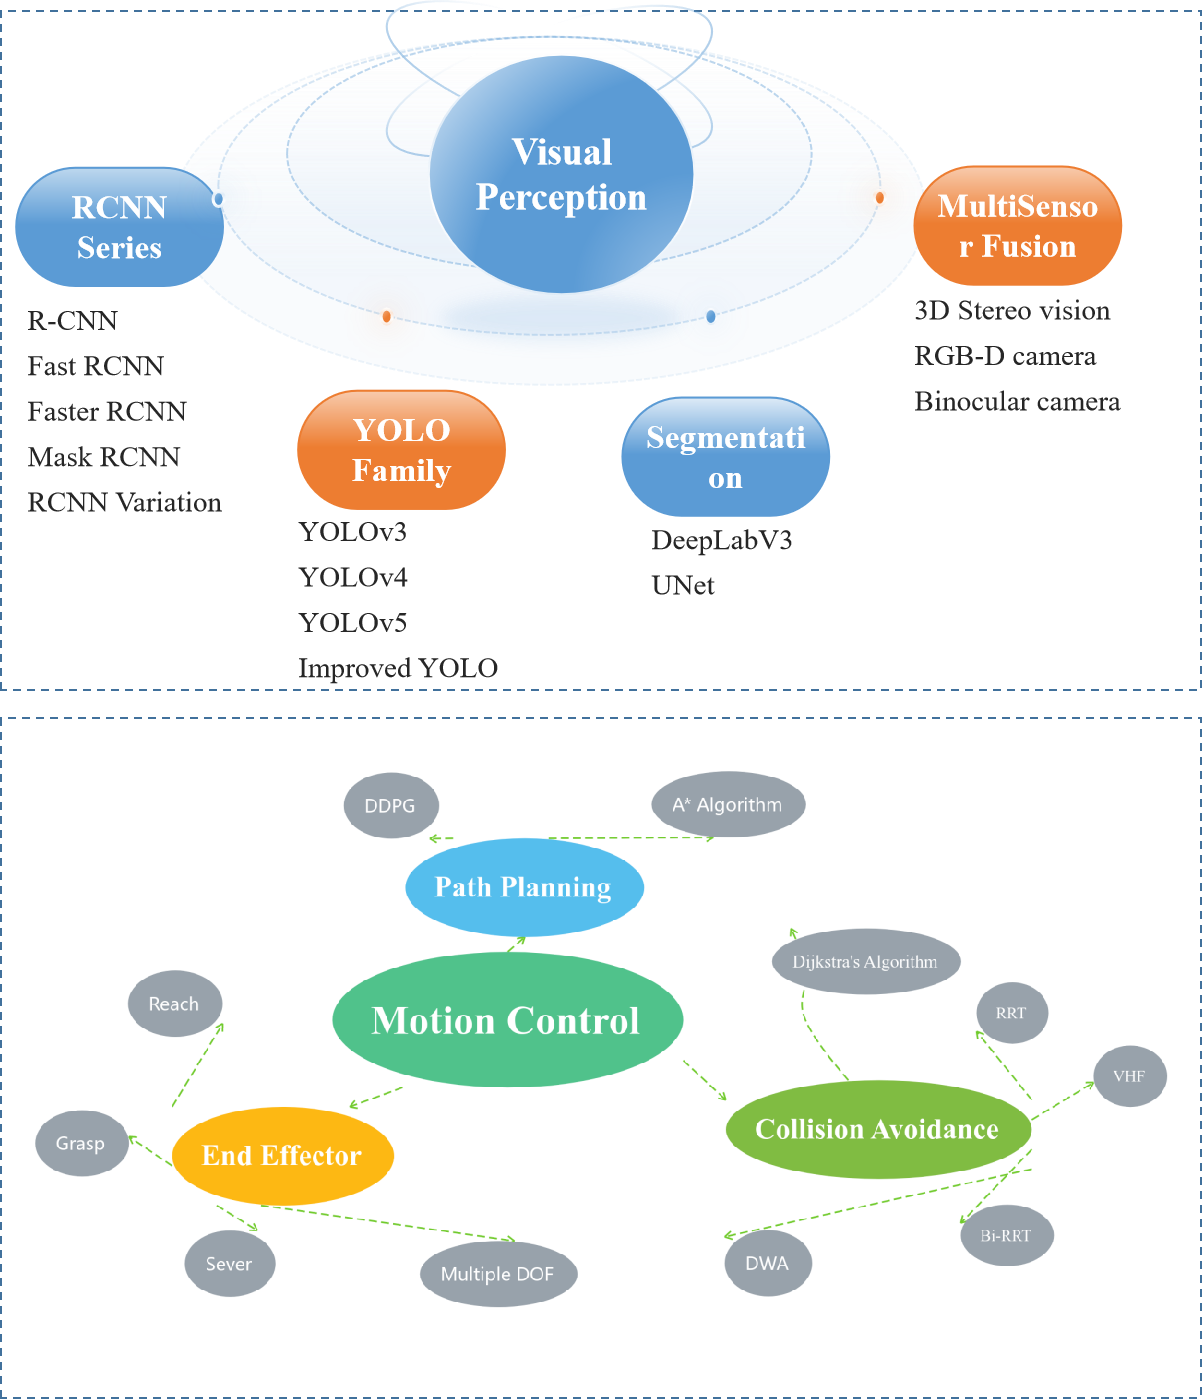
\includegraphics[width=0.5\textwidth]{fig_struct4.png}
    \caption{The perception-action framework of autonomous Fruit-Picking robots.}
    \label{fig:struct}
\end{figure}

\begin{table*}[ht]
\scriptsize
\centering
\caption{Summary of Survey Papers on Smart Farming Technologies.} 
\label{tab:survey_summary}
\begin{tabular} {p{0.4cm}p{0.5cm}p{3cm}p{3.2cm}p{3cm}p{4.5cm}}
\toprule
\textbf{Ref.} & \textbf{Year} & \textbf{Focus of the Paper} & \textbf{Key Technologies} & \textbf{Challenges Addressed} & \textbf{Key Insights} \\ \midrule

\cite{mohamed2021smart} & 2021 & IoT applications in precision agriculture & IoT, AI, and RS & Data management, Scalability & IoT integration enhances real-time data usage for improved agricultural decision-making. \\ \midrule
\cite{friha2021internet} & 2021 & IoT for smart agriculture & IoT, emerging technologies & Integration and scalability & Comprehensive survey of IoT technologies and their applications in smart agriculture \\ \midrule
\cite{martos2021ensuring} & 2021 & RS in Agriculture 5.0 & RS, AI, Big Data & Data processing complexity, high costs & Integration with AI and big data can enhance agricultural sustainability \\ \midrule
\cite{li2023mta} & 2023 & MTA - YOLACT for cherry tomato robotic harvesting & MTA - YOLACT, instance segmentation & Accurate identification of fruit bunch, pedicel and main stem & Enables precise visual support for cherry tomato harvesting robot's end - effector motion planning \\ \midrule
\cite{lytridis2021overview} & 2021 & Cooperative robotics in agriculture & Cooperative robotics & Coordination and efficiency & Reviews the use of cooperative robotics in agriculture, highlighting coordination and operational efficiency \\ \midrule
\cite{li2023multi}  & 2023 & Multi-arm coordination for efficient apple harvesting & Collaborative control, priority-based task scheduling & Low single-arm efficiency, collision risks & Framework enhancing throughput via coordinated motion \\ \midrule
\cite{hou2023overview} & 2023 & Machine vision in recognition and localization of fruit and vegetable harvesting robots & Machine vision sensors (monocular, stereo, etc.), vision algorithms & Complex background, illumination, fruit overlap and occlusion & Outlines application, challenges and future directions of machine vision in this field \\ \midrule
\cite{suresh2023selective} & 2023 & Evolution of selective fruit detection \& localization & Traditional vs. DL vision methods & Variability in fruit types, environmental interference & Comparative framework for robust visual system design \\ \midrule
\cite{gai2022fruit} & 2022 & Fruit and vegetable picking robot movement planning & Path planning algorithms (global and local) & Efficient and safe movement path planning in complex orchard environments & Summarizes motion planning algorithms and research results for fruit and vegetable picking robots \\ \midrule
\cite{liu2024hierarchical} & 2024 & Quadruped-robot integrated fruit harvesting & LiDAR-vision fusion, hierarchical trajectory planning & Unstructured terrain mobility, precise manipulation & Integration of legged mobility with picking operations \\ \midrule
\cite{darwin2021recognition} & 2021 & Recognition of bloom/ yield in crops using DL & DL, crop yield estimation & Accurate yield estimation & Reviews DL models for bloom and yield recognition in smart agriculture \\ \midrule
\cite{navas2021soft} & 2021 & Soft grippers for crop harvesting & Robotics, soft grippers & Delicate handling of crops & Reviews the development and application of soft grippers in automated crop harvesting \\ \midrule
\cite{wang2023biologically} & 2023 & Biologically inspired robotic perception - action for soft fruit harvesting & Conditional GAN, stereo vision, brain - inspired motion control & Labor shortage and difficult picking in vertical growing environments & Proposes bionic solution for strawberry harvesting, avoiding tedious data collection and annotation \\ \midrule
\cite{zhang2024automatic} & 2024 & Review of automatic fruit picking technology & Vision, Robotics, DL, Sensor fusion & Unstructured environments, Occlusion, Real-time, Multi-fruit & Overviews latest advances, compares key methods, and highlights integration challenges and future trends. \\   \midrule
\cite{zhou2022intelligent} & 2022 & Intelligent robots for fruit harvesting & Robotics, AI & Automation challenges & Reviews recent advancements and future challenges in the development of intelligent fruit-harvesting robots \\ \midrule
\cite{xiong2021improved} & 2021 & Obstacle separation for fruit picking in clusters & DL, hybrid visual control loop & Obstacle interference in clustered fruit picking & Improves obstacle separation accuracy and fruit picking success rate in complex environments \\ \midrule
\cite{rajendran2024towards} & 2023 & Autonomous selective harvesting: perception, design, motion planning & Robot perception, design, motion planning & Challenges in perception, design, motion planning and control for selective harvesting & Guides the development of more autonomous and efficient harvesting robots via multi - aspect analysis \\ \midrule
\cite{mingyou2024orchard} & 2024 & Orchard - wide visual perception and autonomous operation of fruit picking robots & Local object perception, global mapping, autonomous operation planning & Limitations of vision algorithms, map construction interference, low module coordination & Systematically reviews key technologies and provides theoretical guidance for orchard - wide autonomous operation of picking robots \\ 
\bottomrule
\end{tabular}
\end{table*}
\iffalse
In contrast to existing reviews summarized in Table~\ref{tab:survey_summary}, which primarily focus on isolated aspects such as individual sensor applications, specific model architectures, or single motion planning algorithms, this survey offers an integrated perspective on the holistic development of autonomous fruit-picking robots. While prior works have advanced understanding of multi-sensor fusion, DL-based detection, and path planning techniques, they often lack systematic integration of these components, leaving gaps in addressing the end-to-end challenges of real-world harvesting. Specifically, existing reviews insufficiently explore how sensor fusion can be optimally paired with DL models to enhance detection robustness under variable conditions, and they rarely connect visual perception directly to motion planning strategies tailored for unstructured agricultural environments.

This survey aims to bridge these gaps by highlighting the synergistic application of sensor fusion with DL algorithms to mitigate real-world detection limitations, as well as focusing on robotic systems that integrate path planning and collision avoidance in complex environments, as illustrated in Figure \ref{fig:struct}. The main contributions are outlined as follows:
\begin{itemize}
\item A comprehensive comparative analysis of sensing technologies in fruit-picking robotics, with a focus on multi-modality data fusion strategies to enhance perception accuracy and operational efficiency in dynamic agricultural settings.
\item An in-depth examination of segmentation models, including R-CNN families and YOLO series, with emphasis on challenge-specific solutions such as precise pick-point detection, real-time performance optimization, maturity assessment, and contour-based classification.
\item A thorough evaluation of motion planning algorithms designed explicitly for unstructured agricultural environments, emphasizing their integration with perception systems to ensure reliable obstacle avoidance and efficient path generation.
\end{itemize}
\fi

Existing reviews summarized in Table~\ref{tab:survey_summary} have laid valuable groundwork in autonomous fruit-picking robotics, however, they predominantly focus on fragmented components: individual sensor deployments (e.g., IoT or remote sensing in isolation \cite{mohamed2021smart,martos2021ensuring}), standalone model advancements (e.g., MTA-YOLACT for segmentation \cite{li2023mta}), or single-algorithm path planning (e.g., hierarchical trajectory methods \cite{liu2024hierarchical}). 
%While these works have advanced understanding of multi-sensor fusion, DL-based detection, and motion control techniques, 
They lack a critical systems-level perspective—failing to address how these components interact as an integrated ecosystem.
Notably, prior reviews overlook three pivotal gaps: (1) they rarely explore how multi-sensor fusion (e.g., LiDAR-vision integration \cite{liu2024hierarchical}) can be strategically paired with DL models to enhance robustness against real-world variability like occlusion or lighting changes; (2) they insufficiently connect visual perception (e.g., ripeness detection \cite{hou2023overview}) to context-aware motion planning tailored for unstructured orchards; and (3) they neglect the end-to-end optimization of collaborative systems (e.g., multi-arm coordination \cite{li2023multi}) that bridge perception, planning, and actuation.

This survey addresses these limitations by adopting a holistic "perception-action" framework. It uniquely emphasizes the synergistic integration of: (1) multi-modality sensor fusion (combining IoT, remote sensing, and vision \cite{mohamed2021smart,martos2021ensuring,liu2024hierarchical}) with DL models (e.g., evolved YOLO architectures) to mitigate detection fragility in dynamic environments; (2) visual perception outputs (e.g., fruit stem localization \cite{li2023mta}) with adaptive path planning (e.g., LiDAR-fused trajectory optimization \cite{liu2024hierarchical}) for seamless operation in unstructured terrain; and (3) collaborative robotics principles \cite{lytridis2021overview,li2023multi} with system-level efficiency analysis to address scalability challenges.
The core contributions of this survey are thus:
\begin{itemize}
\item A systematic analysis of how multi-sensor fusion strategies can be optimally aligned with DL models to enhance detection robustness across diverse agricultural scenarios, filling the gap in fragmented sensor-model discussions.
\item An integrated exploration of perception-to-action pipelines, connecting visual insights %(e.g., defect detection \cite{hou2023overview})
 to motion planning algorithms
 % (e.g., Bi-RRT, DDPG \cite{gai2022fruit,rajendran2024towards}) 
 specifically tailored for orchard complexity.
\item A critical evaluation of collaborative robotic systems that unify multi-arm coordination %\cite{li2023multi} 
with cost-effective design principles 
%\cite{zhang2024automatic}
, addressing scalability barriers overlooked in prior component-focused reviews.
\end{itemize}

The main technology structure in this paper is organized as follows illustrated in Figure \ref{fig:struct}. Section II describes the overall methodology, including the search strategy, paper selection, and synthesis of findings. Section III provides a synthesis and comparative discussion of data acquisition approaches through multi-sensor fusion.
%analysis of existing fruit-picking methodologies, focusing on emerging challenges, the evolution of AI vision methods, and strategies to overcome limitations in detection and motion planning. 
Section IV discusses advances in visual perception for fruit-picking robotics, covering state-of-the-art vision models (including R-CNN, YOLO, and segmentation), and challenge-oriented solutions. Section V reviews advances and trends in motion control for robotic fruit harvesting, emphasizing algorithmic path planning, obstacle avoidance, and developments in motion planning and control. Section VI presents recent progress and future directions in autonomous fruit harvesting technologies. Finally, Section VII concludes the paper, summarizing key findings and outlining prospects for future research.



\section{Survey Methodology}
This survey adheres to the PRISMA guidelines to ensure a transparent and thorough literature review. The primary objective is to identify and analyze highly cited papers that have significantly contributed to the field of fruit-picking robotics, the outline of which is shown in Figure~\ref{fig:prisma1}.
% The methodology consists of several stages: defining search criteria, selecting relevant papers, extracting data, and synthesizing the findings.
To enhance the clarity, coherence, and conciseness of the survey, the AI language model ChatGPT, developed by OpenAI, was employed. ChatGPT assisted in rephrasing text, ensuring each paragraph flowed seamlessly into the next and the overall narrative maintained a professional tone. The model was also used to generate summaries of individual papers, which were then reviewed and refined to match the context and requirements of this survey. The integration of ChatGPT into the writing process helped streamline the content organization and improve the paper's readability. The utilization of ChatGPT in academic writing has been discussed in detail by Gruda and Dritjon~\cite{gruda2024three}.
\begin{figure}[h!]
    \centering
    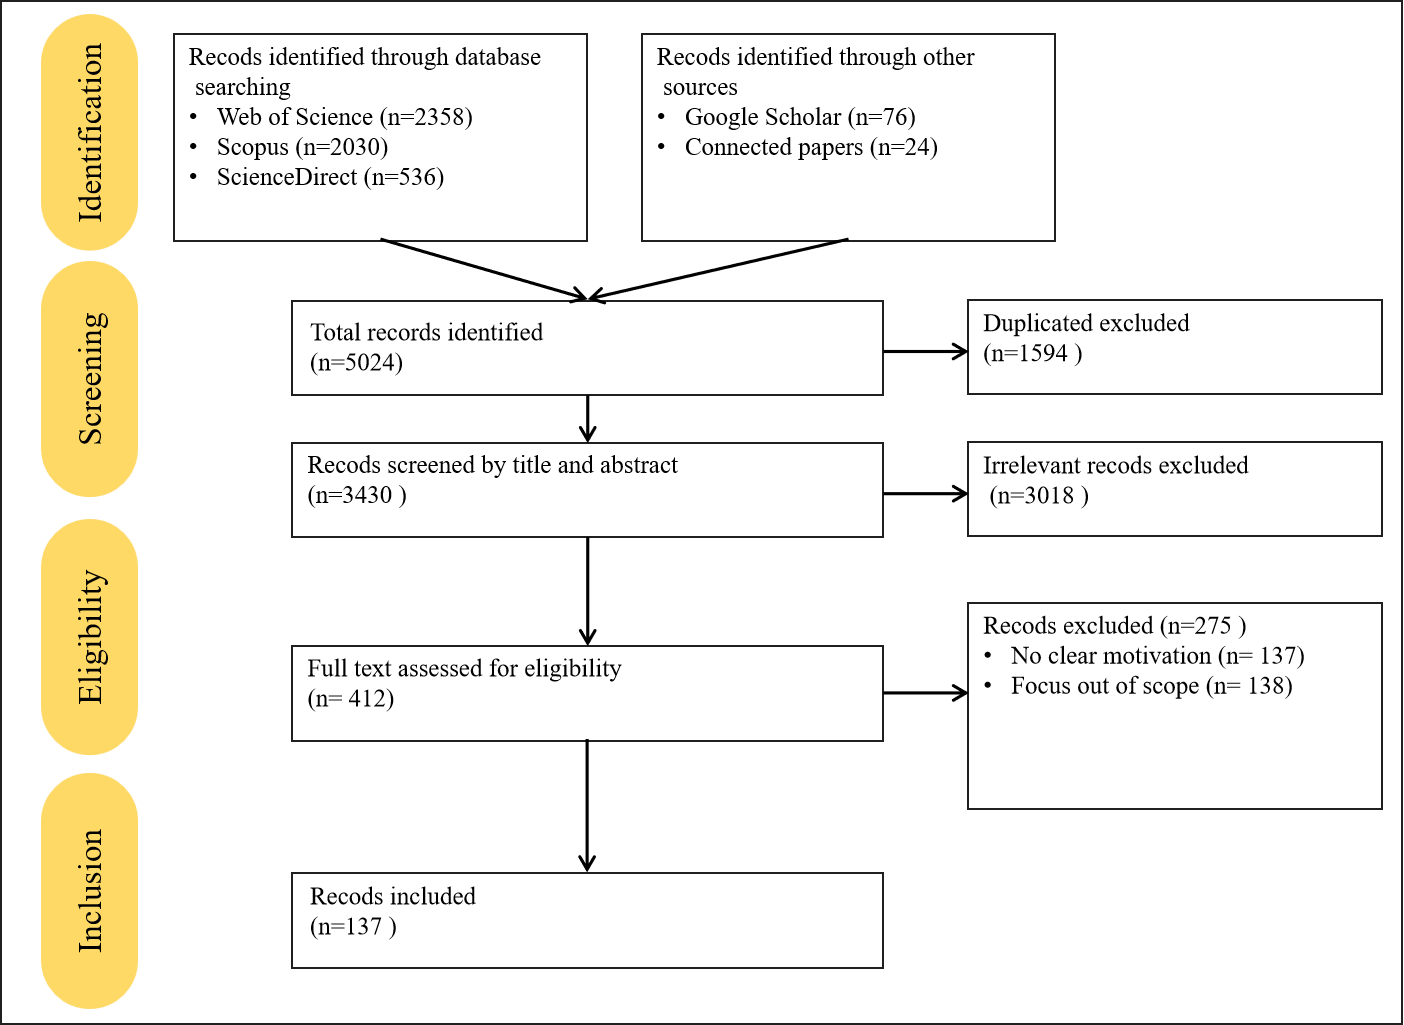
\includegraphics[width=0.5\textwidth]{fig_prisma1.png}
    \caption{Flow diagram depicting the identification and selection of publications to be included in this review.}
    \label{fig:prisma1}
\end{figure}

We began our research by systematically searching three well-established scientific databases, Web of Science (WoS), ScienceDirect and Scopus, to assemble a comprehensive collection of publications related to autonomous fruit-picking robots. The keywords used for these searches are listed in Table~\ref{tab:keywords}. The search was limited to English-language articles published between 2015 and 2024. This process resulted in 2358 records from WoS, 536 from ScienceDirect and 2030 from Scopus, as well in 100 from Google Scholar and Connected Papers, for a combined total of 4924 records prior to screening. To further ensure the completeness of our dataset, we also performed supplementary searches via Google Scholar and the Connected Papers , yielding an additional 76 and 24 records, respectively. In total, 5024 publications were identified in this initial phase.

Of the 5024 records initially identified, a comprehensive screening process was conducted to ensure the quality and relevance of the included studies. First, duplicates were identified and removed, resulting in 3430 unique entries. Manual screening was then performed without the aid of automation tools. During the title screening phase, 3018 records were excluded based on apparent irrelevance to the review topic. The remaining studies underwent abstract screening, which further reduced the collection to 412 potentially relevant records. Finally, full-text reviews were conducted on these entries to assess their fit with the review criteria.

\begin{table}[ht]
\scriptsize
\caption{Keywords and Criteria Used in Preliminary Database Search.} 
\label{tab:keywords} 
\begin{tabular}{p{0.3\linewidth} p{0.5\linewidth}}
\hline
\textbf{Criteria} & \textbf{Terms} \\ \hline
\textbf{Database}  &  Web of Science, Scopus, ScienceDirect \\
\textbf{Search Field} & Title, Keywords and Abstract\\
 & fruit-picking robot (Title) or fruit-picking robot (Abstract) or fruit-picking robot (Keyword Plus) or harvesting robot (Title) or harvesting robot (Abstract) or harvesting robot (Keyword Plus) or harvesting robotics (Title) or harvesting robotics (Abstract) or harvesting robotics (Keyword Plus)\\
\textbf{Language} & English \\
\textbf{Publication Date} & From 2015 TO 2024 \\ \hline 
\end{tabular}
\end{table}

The inclusion criteria for this review were as follows: (i) records describing fruit picking methods involving visual detection and segmentation; (ii) records focused on robot motion control applications such as path planning and collision avoidance; (iii) explicit statements regarding the motivation behind agricultural robot harvest; (iv) Records focused on the development, application, and evaluation of harvesting robots; (v) publications in the form of journal articles or conference proceedings; and (vi) empirical research based on experimental results rather than purely simulation-based studies.

Papers were excluded if they: (i) did not meet the above inclusion criteria; (ii) were review articles, surveys, or book chapters; (iii) lacked a clearly articulated motivation for agriculture robot; (iv) relied solely on simulation without experimental validation; or (v) were unavailable or inaccessible in full text.

\iffalse
\subsection{Search Strategy and Selection Criteria}
The search criteria were designed to capture a broad range of research papers related to fruit-picking robotics. Databases such as Web of Science (WoS), Scopus, and ScienceDirect were utilized for a comprehensive search. 
We restricted our search to titles and abstracts to ensure relevance, using the following keywords:
\begin{itemize}
    \item harvest(ing) robot(s)
    \item harvest robotics
    \item fruit-picking robot
    \item agricultural robot
%    \item"crop harvesting automation"
\end{itemize}

Inclusion criteria were set to include:
%\begin{enumerate}
\begin{itemize}
    \item Studies published between 2015 and 2024.
    \item Peer-reviewed journal articles and conference papers.
    \item Studies focusing on the development, application, and evaluation of harvesting robots.
    \item Studies addressing vision-based detection, learning-based approaches, and arm motion planning in harvesting robots.
\end{itemize}

Exclusion criteria were:
%\begin{enumerate}
\begin{itemize}
    \item Studies not written in English.
    \item Studies unrelated to agricultural robots.
    \item Review articles and editorials to focus on original research.
\end{itemize}

\subsection{Paper Selection}
The selection process involved screening the titles and abstracts of the papers to identify those that met the inclusion criteria. Full-text reviews were then conducted to ensure relevance and quality. Papers with many citations were prioritized, as they will likely have made substantial contributions to the field.
Data extraction focused on capturing key information from each paper, such as the research problem, proposed solution, methodology, and results. This information was organized into a structured format to facilitate comparison and analysis.
The findings from the selected papers were synthesized to provide a comprehensive overview of the current research in fruit-picking robotics. This synthesis aimed to identify common themes, challenges, and gaps in the literature and highlight promising directions for future research.
The initial search yielded 5024 studies. After removing duplicates, 3430 studies remained. Titles and abstracts were screened for relevance, resulting in 412 studies for full-text review. After a detailed assessment, over 130 studies met the inclusion criteria and were included in the systematic review.
Data were extracted using a standardized form, capturing:
\begin{itemize}
    \item Author(s) and year of publication
    \item Study objectives
    \item Methodological approach
    \item Key findings
    \item Challenges addressed
    \item Performance metrics and evaluation
\end{itemize}

\subsection{Synthesis of Findings}
The findings from the selected papers were synthesized to provide a comprehensive overview of the current research in fruit-picking robotics. This synthesis aimed to identify common themes, challenges, and gaps in the literature and highlight promising directions for future research.
Results were synthesized to summarize the main themes identified: vision-based detection, learning-based approaches, and arm motion planning in harvesting robots. This synthesis offered a comprehensive overview of current research trends, gaps, and advancements in the field.
%\subsection{Summary}
Following the PRISMA guidelines, this systematic review provides a comprehensive and transparent overview of the research on harvesting robots published between 2015 and 2024, yielding the following Figure \ref{fig:prisma}.

\begin{figure}[h!]
    \centering
    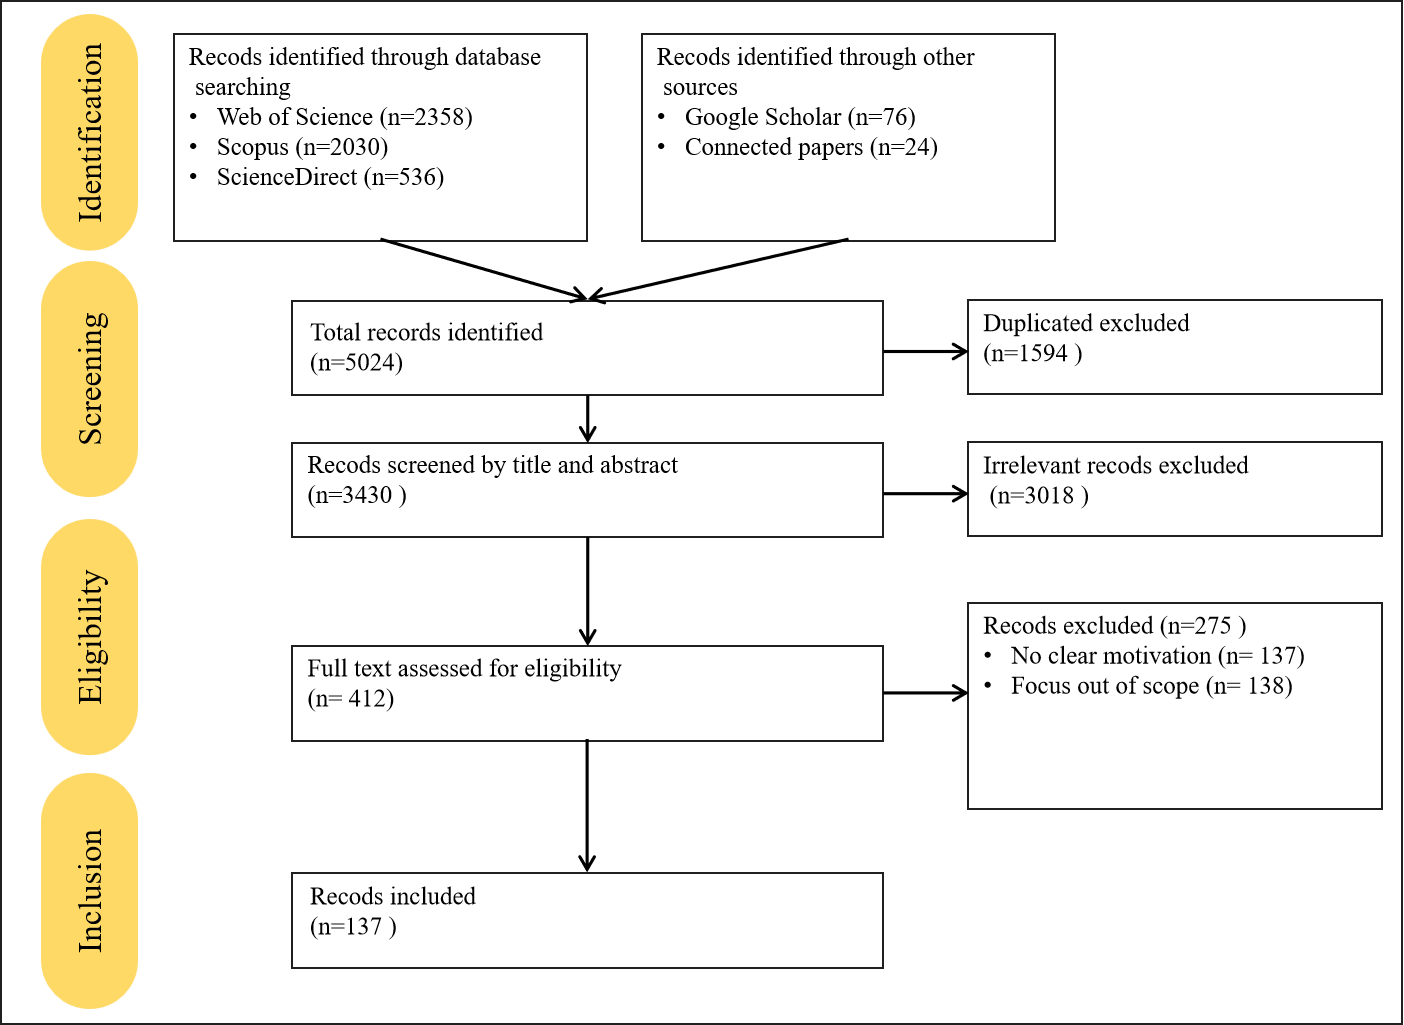
\includegraphics[width=0.5\textwidth]{fig_prisma1.png}
    \caption{Flow diagram depicting the identification and selection of publications to be included in this review.}
    \label{fig:struct}
\end{figure}

By incorporating ChatGPT, the methodological rigor of this survey was enhanced, ensuring a comprehensive and coherent review of the state-of-the-art in autonomous fruit-picking robotics.
\fi
\iffalse
\section{Synthesis and Comparative Analysis of Fruit-Picking Methodologies}
The review papers discussed in this section underscore the profound significance of the challenges, trends, limitations, and advancements in fruit-picking robotics. Analyzing these review papers aims to identify key insights and gaps in the existing research, facilitating a comprehensive understanding of state-of-the-art technologies and their practical applications.

\subsection{Emerging Challenges and Future Directions in Autonomous Fruit Harvesting}

Despite significant advancements in the field, fruit-picking robots still face numerous practical challenges that limit their widespread adoption. These include accurately detecting fruit under occlusion and dense foliage, making the system scalable across diverse environments, balancing detection efficiency with accuracy, and maintaining robustness under varying field conditions. The following discussion reviews key issues identified in recent literature and summarises state-of-the-art strategies for addressing these issues.

A persistent challenge, as highlighted in numerous reviews, is the issue of occlusion, whereby fruits are partially or fully obscured by leaves, branches or other fruits, which makes them difficult to detect accurately~\cite{lu2020survey, yu2020real}. This issue is exacerbated by variations in fruit appearance due to different growth stages and changing environmental conditions. Advanced solutions to this issue often involve ML models that use multi-modal data, such as RGB-D and thermal images, to improve detection reliability in occluded settings. Studies by Jia et al.~\cite{jia2020detection} and Gao et al.~\cite{gao2020multi}demonstrate how incorporating depth information can notably enhance detection performance in the presence of occlusion.
Closely related is the obstacle posed by dense foliage, which not only hides fruits but can also introduce false positives, making it difficult for algorithms to distinguish fruits from surrounding leaves~\cite{wan2020faster, fu2020faster}. To address this, researchers have explored the use of advanced segmentation models and depth information. In particular, Kang et al.~\cite{kang2020fruit, kang2020real} illustrated how instance and semantic segmentation can significantly bolster real-time fruit detection and harvesting performance amidst dense foliage. Comparative analyses indicate that, while both occlusion and dense foliage require sophisticated detection algorithms, integrating depth cues and enhanced segmentation techniques substantially improves performance.
Another critical challenge is ensuring the scalability of detection systems, i.e. maintaining their efficacy across varied environments, fruit types, and operational scales~\cite{yu2019fruit, tu2020passion}. This is particularly important for commercial applications, since robots must function reliably in diverse orchard conditions. Transfer learning and robust model development have been proposed as potential solutions, enabling adaptation to new tasks with minimal retraining. The effectiveness of these approaches in generalising detection models has been demonstrated by Liu et al.~\cite{liu2016method} and Xu et al.~\cite{xu2019real}.
Efficiency in term of both in detection speed and resource utilisation is also a central concern for the practical deployment of robotic harvesters~\cite{ge2019fruit, lin2020color}. Algorithms such as YOLO are notable for their real-time detection capabilities~\cite{liu2020yolo, lawal2021tomato}, whereas models from the R-CNN series generally offer greater accuracy but require more computational resources~\cite{fu2018kiwifruit, chu2021deep}. This highlights the ongoing need to balance speed and accuracy, optimising both for practical, large-scale agricultural use.

Finally, developing detection systems that can withstand natural environmental variability, such as fluctuating light, weather, and terrain, remains an important hurdle. Rahnemoonfar et al.~\cite{rahnemoonfar2017deep} and Luo et al.~\cite{luo2018vision} emphasised the need for advanced vision technologies capable of maintaining high accuracy under such variable conditions. In this regard, stereo vision systems as demonstrated by Luo et al.~\cite{luo2016vision} and Kang et al.~\cite{kang2020real} have been explored to improve detection robustness in the field.

\subsection{Evolution of AI Vision Methods for Fruit Detection and Localization}

Over the past decade, there have been rapid and transformative developments in fruit detection technologies for agricultural robotics. This section reviews milestone advancements, tracing the transition from traditional vision methods to DL and the integration of multimodal sensors. It also covers emerging trends, such as synthetic data and IoT-enabled solutions.

While early fruit detection systems primarily employed classical computer vision techniques; however, a significant shift has occurred towards DL-based approaches, particularly convolutional neural networks(CNNs) and their derivatives. These have demonstrated clear advantages in handling complex detection tasks ~\cite{Ting:2024_ieee,Goay:2021_access,sa2016deepfruits}. This transition is well documented in several reviews, which highlight that DL is more accurate and adaptable than earlier methods.
Alongside advances in model architecture, integrating multiple sensor modalities — most notably combining RGB and depth data — has become a key trend, greatly enhancing robustness in challenging conditions such as variable lighting and occlusion~\cite{jun2021towards}. Such sensor fusion, complemented by hardware innovations such as advanced end-effectors, improves not only detection accuracy but also the overall harvesting efficiency  while reducing  fruit damage.
The proliferation and utilisation of large-scale annotated datasets represent is another cornerstone in the evolution of detection technologies. Comprehensive datasets have enabled more effective training, benchmarking, and model comparison, thereby accelerating research progress and ensuring more reliable evaluations ~\cite{yu2020real,yu2019fruit,wan2020faster}. Additionally, the increasing use of synthetic datasets provides a valuable solution to the issue of limited data, expanding the range and quantity of training samples to enhance model robustness and generalisation~\cite{barth2018data}.
Despite these advancements, no single technology has emerged as a panacea. Review papers emphasise the necessity of combining advanced detection models, sensor fusion and efficient algorithmic frameworks to address the varied challenges of field environments effectively. Improving model generalisability, real-time performance and multimodal integration remain key priorities for future research.
Finally, integrating IoT technologies with image recognition, as demonstrated by Horng et al.~\cite{horng2019smart}, is set to further enhance the capabilities of fruit-picking robots. These developments point towards a future where real-time monitoring, automated decision-making, and intelligent control will significantly increase agricultural efficiency and productivity.

\subsection{Overcoming Limitations in Detection and Motion Planning for Fruit-Picking Robots}
While these papers provide valuable contributions to the field, several limitations must be addressed, particularly in fruit-picking robots' detection and motion planning.
Many surveys, such as~\cite{lu2020survey}, emphasize the importance of robust detection algorithms for precision agriculture. However, a notable lack of standardized datasets and benchmarking protocols makes it challenging to effectively compare the performance of different detection techniques.
Papers like~\cite{mohamed2021smart} and~\cite{darwin2021recognition} discuss the integration of AI and DL for crop detection. Despite the advancements, these surveys often overlook the challenges of achieving real-time detection and maintaining robustness under varying environmental conditions, such as changes in lighting and occlusions caused by dense foliage.
Surveys on robotic applications, such as~\cite{ampatzidis2017ipathology} and~\cite{zhou2022intelligent}, highlight significant progress in motion planning algorithms. However, their adaptation to real-world agricultural environments remains underexplored, particularly in navigating complex and dynamic field conditions while avoiding obstacles. 
While technological advancements in motion planning, discussed in papers like~\cite{jia2020apple} and~\cite{zhang2020technology}, show promise, there is insufficient focus on scalability and operational efficiency, especially when transitioning from controlled environments to large-scale agricultural fields.
 
In contrast, our survey paper aims to address these limitations by focusing on detection and motion planning for fruit-picking robots. We propose a framework for creating and using standardized datasets, ensuring compatibility, and facilitating benchmarking of various detection techniques. 
Our review includes advanced detection algorithms designed to achieve real-time performance and maintain robustness across different environmental conditions, addressing challenges like occlusions and variable lighting.
We provide a thorough analysis of motion planning algorithms specifically designed to navigate agricultural fields' complex and dynamic conditions, ensuring reliable obstacle avoidance and efficient path planning.
Our survey emphasizes the importance of scalability and operational efficiency, offering insights into how advanced motion planning techniques can be effectively scaled for use in large agricultural fields. Thus, it bridges the gap between controlled environments and real-world applications.
By addressing these critical limitations, our survey paper builds upon the existing body of knowledge. It paves the way for future research and practical applications in the detection and motion planning aspects of innovative farming technologies.


\begin{figure}[h]
    \centering
    \begin{subfigure}[t]{0.45\textwidth}
        \centering
        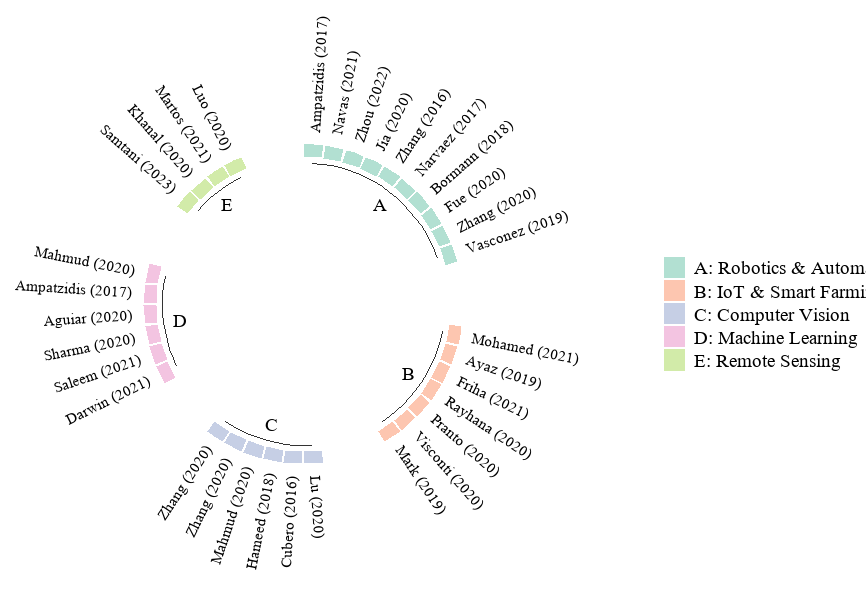
\includegraphics[width=\textwidth]{fig_review_tech.png}
        \caption{Distribution of Review papers by Main Technology Discussed }
        \label{fig:tech1}
    \end{subfigure}
    \hspace{0.05\textwidth}
    \begin{subfigure}[t]{0.4\textwidth}
        \centering
        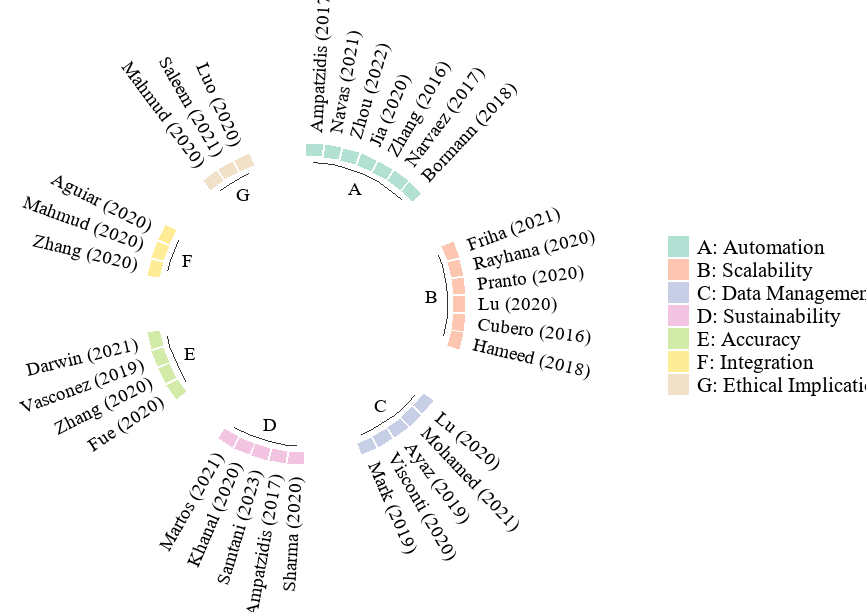
\includegraphics[width=\textwidth]{fig_review_challenge.png}
        \caption{Distribution of Review papers by Main Challenges Discussed}
        \label{fig:challenge1}
    \end{subfigure}
    
    \caption{Figures illustrating the Distribution of Review papers Discussed.}
    \label{fig:combined_review_figures}
\end{figure}

Figure \ref{fig:combined_review_figures} provides a comprehensive visualization of the distribution of review papers on fruit-picking robotics in past decade. The radar charts in Figures \ref{fig:tech1} and \ref{fig:challenge1} offer insights into the primary focus areas and challenges highlighted in the literature. Specifically, Figure \ref{fig:tech1} shows that the predominant technologies discussed include Robotics \& Automation, IoT \& Smart Farming, and Computer Vision, with fewer papers addressing ML and RS. Figure \ref{fig:challenge1} reveals that the main challenges tackled by these studies are automation, scalability, and data management, with ethical implications, integration, and sustainability being less frequently addressed. 
This comprehensive analysis underscores the critical role of advanced technologies in enhancing fruit-picking robots' efficiency and effectiveness while highlighting ongoing challenges and areas for future research.

%\onecolumn
%\begin{scriptsize}
%\begin{table*}{p{0.4cm}p{0.5cm}p{3cm}p{3.2cm}p{3cm}p{5cm}}
%\begin{longtable}{p{0.4cm}p{0.5cm}p{3cm}p{3.2cm}p{3cm}p{5cm}}

\begin{table*}[ht]
\scriptsize
\centering
\caption{Summary of Survey Papers on Smart Farming Technologies (part 1)} 
\label{tab:survey_summary}
\begin{tabular} {p{0.4cm}p{0.5cm}p{3cm}p{3.2cm}p{3cm}p{5cm}}
\toprule
\textbf{Ref.} & \textbf{Year} & \textbf{Focus of the Paper} & \textbf{Key Technologies} & \textbf{Challenges Addressed} & \textbf{Key Insights} \\

\cite{lu2020survey} & 2020 & Public datasets for computer vision in precision agriculture & Computer vision, datasets & Lack of standardized datasets & Identifies and reviews available datasets, highlighting gaps and opportunities for dataset standardization \\ \midrule
\cite{mohamed2021smart} & 2021 & IoT applications in precision agriculture & IoT, AI, and RS & Data management, Scalability & IoT integration enhances real-time data usage for improved agricultural decision-making. \\
\midrule
\cite{ampatzidis2017ipathology} & 2017 & Robotic applications in plant pathology and management. & Machine vision, AI, ML, and intelligent technologies for precision agriculture. & Diagnostic specificity in disease management, adaptation of technologies in uncontrolled environments. & Highlights the potential of advanced technologies to improve the accuracy and efficiency of disease diagnostics in agriculture, stressing the need for more robust systems. \\ \midrule
\cite{samtani2019status} & 2023 & Review of the strawberry industry in the U.S., including production practices and market trends. & None specific; broad industry overview. & Regional production challenges, labor shortages, and market demand changes. & Highlights the adoption of protected culture to extend seasons, address market demands, and the need for regional research to overcome growing challenges. \\ \midrule
\cite{navas2021soft} & 2021 & Soft grippers for crop harvesting & Robotics, soft grippers & Delicate handling of crops & Reviews the development and application of soft grippers in automated crop harvesting \\ \midrule
\cite{zhou2022intelligent} & 2022 & Intelligent robots for fruit harvesting & Robotics, AI & Automation challenges & Reviews recent advancements and future challenges in the development of intelligent fruit-harvesting robots \\ \midrule
\cite{darwin2021recognition} & 2021 & Recognition of bloom/ yield in crops using DL & DL, crop yield estimation & Accurate yield estimation & Reviews DL models for bloom and yield recognition in smart agriculture \\ \midrule
\cite{jia2020apple} & 2020 & Apple harvesting robots & Robotics, automation & Efficient apple harvesting & Reviews the current state of apple harvesting robots, focusing on technological and operational challenges \\ \midrule
\cite{zhang2020technology} & 2020 & Mechanical harvest of fresh market apples & Mechanical harvesting, robotics & Efficiency and damage reduction & Discusses technological progress in mechanical harvesting, focusing on efficiency and reducing crop damage \\ \midrule
\cite{aravind2017task} & 2017 & Task-based agricultural robots & Mobile robotics, task automation & Task efficiency & Reviews task-based robotic systems for arable farming, focusing on efficiency and operational challenges \\ \midrule
\cite{lytridis2021overview} & 2021 & Cooperative robotics in agriculture & Cooperative robotics & Coordination and efficiency & Reviews the use of cooperative robotics in agriculture, highlighting coordination and operational efficiency \\ \midrule
\cite{aguiar2020localization} & 2020 & Localization and mapping in agriculture & Localization, mapping, robotics & Accurate localization & Surveys localization and mapping techniques for agricultural and forestry robots \\ \midrule
\cite{zhang2016development} & 2016 & Development of mechanical apple harvesting technology & Mechanical harvesting & Technological advancements & Reviews the development of mechanical harvesting technologies, focusing on progress and challenges \\ \midrule
\cite{bormann2018indoor} & 2018 & Indoor coverage path planning & Path planning, robotics & Coverage efficiency & Surveys indoor path planning techniques, focusing on implementation and analysis \\ \midrule
\cite{fue2020extensive} & 2020 & Mobile agricultural robots for cotton harvesting & Mobile robotics, cotton harvesting & Operational efficiency & Reviews mobile robots for cotton harvesting, focusing on operational efficiency and challenges \\ \midrule
\cite{ayaz2019internet} & 2019 & IoT-based smart agriculture & Wireless sensors, UAVs, cloud-based architectures & Data security, standardization, integration with traditional farming & Comprehensive review of IoT applications in agriculture, highlighting technological innovations and future trends \\ \midrule
\cite{saleem2021automation} & 2021 & Automation in agriculture using ML and DL & ML, DL & Automation and accuracy & Reviews recent developments in automation using ML and DL techniques in agriculture \\ \midrule
\cite{khanal2020remote} & 2020 & RS in agriculture & Satellite, UAS, manned aircraft, RS data types & Data accuracy, integration with existing practices, economic feasibility & Comprehensive review of RS applications, highlighting technological advancements and future trends \\ \midrule
\cite{friha2021internet} & 2021 & IoT for smart agriculture & IoT, emerging technologies & Integration and scalability & Comprehensive survey of IoT technologies and their applications in smart agriculture \\ \midrule
\cite{zhang2020state} & 2020 & Robotic grippers in agriculture & Robotics, grippers & Grasping efficiency & Reviews state-of-the-art robotic grippers, their applications, and control strategies in agriculture \\ \midrule
\cite{sharma2020machine} & 2020 & ML applications for precision agriculture & ML & Application diversity & Comprehensive review of ML applications in precision agriculture \\ \midrule
\cite{luo2020identifying} & 2020 & Spatiotemporal changes in crop harvesting areas & RS, GLASS LAI, phenology-based mapping & Lack of high-resolution, time-continuous crop data & High accuracy in crop classification, revealing significant changes in cropping patterns due to various factors \\ \midrule
\cite{cubero2016automated} & 2016 & Automated systems for citrus fruit inspection & Machine vision, automation & Inspection accuracy & Reviews machine vision-based automated systems for inspecting citrus fruits from field to postharvest \\ \midrule
%\cite{rayhana2020internet} &2020 & Review of IoT technologies in greenhouse farming & Identification of challenges in sensor technology and decision-making systems & IoT-enabled sensors and devices & N/A \\ \midrule
\cite{pranto2021blockchain} & 2020 & Blockchain and IoT in smart agriculture & Blockchain, smart contracts, IoT & Data security, transparency, trust in supply chains & Integration of blockchain enhances data security and efficiency, reducing the need for intermediaries \\ \midrule
\end{tabular}
\end{table*}

\begin{table*}[ht]
\scriptsize
\addtocounter{table}{-1}
\centering
\caption{Summary of Survey Papers on Smart Farming Technologies (part 2)} 
%\label{tab:survey_summary}
\begin{tabular} {p{0.4cm}p{0.5cm}p{3cm}p{3.2cm}p{3cm}p{5cm}}
\toprule
\textbf{Ref.} & \textbf{Year} & \textbf{Focus of the Paper} & \textbf{Key Technologies} & \textbf{Challenges Addressed} & \textbf{Key Insights} \\

\cite{narvaez2017survey} & 2017 & Ranging and imaging techniques for phenotyping & Ranging, imaging, phenotyping & Accuracy, and efficiency & Surveys techniques for precision agriculture phenotyping, focusing on ranging and imaging \\ \midrule
\cite{mahmud2020robotics} & 2020 & Robotics and automation in agriculture & Robotics, automation & Future applications & Reviews present and future applications of robotics and automation in agriculture \\ \midrule
\cite{vasconez2019human} & 2019 & Human-robot interaction in agriculture & Human-robot interaction & Interaction challenges & Surveys human-robot interaction in agriculture, highlighting current challenges \\ \midrule
\cite{hameed2018comprehensive} & 2018 & Fruit and vegetable classification techniques & Machine vision, classification & Classification accuracy & Comprehensive review of classification techniques for fruits and vegetables using machine vision \\ \midrule
\cite{liu2017research}& 2017 & Robotic harvesting in greenhouses & End-effectors, motion planning, control strategies & Precision and efficiency improvement & Comprehensive review of global research, identifies future research directions \\ \midrule
\cite{martos2021ensuring} & 2021 & RS in Agriculture 5.0 & RS, AI, Big Data & Data processing complexity, high costs & Integration with AI and big data can enhance agricultural sustainability \\ \midrule
\cite{visconti2020development} & 2020 & IoT-based farm management & IoT, WSN, BLE & Resource optimization, traceability & Integrated system for real-time monitoring and decision support \\ \midrule
\cite{mark2019ethics} & 2019 & Ethical analysis of AI and Big Data & AI, Big Data, SIS & Data ownership, privacy, digital divide & Ethical implications of SIS use, data privacy, economic impact \\ \midrule
%\cite{zhang2024automatic} & 2024 & Comprehensive review of automatic fruit picking technology & Vision-based detection, Robotic manipulation, DL, Sensor fusion, Multi-modal perception & Challenging unstructured environments, Fruit occlusion, Real-time operation, Multi-fruit adaptability & Summarizes state-of-the-art advances, compares core technical routes, highlights integration of perception and manipulation, and outlines future development trends and industry bottlenecks in automatic fruit picking. \\
\cite{zhang2024automatic} & 2024 & Review of automatic fruit picking technology & Vision, Robotics, DL, Sensor fusion & Unstructured environments, Occlusion, Real-time, Multi-fruit & Overviews latest advances, compares key methods, and highlights integration challenges and future trends. \\ 
%\cite{rajendran2024towards} & 2024 & Review of autonomous selective harvesting & Robot perception, Design, Motion planning, Control algorithms & Complex crop environments, Selectivity, System integration & Provides a unified perspective on perception-driven selective harvesting challenges and research priorities. \\
\bottomrule
%\endul{longtable}
\end{tabar}
\end{table*}

Table \ref{tab:survey_summary} provides a comprehensive summary of survey papers on innovative farming technologies, highlighting their key contributions, technologies discussed, challenges addressed, and key insights. The reviewed papers span various aspects of smart farming, including computer vision, IoT, AI, ML, and robotics. This table is a valuable resource for understanding the breadth of research in innovative farming technologies, identifying key trends, and pinpointing areas requiring further investigation and development.
\fi

\section{Data Acquisition Through Multi-Sensor Fusion}
Modern fruit-picking robotics increasingly relies on a diverse array of sensor technologies such as 3D stereo vision, RGB-D cameras, binocular vision, as well as integration with IoT, GIS, laser, and RS to obtain robust environmental and positional data. As summarized in %Table~\ref{table:comparison}, 
Figure~\ref{fig:camera}, these combined methodologies enable more exhaustive and accurate perception, greatly enhancing fruit detection and localization even in challenging agricultural conditions.
\begin{figure}[hbtp]
\centering
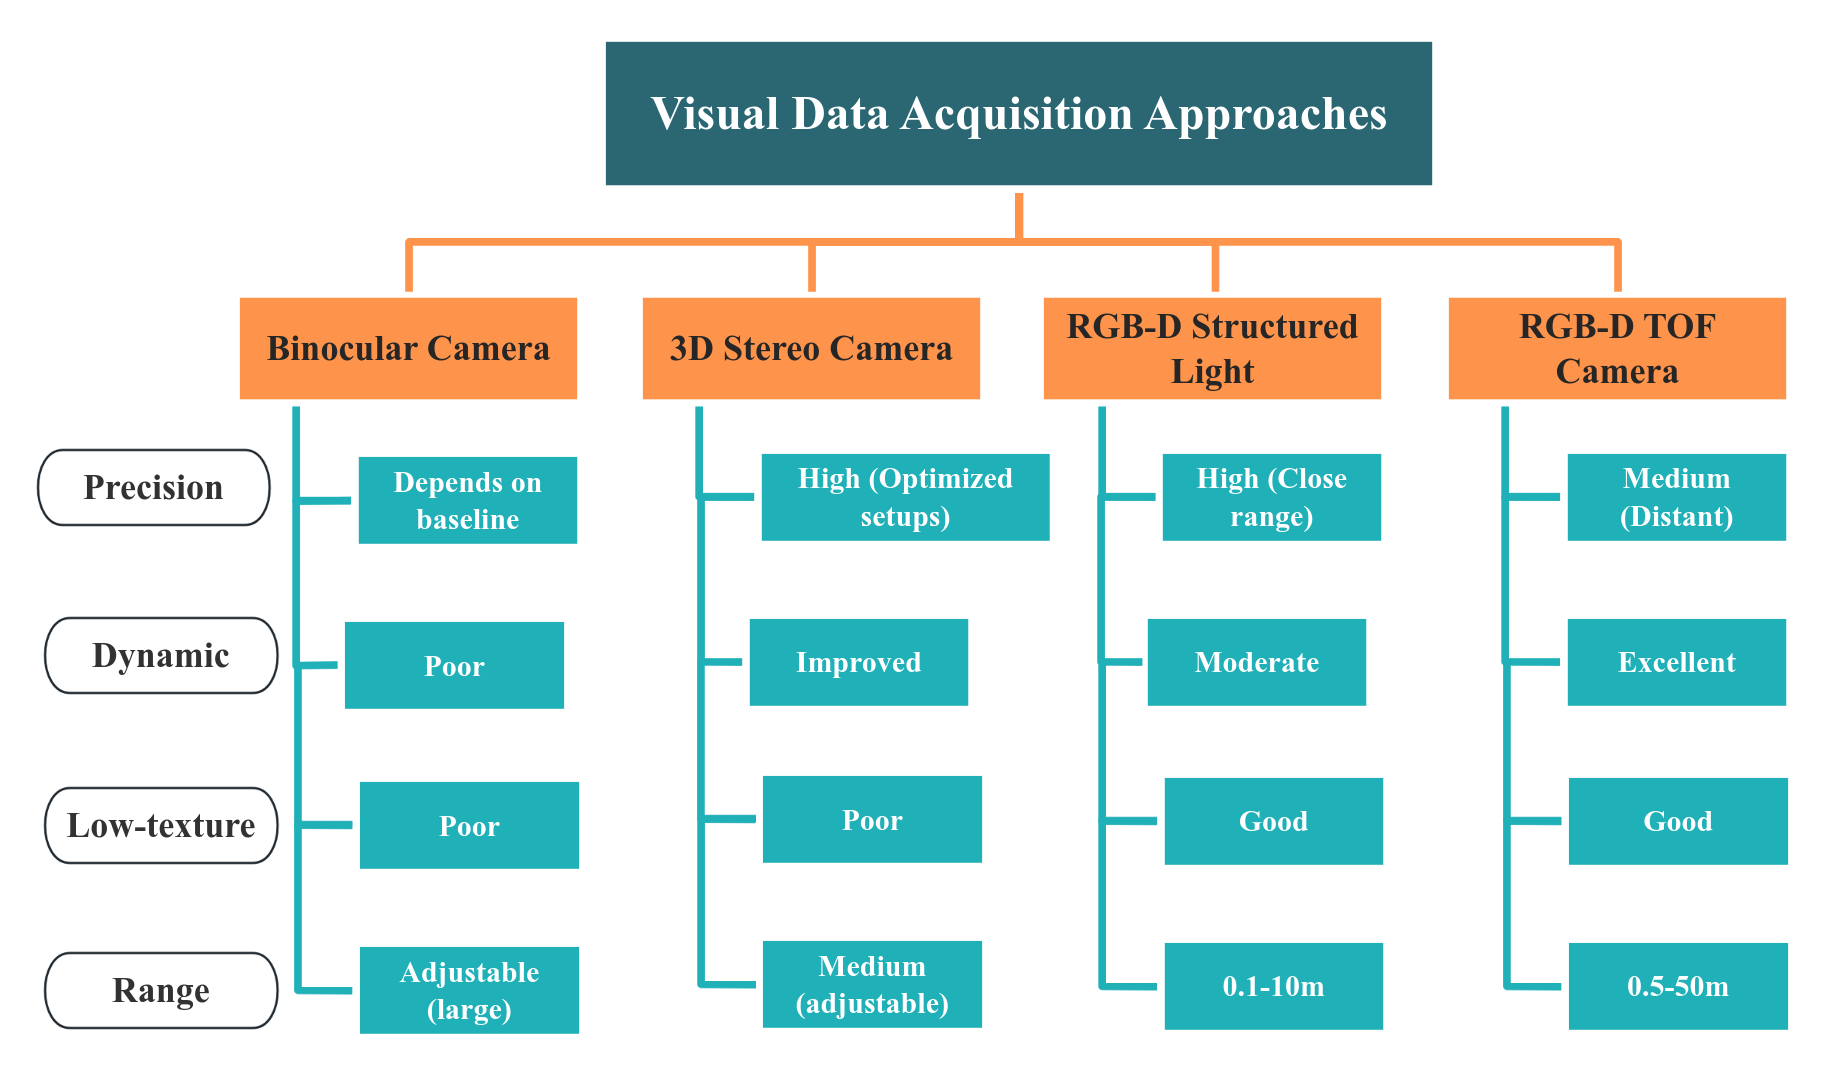
\includegraphics[width=0.52\textwidth]{fig_camera1.png}
\caption{The multi-modality data compare for object detection.}
\label{fig:camera}
\end{figure}
\begin{table*}[ht]
\scriptsize
\centering
\caption{Data Acquisition Approaches on Smart Farming Technologies.} 
\label{tab:dataset}
\begin{tabular} {p{0.4cm}p{0.5cm}p{3cm}p{3.2cm}p{3cm}p{5cm}}
\toprule
\textbf{Ref.} & \textbf{Year} & \textbf{Focus of the Paper} & \textbf{Key Technologies} & \textbf{Challenges Addressed} & \textbf{Key Insights} \\
\midrule
\cite{mohamed2021smart} & 2021 & IoT applications in precision agriculture & IoT, AI, and RS & Data management, Scalability & IoT integration enhances real-time data usage for improved agricultural decision-making. \\
\midrule
\cite{friha2021internet} & 2021 & IoT for smart agriculture & IoT, emerging technologies & Integration and scalability & Comprehensive survey of IoT technologies and their applications in smart agriculture \\ \midrule
\cite{martos2021ensuring} & 2021 & RS in Agriculture 5.0 & RS, AI, Big Data & Data processing complexity, high costs & Integration with AI and big data can enhance agricultural sustainability \\ \midrule
\cite{ayaz2019internet} & 2019 & IoT-based smart agriculture & Wireless sensors, UAVs, cloud-based architectures & Data security, standardization, integration with traditional farming & Comprehensive review of IoT applications in agriculture, highlighting technological innovations and future trends \\ \midrule
\cite{visconti2020development} & 2020 & IoT-based farm management & IoT, WSN, BLE & Resource optimization, traceability & Integrated system for real-time monitoring and decision support \\ \midrule
\cite{khanal2020remote} & 2020 & RS in agriculture & Satellite, UAS, manned aircraft, RS data types & Data accuracy, integration with existing practices, economic feasibility & Comprehensive review of RS applications, highlighting technological advancements and future trends \\ \midrule
\cite{pranto2021blockchain} & 2020 & Blockchain and IoT in smart agriculture & Blockchain, smart contracts, IoT & Data security, transparency, trust in supply chains & Integration of blockchain enhances data security and efficiency, reducing the need for intermediaries \\ \midrule
\cite{lu2020survey} & 2020 & Public datasets for computer vision in precision agriculture & Computer vision, datasets & Lack of standardized datasets & Identifies and reviews available datasets, highlighting gaps and opportunities for dataset standardization \\ \midrule

\cite{mark2019ethics} & 2019 & Ethical analysis of AI and Big Data & AI, Big Data, SIS & Data ownership, privacy, digital divide & Ethical implications of SIS use, data privacy, economic impact \\ \midrule
\cite{wang2016localisation} & 2016 & Binocular Stereo Vision, Wavelet Transform & High accuracy in unstructured settings & Recognition: 98.8\% unoccluded, 97.5\% occluded; Effective matching & Demonstrates robust litchi recognition and localization using stereo vision and advanced image processing in natural environments \\ \midrule
\cite{si2015location} & 2015 & Stereoscopic Vision, RRM & Accurate localization in unstructured environments & High recognition rate (over 89.5\%), minimal localization errors & Utilizes stereoscopic vision for precise 3D localization and effective apple recognition, enhancing robotic harvesting capabilities \\ \midrule	
\cite{luo2016vision} & 2016 & Binocular Stereo Vision & Precise cutting point localization & 87\% success rate, <0.7s processing time & Demonstrates the potential of stereo vision in robotic grape harvesting with high accuracy and efficiency \\ \midrule
\cite{barnea2016colour} & 2016 & RGB-D, Shape-Based 3D & Detection independent of color & Effective even in occluded conditions & Utilizes 3D shape and symmetry for robust detection, enhancing adaptability in agricultural robotics \\ \midrule	
\cite{li2020detection} & 2020 & DeepLabv3 + DBSCAN & Localization in natural environments & Detection accuracy 83.33\%, Execution speed 0.464s  & Utilizes RGB-D imaging and 3D clustering for precise localization and detection \\  \midrule
\cite{lin2019field} & 2019 & RGB-D, Bayes Classifier, Support Vector Machine (SVM) & Handling variable conditions and partial occlusions & F1 score of 0.9197; precise localization & Integrates RGB-D imaging with advanced ML techniques for robust fruit detection and localization \\ \midrule
\cite{gongal2018apple} & 2018 & 3D machine vision, TOF camera & Accurate size estimation in orchards & Accuracy: 69.1\% (3D coordinates), 84.8\% (pixel size)  & Combination of 3D coordinates and pixel size improves size estimation accuracy \\ \midrule
\cite{gene2019fruit}& 2019 & MTLS with LiDAR,3D point clouds from MTLS & Robust detection under varying conditions & Localization: 87.5\%, Identification: 82.4\%, F1-score: 0.858 & LiDAR-based system provides accurate 3D fruit localization unaffected by lighting variations \\ \midrule
\cite{sumesh2021integration}& 2024 & RGBVI, NDVI, CSM, OBIA & Accurate yield estimation & $R^2: 0.89$ & Integration of multiple data sources improves yield prediction accuracy \\ 
\bottomrule
%\endul{longtable}
\end{tabular}
\end{table*}

Among multi-sensor approaches, 3D stereo vision systems play a pivotal role by using dual cameras to estimate depth via triangulation, effectively mimicking human binocular vision. Early efforts include Wang et al.~\cite{wang2016localisation}, who developed a binocular stereo vision system for litchi localization, incorporating wavelet transforms and clustering methods to achieve high accuracy under natural lighting. Similarly, Si et al.~\cite{si2015location} advanced apple detection by enabling their stereo vision platform to recognize and localize multiple fruits simultaneously in variable environments. Luo et al.~\cite{luo2016vision} further demonstrated a grape-harvesting stereo system capable of quickly detecting cutting points and estimating yields with high efficiency.
RGB-D cameras which combine color information with depth sensing using time-of-flight or structured light have also proven highly beneficial. Barnea et al.~\cite{barnea2016colour} presented an RGB-D-based 3D detection method capable of analyzing both shape and symmetry, which is effective for sweet pepper harvesting even under complex conditions. Nguyen et al.~\cite{nguyen2016detection} showed that integrating depth with RGB data significantly improves apple detection and localization, especially under occlusion. Kusumam et al.~\cite{kusumam20173d} and Andújar et al.~\cite{andujar2016using} extended these principles to broccoli and cauliflower, using mobile RGB-D platforms to deliver precise 3D crop measurements crucial for automated harvest scheduling.
%The value of multi-perspective or adaptive camera positioning is highlighted by Hemming et al.\cite{hemming2014fruit}, whose sweet pepper studies revealed that integrating multiple camera angles could boost detectability from under 70\% to as high as 90\%. Font et al.\cite{font2014proposal} designed a cost-effective stereo-vision system paired with a robotic arm to estimate fruit size and position in real time, achieving precise results with low distance and diameter error rates.
Sensor fusion extends beyond vision alone: for example, Gongal et al.~\cite{gongal2018apple} used a combination of color and time-of-flight 3D cameras to estimate apple size, demonstrating higher accuracy using pixel size information—an important step forward for volume estimation and crop management.
The integration of visual sensors with advanced algorithms—such as DL models and inverse kinematics—further automates and optimizes fruit detection and harvesting. Onishi et al.~\cite{onishi2019automated} combined a stereo camera with an SSD DL model to achieve high real-time detection accuracy, precisely guiding the robot’s arm through calculated movements.

%Multi-modality data fusion plays a critical role in advancing agricultural robotics by enhancing perception accuracy and operational efficiency. 
While multi-sensor systems, such as 3D stereo vision setups, have significantly advanced agricultural robotics by capturing richer environmental data, their effectiveness remains constrained when relying solely on homogeneous sensor inputs (e.g., visual data from dual cameras). To address this limitation, multi-modality data fusion has emerged as a logical next step, extending beyond the integration of similar sensors to combine fundamentally different types of data. This approach leverages the unique strengths of diverse modalities including visual, spectral, IoT-derived etc. to create a more comprehensive and robust perceptual framework.
For example, Horng et al.~\cite{horng2019smart} developed a crop harvesting system that integrates image recognition with IoT technology. By combining MobileNetV2 and SSD, the system can assess crop maturity with an average precision of 84\% and coordinate the movement of multiaxial robotic arms. This integrated solution automates and optimizes harvesting procedures, leading to increased efficiency and a reduction in labor-intensive tasks.
LiDAR-based data fusion has also shown considerable promise in orchard-scale mapping and monitoring. Underwood et al.~\cite{underwood2016mapping} demonstrated the integration of LiDAR and vision sensors on a mobile robotic platform for almond orchard mapping. This approach enables dynamic 3D mapping of canopy volumes, as well as the capture of data on flower and fruit densities, facilitating automated and season-spanning monitoring. The system revealed a strong predictive correlation between sensor-derived canopy volumes and actual yields, establishing a benchmark for subsequent developments in field robotics.
Further highlighting the advantages of LiDAR technology, Gené-Mola et al.~\cite{gene2019fruit} utilized a mobile terrestrial laser scanner equipped with a Velodyne VLP-16 to detect and localize Fuji apples by analyzing reflectance at 905 nm. The method achieved a localization success rate of 87.5\%, an identification success rate of 82.4\%, and an F1-score of 0.858, demonstrating robust performance under various lighting conditions and precise three-dimensional fruit localization. Koenig et al.~\cite{koenig2015comparative} conducted a comparative analysis of post-harvest growth detection using terrestrial LiDAR point clouds, achieving 99\% precision with 0.0\% error. Their work underscores the effectiveness of combining geometric and radiometric features and demonstrates the utility of LiDAR in weed management for precision agriculture.

Collectively, as illustrated in Table~\ref{tab:dataset}, these technologies enhance the capabilities of fruit-picking robots by providing the necessary data for accurate fruit detection, efficient harvesting, and robust operation in agricultural environments.

\section{Advances in Visual Perception for Fruit-Picking Robotics}
%We explores the latest advancements in fruit-picking robotics, focusing on three key areas: popular technologies in fruit detection and classification, and challenges-oriented solutions and applications. In the following section, an examination is conducted of the prominent technologies utilised in the detection of fruit, including segmentation models, the R-CNN series, and the YOLO series, in addition to other innovative classification approaches. Finally, we address the practical challenges in deploying fruit-picking robots, such as accurate pick-point detection, ripeness recognition, and efficiency in diverse conditions, and review the solutions proposed to overcome these obstacles. Collectively, these advancements underscore the substantial progress achieved in the field and its considerable potential for transforming agricultural practices.

Building upon established methodologies for multi-sensor and multi-modal data acquisition, particular emphasis is placed on the critical processes of data identification and segmentation. At the forefront of analytical techniques are the R-CNN family and the YOLO series, recognized for their substantial efficacy in object detection and segmentation tasks. In addition, segmentation-specific models contribute to the refined delineation of target entities, enabling more precise extraction of relevant information. An extensive review of the current literature reveals the application of these models in areas such as pinpointing harvesting locations, assessing fruit ripeness, optimizing operational efficiency, and recognizing parameters including object color, shape, and contour. By synthesizing insights from diverse research developments, this analysis delineates recent advancements and identifies prospective directions for innovation in agricultural data processing.


\subsection{R-CNN Family}

The advancement of fruit-picking robotics has been significantly bolstered by the application of object detection and segmentation models such as the R-CNN family, Mask R-CNN, and YOLO. Each of these technologies addresses the challenges of complex agricultural environments, enhancing both the accuracy and efficiency of fruit localization, identification, and harvesting decisions. Over time, these models have evolved to balance detection precision with real-time computational demands, making them increasingly suitable for automated agricultural applications.
\begin{figure}[hbtp]
\centering
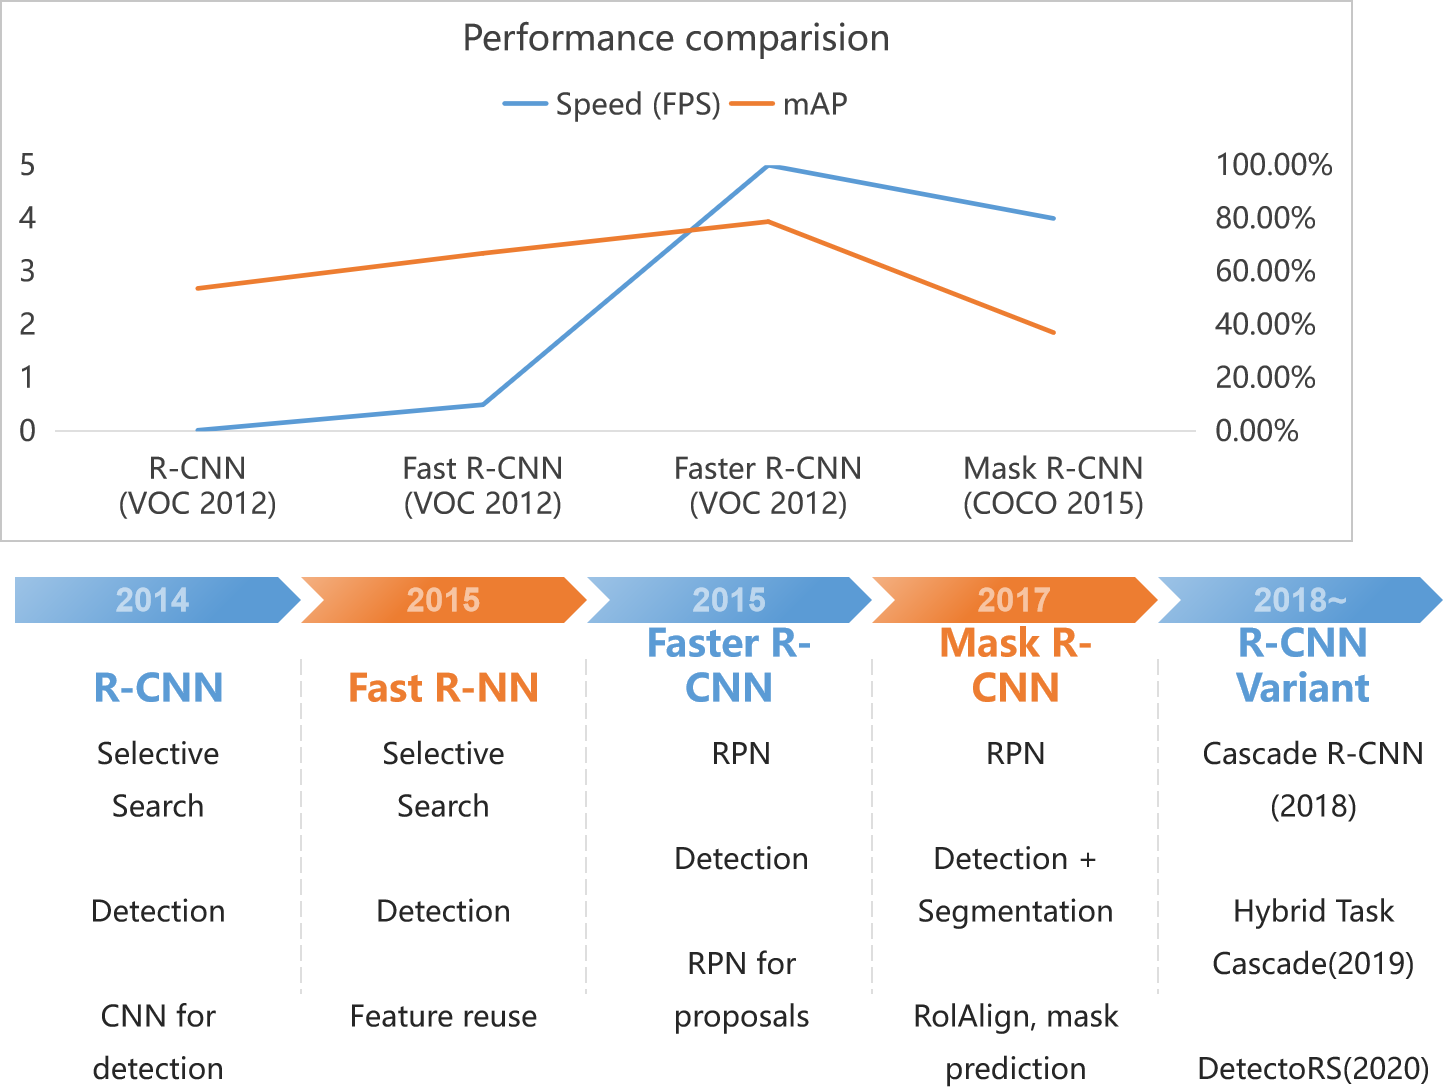
\includegraphics[width=0.5\textwidth]{fig_rcnn1.png}
\caption{The performance of R-CNN family for object detection.}
\label{fig:performance_rcnn}
\end{figure}

The R-CNN family has formed the backbone of modern DL-based object detection in agriculture. The original R-CNN, introduced in 2014~\cite{girshick2014rcnn}, pioneered the use of selective search to generate region proposals, followed by CNN-based feature extraction and SVM classification. Despite its improved detection accuracy, R-CNN's computational inefficiency—due to processing thousands of proposals per image—limited its real-time applicability.
To addressed these bottlenecks by sharing the convolutional computation across the entire image and using Region of Interest (RoI) pooling, Girshick~\cite{girshick2015fast} introduced Fast R-CNN in 2015, significantly expediting both training and inference. By sharing features across region proposals, it achieved a remarkable speed-up (e.g., ~2.3s/image compared to R-CNN's 47s/image) and higher accuracy (mean average precision (mAP) ~66.9\% on PASCAL VOC). However, it still relied on the time-consuming selective search for region proposal generation.
Subsequently, Ren et al. ~\cite{ren2015faster} presented Faster R-CNN in 2015, further integrated the detection pipeline by introducing a Region Proposal Network (RPN) directly within the convolutional architecture, which replaced selective search and enabled full end-to-end training. Faster R-CNN achieved a speed of ~0.2s/image and a mAP of ~78.8\% on PASCAL VOC, balancing speed and accuracy well. Despite its success, the RoI Pooling in Faster R-CNN introduced quantization errors. 
%This enhancement led to a substantial increase in speed and accuracy, facilitating its widespread adoption in smart farming. 
Later, Sa et al.~\cite{sa2016deepfruits} applied Faster R-CNN for multi-modal fruit detection, demonstrating its adaptability by fusing RGB and near-infrared data, resulting in robust performance under variable field conditions and reducing the annotation workload. Similarly, Wan et al.~\cite{wan2020faster} optimized Faster R-CNN with a self-learning image library and advanced data augmentation to improve detection speed and accuracy across multiple fruit types, achieving a mAP exceeding 91\%.
Recent research has extended Faster R-CNN to incorporate additional modalities and tailored architectures. Fu et al.\cite{fu2020faster} augmented the framework using RGB-D imaging for apple detection in dense orchards, while Tu et al.~\cite{tu2020passion} proposed a multi-scale Faster R-CNN variant (MS-FRCNN) for small passion fruit recognition, combining color and depth data to handle occlusions and illumination changes. Additional studies have demonstrated the efficacy of these advanced models for kiwifruit detection~\cite{fu2018kiwifruit}, improved detection in occluded and mixed scenarios~\cite{gene2019multi, mu2020intact}, and integration with radiometric data for enhanced performance in challenging environments.

\begin{figure}[hbtp]
\centering
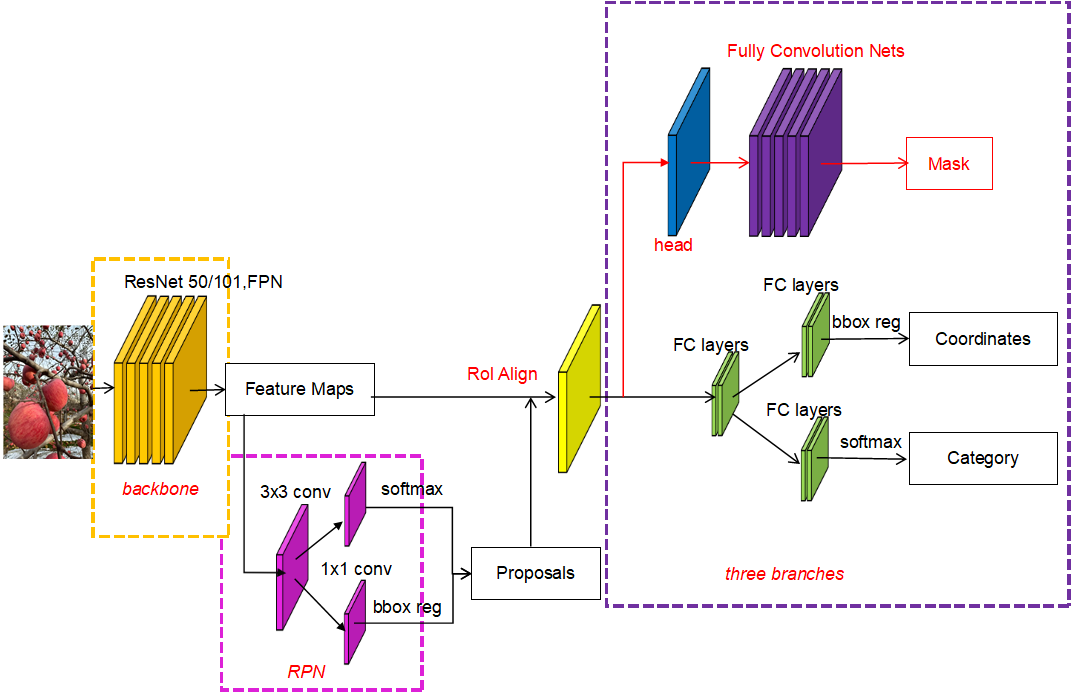
\includegraphics[width=0.5\textwidth]{fig_maskRcnn.png}
\caption{The Mask R-CNN process for object detection.}
\label{fig:mask_rcnn}
\end{figure}

\begin{table*}[htbp]
	\centering
	\footnotesize 
	\caption{Summary of R-CNN Family Approaches for Fruit Detection in 2015-2024} 
	\label{tab:RCNN-based} 
	\begin{tabular}{@{}p{0.4cm}p{0.4cm}p{1.4cm}p{1.8cm}p{2cm}p{1.8cm}p{2cm}p{4.3cm}@{}}
	\toprule
	\textbf{Ref.} & \textbf{Year} & \textbf{Fruit Type} & \textbf{Model Type} & \textbf{Main Gap} & \textbf{Performance} & \textbf{Datasets} & \textbf{Key Insights} \\ \midrule
\cite{sa2016deepfruits} & 2016 & Sweet Pepper, Rock Melon & Faster R-CNN & Multi-modal detection & F1: 0.838 & Commercial sites & Utilizes RGB and NIR; rapid deployment; explores early and late fusion methods \\ \midrule
\cite{wan2020faster} & 2023 & Multiple Fruits & Faster R-CNN & Multi-class detection & High precision & Custom Dataset & Uses depth features; real-time capable \\ \midrule
\cite{fu2020faster} & 2023 & Apples & Faster R-CNN & Dense foliage & AP 89.3\% & 700 field images & Depth features enhance detection \\ \midrule
\cite{tu2020passion} & 2023 & Passion Fruit & MS-FRCNN & Small fruit detection & F1-score 0.946 & RGB-D images & Effective at handling occlusions \\ \midrule
\cite{fu2018kiwifruit} & 2018 & Kiwifruit & Faster R-CNN with ZFNet & Detection in natural environments & AP 89.3\% & 2,100 sub-images & High precision under variable lighting; suitable for robotic harvesting \\ \midrule
\cite{gene2019multi}& 2021 & Fuji Apple & Multi-modal Faster R-CNN, RGB-D data, radiometric capabilities & Lack of multi-modal datasets, robust detection in varying conditions & F1-score: 0.898, AP: 94.8\% & KFuji RGB-DS dataset with 12,839 apples & Integration of radiometric data with RGB-D information enhances detection robustness \\ \midrule
\cite{mu2020intact} & 2020 & Tomato & Faster R-CNN with Resnet-101 & Occlusion and lighting variability & AP: 87.83\% ($IoU \geq 0.5$), $R^2 = 0.87$ & COCO & High accuracy in counting and location mapping \\ \midrule
\cite{yu2019fruit}& 2019 & Strawberry & Mask-RCNN & Non-structural detection & Precision 95.78\%, Recall 95.41\%, MIoU 89.85\% & 2000 images & Utilizes Mask-RCNN with ResNet50; high precision in picking point localization; effective in complex environments \\ \midrule
\cite{jia2020detection} & 2023 & Apples & Mask R-CNN & Overlapped fruits & High accuracy & Mixed orchard images & Optimized for segmentation \\ \midrule

\cite{chu2021deep} & 2021 & Apple & Suppression Mask R-CNN & Detection amidst occlusion & F1-score 0.905 & Custom orchard dataset & Novel suppression branch enhances accuracy \\ \midrule
\cite{gao2020multi} & 2020 & Apples & Faster R-CNN & Detection in SNAP systems & mAP: 0.879 & SNAP orchard images & Modified for small, occluded objects; real-time capable \\ \midrule
\cite{ge2019fruit} & 2019 & Strawberries & Mask R-CNN & High precision localization and collision avoidance & 74.1\% picking accuracy & Field tests & Advanced instance segmentation and environment perception enhance operational safety and efficiency in strawberry harvesting \\ \bottomrule
\end{tabular}
\end{table*}	

Despite the Faster R-CNN success, the RoI Pooling in Faster R-CNN introduced quantization errors. Mask R-CNN, proposed by He et al. ~\cite{he2017mask} in 2017, extended Faster R-CNN for instance segmentation. It introduced RoIAlign to improve spatial alignment and added a mask-prediction branch. Mask R-CNN achieved a mAP of ~37.1\% in segmentation and ~57.7\% in detection on MS COCO, but it was computationally more expensive.
Later, Cascade R-CNN was proposed by Cai et al. ~\cite{cai2018cascade} in 2018. It improved the detection of high-quality bounding boxes through a cascade of detectors with increasing IoU thresholds, achieving a higher mAP (e.g., 42.8\% on COCO) at the cost of some speed. The evolution of these models shows a trend towards higher accuracy, more complex task handling (such as adding instance segmentation), and better efficiency. Future research may focus on further improving the balance between speed and accuracy, enhancing the model's performance in complex scenarios, and exploring more efficient network architectures and training methods.
Hybrid Task Cascade (HTC) was introduced by Chen et al.~\cite{chen2019hybrid} in 2019. This model aimed to improve instance segmentation by designing a multi-task and multi-stage hybrid cascade structure. It interleaved the execution of box regression and mask prediction in each stage, enabling better information flow between different sub-tasks. Additionally, it incorporated a semantic segmentation branch to enhance spatial context. HTC achieved a mAP of 48.2\% in detection and 43.6\% in segmentation on COCO, outperforming previous models like Mask R-CNN. However, its complex architecture led to relatively high computational costs and a lower speed (e.g., 2.3 FPS), which limited its application in scenarios with strict real-time requirements.
DetectoRS, proposed by Qiao et al. ~\cite{qiao2021detectors} in 2020, was designed to address issues such as multi-scale feature fusion and insufficient receptive fields. It employed a recursive feature pyramid and switchable atrous convolution. This approach significantly improved the model's ability to handle objects of different scales, achieving a mAP of 52.8\% in detection on COCO. Despite its high accuracy, DetectoRS was computationally expensive and had a relatively low speed (e.g., 1.9 FPS) due to its complex network design.
Following these advancements, subsequent research has focused on developing more lightweight architectures, improving the balance between speed and accuracy, and enhancing the models' generalization ability in diverse and complex real-world scenarios. For example, some studies explore the use of more efficient backbone networks or novel attention mechanisms to reduce computational load while maintaining high-level performance.
Yu et al.~\cite{yu2019fruit} employed Mask R-CNN for robust strawberry segmentation in the field, achieving an average precision above 95\% despite varied lighting and occlusions. Further model refinements such as the incorporation of feature pyramid networks and improved backbone architectures have enabled effective contour and picking point detection for strawberries~\cite{jia2020detection} and apples~\cite{chu2021deep}, with each study reporting improvements in segmentation accuracy, F1-scores, and false positive reduction. Ge et al.~\cite{ge2019fruit} leveraged Mask R-CNN for environmental scene understanding and obstacle avoidance in strawberry harvesting, demonstrating enhanced robotic safety and efficiency.

%Table~\ref{tab:rcnn_comparison} 
Figure~\ref{fig:performance_rcnn} provides a detailed comparative overview of R-CNN, Fast R-CNN, Faster R-CNN, and Mask R-CNN, outlining their advancements in proposal generation, feature extraction, computational efficiency, and detection capabilities. The continuous improvement of these frameworks has addressed the fundamental challenges of detection speed and accuracy, driven the transition from bounding box localization to instance-level segmentation, and directly enabled the development of state-of-the-art fruit-picking robots for complex agricultural settings.




\subsection{YOLO Series}
After exploring the applications of R-CNN family models in fruit picking, another prominent research direction in the field of computer-vision-enabled agricultural automation is the YOLO series as illustrated in Figure~\ref{fig:yolo}. While the R-CNN family emphasizes iterative refinement and multi-stage processing, YOLO's single-stage detection framework offers real-time performance, making it an attractive alternative for dynamic fruit-picking scenarios.
\begin{figure}[hbtp]
\centering
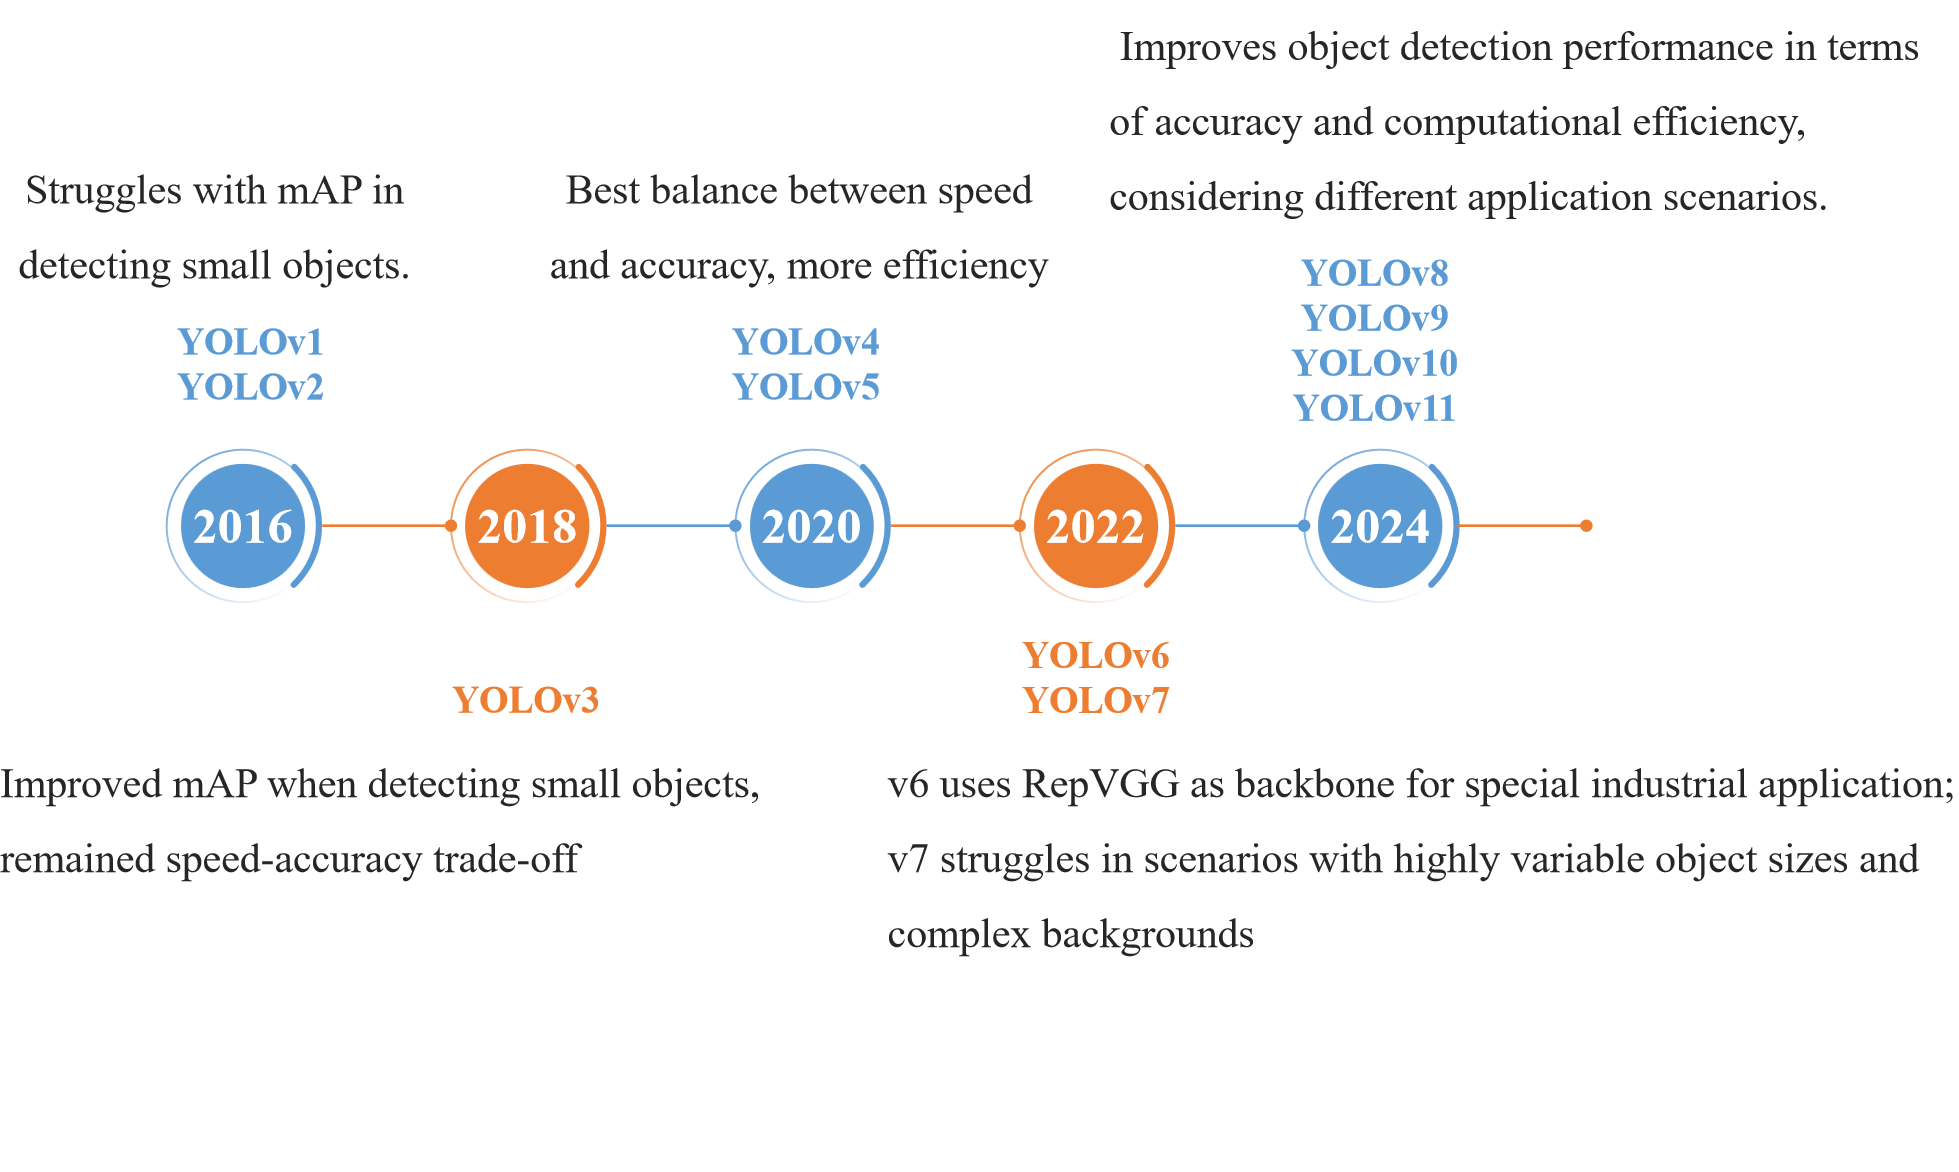
\includegraphics[width=0.5\textwidth]{fig_yolo.png}
\caption{The YOLO Series Roadmap.}
\label{fig:yolo}
\end{figure}

In recent years, YOLOv3~\cite{redmon2018yolov3}, YOLOv4~\cite{bochkovskiy2020yolov4}, and YOLOv5 have emerged as the dominant choices for fruit-picking applications. YOLOv3 introduced the Darknet-53 backbone and multi-scale prediction, enabling more accurate detection of small fruits obscured by leaves. YOLOv4 further optimized performance by integrating techniques like Cross Stage Partial Darknet53 (CSPDarknet53) and Complete Intersection over Union (CIoU) loss, striking a balance between speed and accuracy suitable for real-time robotic operations. YOLOv5, initially released as an open-source project by Ultralytics (without a traditional academic paper in the same format as others) has a modular design with customizable scales (e.g., n, s, m, l, x) allows researchers to tailor the model for different hardware constraints in the orchard, from edge devices on robotic arms to onboard GPUs. However, their reliance on traditional feature extraction and post-processing limits performance in highly occluded or low-light environments common in orchards.
Conversely, YOLOv6~\cite{li2022yolov6} and YOLOv7~\cite{wang2023yolov7} encounter difficulties when adapting to direct fruit picking. YOLOv6 has been designed with industrial assembly line scenarios in mind. It employs a Re-parameterized VGG (RepVGG) model to facilitate inference-time acceleration.  However, it encounters challenges when confronted with fruits of irregular poses and complex backgrounds. 
Despite its advanced Extended-efficient-layer aggregation networks (ELAN) architecture and  "bag-of-freebies" trainable, YOLOv7 demands substantial computational resources which conflicts with the power constraints of most fruit-picking robots. It is evident that both of these systems necessitate optimisations that are specific to the agricultural domain. 
The most recent iterations of YOLO (v8-v11)~\cite{yaseen2024yolov9, wang2024yolov10, khanam2410yolov11}, present promising directions but remain in the exploratory phase for fruit-picking. demonstrate potential but remain in the exploratory stage. The YOLOv8 model facilitates multitasking capabilities, encompassing operations such as object detection, instance segmentation, and classification, thereby enabling the concurrent identification of fruit ripeness. YOLOv9's Generalized Efficient Layer Aggregation Network (GELAN) and Programmable Gradient Information (PGI) enhance feature extraction across fruit scales, potentially improving detection of clustered or differently-sized fruits. It is evident that YOLOv10's NMS has the capacity to reduce inference latency. YOLOv11's Spatial Pyramid Pooling Fast (SPPF) and Convolutional Block with Parallel Spatial Attention (C2PSA) components improve attention to occluded fruits, albeit with an attendant increase in task complexity.
%Currently, most research on YOLOv8 - v11 focuses on general object detection in autonomous driving, surveillance, and industrial inspection, where abundant computational resources and controlled data distributions facilitate rapid model development. In fruit picking, although initial studies have demonstrated improved detection rates for specific fruit types, challenges persist. These include handling diverse weather conditions, adapting to varying fruit growth patterns, and ensuring reliable operation on resource - constrained robotic platforms. As such, while YOLOv8 - v11 represent the cutting - edge of object - detection technology, their full integration into fruit - picking systems requires further optimization, validation across multiple crop types, and real - world deployment testing, solidifying their status as a critical research frontier in agricultural robotics.

%The YOLO family of algorithms represents a critical advancement in real-time object detection, with broad adoption in agricultural robotics, particularly for fruit-picking applications. The principal advantage of YOLO is its speed: the framework processes entire images in a single neural network pass, predicting bounding boxes and class probabilities concurrently. This attribute makes it exceptionally well-suited for scenarios requiring rapid and reliable detection, such as autonomous harvesting.
%The evolution of the YOLO series has seen continual enhancement in detection performance, model efficiency, and adaptability to complex environments. YOLOv3 introduced multi-scale feature detection, improving the identification of small and variably sized fruit objects within dense canopies, a frequent challenge in orchard environments. Further, YOLOv4 delivered improvements in accuracy and computational speed by integrating architectural advancements such as the CSPDarknet53 backbone, PANet path aggregation, and optimized anchor box selection. While YOLOv5 is not an official release from the original authors, it has gained substantial traction in the research community due to its user-friendly implementation, fast training times, and lightweight architecture, making it a popular choice for deployment on resource-constrained agricultural platforms.


Empirical research underscores the practical impact and versatility of the YOLO series in horticultural and orchard automation. For example, Liu et al.~\cite{liu2020yolo} proposed an improved YOLOv3 architecture (YOLO-Tomato) tailored for robust tomato detection under variable lighting and occlusion, demonstrating high precision and field applicability. Lawal~\cite{lawal2021tomato} presented further enhancements to YOLOv3 for tomato detection, offering improved accuracy and operational speed that meet real-time harvesting requirements.
Complex fruit environments often require specialized modifications. Gai et al.~\cite{gai2023detection} advanced detection for cherries by integrating DenseNet modules into an improved YOLOv4 model and introducing a circular bounding box approach, significantly boosting performance under challenging lighting and occlusion. Similarly, Kuznetsova et al.~\cite{kuznetsova2020using} demonstrated that pre- and post-processing strategies improve YOLOv3 performance for apples in natural orchards by effectively addressing issues of varying lighting and object obstruction.
Lightweight models within this family are particularly important for real-time deployment. Magalhães et al.~\cite{magalhaes2021evaluating} systematically evaluated SSD MobileNet v2 and YOLOv4 Tiny for greenhouse tomato detection, confirming their suitability for integration with autonomous harvesting machinery and for mitigating the costs associated with manual agricultural labor. Li et al.~\cite{li2021real} further modified the YOLOv4-Tiny model (YOLO-Grape) for grape detection by incorporating depthwise separable convolutions, attention mechanisms, and the Mish activation function, achieving an F1-score of 90.47\% and real-time detection speeds suitable for orchards with complex backgrounds.
Several studies have explored integrating these detection algorithms with complementary vision and robotic technologies. Tang et al.~\cite{tang2023fruit} enhanced the YOLOv4-Tiny framework with k-means++ clustering and additional convolutional layers, utilizing binocular stereo vision to support precise fruit localization in orchards. Sozzi et al.~\cite{sozzi2022automatic} compared the efficacy of multiple YOLO models for white grape detection, demonstrating that YOLOv4 and YOLOv5 deliver superior accuracy and speed, which is essential for vineyard yield estimation and management.
Earlier breakthroughs include Bresilla et al.~\cite{bresilla2019single}, who applied a modified YOLO architecture for real-time detection of apples and pears within tree canopies, achieving accuracy rates above 90\% at over 20 frames per second. This work confirmed the feasibility of deploying DL-based detection for efficient automated harvesting. Jun et al.~\cite{jun2021towards} developed a tomato-harvesting robot that combined the YOLOv3 detection model with RGB-D sensors for three-dimensional localization, paired with a specialized end-effector, resulting in a detection precision of 95\% and efficient harvest cycles in laboratory experiments.

Overall, the YOLO series has significantly contributed to real-time object detection and localization in agricultural robotics. The adaptations and continual improvements across YOLOv3, YOLOv4, and YOLOv5 have addressed core challenges such as detecting small or occluded fruit, optimizing inference for dense foliage, and maintaining computational efficiency in the field. Table~\ref{tab:yolo-based} provides a comparative overview of different YOLO versions, illustrating the specific enhancements that advance their suitability for diverse, real-world agricultural environments. These developments collectively promote both the reliability and scalability of autonomous fruit-picking systems.

\begin{table*}[H]
	\centering
	\footnotesize 
	\caption{Summary of YOLO Family Approaches for Fruit Detection since 2019} 
	\label{tab:yolo-based} 
	\begin{tabular}{p{0.03\linewidth} p{0.03\linewidth} p{0.06\linewidth} p{0.06\linewidth} p{0.12\linewidth} p{0.12\linewidth} p{0.12\linewidth} p{0.28\linewidth}}
	\toprule
	\textbf{Ref.} & \textbf{Year} & \textbf{Fruit Type} & \textbf{Model Type} & \textbf{Main Gap} & \textbf{Performance} & \textbf{Datasets} & \textbf{Key Insights} \\ \midrule
\cite{liu2020yolo}  & 2021 & Tomato & YOLOv3 & Detection across growth stages & Effective in complex environments & Farming environments & Optimized for agricultural applications, real-time capable \\ \midrule
\cite{lawal2021tomato} & 2023 & Tomatoes & Modified YOLOv3 & Greenhouse environment & SSD MobileNet v2 top performer & Greenhouse dataset & Compares SSD and YOLO models \\ \midrule
\cite{gai2023detection} & 2023 & Cherries & Improved YOLO-v4 & Detection in varying conditions & High AP & Controlled conditions & Enhanced with DenseNet; circular bounding boxes \\ \midrule
\cite{kuznetsova2020using} & 2023 & Apples & YOLOv3 & Pre-/Post-Processing & High efficiency & Orchard dataset & Advanced pre-/post-processing \\ \midrule
\cite{magalhaes2021evaluating} & 2023 & Tomatoes & YOLO & Greenhouse accuracy & Superior detection & Controlled conditions & Improved accuracy and speed \\ \midrule
\cite{li2021real} & 2023 & Grapes & YOLOv4-Tiny & Complex background & F1-score 90.47\% & Vineyard images & Real-time, low computational cost \\ \midrule
\cite{tang2023fruit} & 2023 & Camellia oleifera & YOLOv4-Tiny & Precise positioning & AP 92.07\% & Orchard dataset & Combines DL with stereo vision \\ \midrule
\cite{sozzi2022automatic} & 2023 & White Grapes & YOLOv3, YOLOv4, YOLOv5 & Bunch detection & Best F1-score 0.77 & Vineyard dataset & Effective in vineyard settings \\ \midrule
\cite{jun2021towards} & 2021 & Tomatoes & YOLOv3 with RGB-D sensors & Accurate and efficient harvesting in greenhouses & 95\% detection precision; 5.9 seconds per tomato & 770 images from greenhouse environment & Combines 3D perception and a novel end-effector design to enhance efficiency and reduce fruit damage during harvesting. \\ \midrule
\cite{yu2020real} & 2020 & Strawberry & R-YOLO & Localization in narrow spaces & Recognition rate 94.43\%, Recall 93.46\% & Ridge-planting strawberry fields & Utilizes rotated YOLO for precise localization; optimizes real-time performance on embedded systems \\  \midrule
\cite{bresilla2019single}& 2019 & Apples, Pears & Modified YOLO & Real-time detection in complex backgrounds & Over 90\% accuracy, 20+ FPS & Orchard images & Optimizes YOLO for fast, accurate fruit detection suitable for robotic harvesting \\  \midrule
\cite{yu2024object} & 2024 & Citrus & Improved YOLOv5 & Leaf occlusion, overlapping fruits, and variable lighting conditions  &  A high detection precision of 95.83\% and a mAP of 79.68\% & Orchard dataset & Enhanced the YOLOv5 model by introducing receptive field convolutions with full 3D weights (RFCF), addressing the limitations from parameter sharing in traditional convolution operations and thus improving detection accuracy.. \\ \midrule  
\cite{ZHOU2024110} & 2024 & \textit{C. oleifera} & YOLOv8x & 3D positioning for robotic harvesting & mAP50: 0.96 & Annotated \textit{C. oleifera} dataset (1012) & Integration of depth cues with advanced 2D detection delivers sub-centimeter positioning accuracy for harvesting robots. \\ \midrule 
\cite{ZHANG2024108780} & 2024 & Fruit tree trunks & Improved YOLOv5 & Trunk detection for orchard operation robots & mAP: 97.1\% & Natural orchard (1354 images) & Hybrid attention modules bolster trunk recognition under variable illumination and occlusion conditions. \\ \midrule  
\cite{ZHANG2024108836} & 2024 & Citrus & MFAF-YOLO & Real-time detection in complex citrus orchards & mAP: 90.2\%, AP (First priority): 93.2\%, AP (Second priority): 87.3\% & Real-field citrus images & Multi-frequency attention mechanisms dynamically adapt to different citrus growth stages and environmental conditions. \\ \midrule  
\cite{LU2024108721} & 2024 & Citrus & Yolo-FD & Citrus peel defect and fruit morphology detection & mAP: 98.7\%, Morphology Accuracy: 91.42\% & N/A & Dual-branch design enables simultaneous defect detection and morphological analysis for enhanced quality control. \\ \bottomrule
\end{tabular}
\end{table*}

\subsection{Fruit Segmentation}
Recent advancements in DL have notably improved fruit detection and segmentation, addressing longstanding challenges in agricultural robotics such as varying lighting, occlusion, and complex backgrounds. Through continual development and the adaptation of neural network architectures, segmentation networks now support enhanced autonomy and operational performance in fruit-picking robots.

Initial efforts in fruit segmentation largely relied on color, shape, and edge features. For instance, Lu and Sang~\cite{lu2015detecting} developed a technique for detecting citrus fruits under natural light using color properties, contour fragments, and ellipse fitting to robustly segment and identify fruit despite occlusion. Liu et al.~\cite{liu2016method} proposed a two-stage apple segmentation method combining color and positional information to enable accurate night-time detection. Lehnert et al.~\cite{lehnert2016sweet} utilized color segmentation and 3D clustering to estimate the pose of sweet peppers, enabling precise robotic grasping with a 6-DOF manipulator. Wang et al.~\cite{wang2017robust} enhanced segmentation robustness under variable illumination by combining wavelet-based normalization, Retinex image enhancement, and K-means clustering, thereby improving overall detection accuracy.
With the progress of DL, CNNs and fully convolutional architectures became mainstream. Peng et al.~\cite{peng2018general} improved the SSD model by integrating ResNet-101 with the SSD framework to detect multiple fruit types in open environments. This adaptation resulted in high detection accuracy and efficiency, with an average accuracy of 89.53\% and an F1-score of 96.12\%. Barth et al.~\cite{barth2018data} contributed a synthetic dataset approach for semantic segmentation of Capsicum annuum using procedurally modeled imagery, demonstrating significant gains in data augmentation and model generalizability.
Lin et al.~\cite{lin2019guava} and Lin et al.~\cite{lin2020color} advanced the field by using low-cost RGB-D sensors and fully convolutional networks for guava detection and 3D pose estimation. These systems delivered high accuracy in fruit segmentation and localization with rapid processing, supporting practical implementation in resource-constrained environments.

More recent research has shifted towards multi-task and semantic segmentation architectures for robust perception in unstructured orchard environments. Kang and Chen~\cite{kang2019fruit, kang2020fruit} introduced the DaSNet and DaSNet-v2 models, employing ResNet backbones and Gated Feature Pyramid Networks for simultaneous detection and semantic segmentation of fruits and branches. Their systems achieved high F1-scores and demonstrated ability to handle complex orchard scenes, providing 3D environmental visualizations critical for autonomous navigation and harvesting. Majeed et al.~\cite{majeed2020deep} applied the SegNet architecture for semantic segmentation of apple tree canopies, facilitating tasks such as trunk, branch, and trellis identification to automate orchard management and training processes.
For specific crop types, Birrell et al.~\cite{birrell2020field} presented Vegebot, a robotic harvester for iceberg lettuce, integrating advanced vision with robotic manipulation to achieve a 91\% localization rate in field conditions. Luo et al.~\cite{luo2018vision} developed a vision-based methodology that accurately detects cutting points on grape peduncles, overcoming the occlusion and variability of vineyards, achieving an average accuracy of 88.33\%.

Semantic segmentation with models such as DeepLabV3 and U-Net further refined perception in agricultural robotics. Peng et al.~\cite{peng2020semantic} optimized DeepLabV3 with the Xception65 backbone for litchi branch segmentation, reporting a mean intersection-over-union of 0.765; Li et al.~\cite{li2020detection} and Li et al.~\cite{li2021novel} extended semantic segmentation for litchi and green apples using RGB-D data, ensemble U-Net models, edge structures, and gated convolutions, achieving high accuracy in complex, real-world orchard environments.
Pereira et al.~\cite{pereira2019deep} focused on the identification of grape plant species via transfer learning and AlexNet, successfully distinguishing visually similar varieties under challenging conditions with test accuracies up to 89.75\%. Rahnemoonfar and Sheppard~\cite{rahnemoonfar2017deep} introduced "Deep Count"—a synthetic data-driven fruit counting network, achieving 91\% accuracy, illustrating the value of artificial datasets in overcoming ground truth limitations.

Combining segmentation with contemporary detection algorithms has further improved system robustness. Luo et al.~\cite{luo2016robust} combined AdaBoost and color component analysis for resilient grape detection in unstructured settings. Kirk et al.~\cite{kirk2020b} integrated bio-inspired features and the CIELab color space into a RetinaNet model to enhance strawberry detection under variable lighting, achieving superior F1-scores compared to traditional approaches. Peng et al.\cite{peng2018general} and Feng et al.~\cite{feng2018} demonstrated that integrating classic image processing (edge detection, color segmentation) with DL yields high accuracy for challenging targets such as cherry tomato bunches.

The ongoing evolution from rule-based methods to advanced deep segmentation networks—with domain adaptation, multi-task learning, and synthetic data augmentation—has markedly advanced the accuracy, efficiency, and autonomy of robotic fruit detection and harvesting systems. These approaches address the primary challenges of real-world agricultural environments, setting new standards for performance and practical adoption in precision agriculture.

\subsection{Challenges-Oriented Solutions and Applications}
The practical deployment of fruit-picking robots faces several challenges, focused on the Precision, Rapidity and Reliability as illustrated in Figure~\ref{fig:performance}. Researchers have proposed various solutions to address these challenges.
Fruit picking-point detection in agricultural robotics typically involves identifying where the fruit attaches to the plant, which is crucial for effective and damage-free harvesting. The algorithms used for this purpose often include image segmentation techniques, edge detection, Geometric and Morphological Features, and ML models.
Image Segmentation techniques separate different parts of the plant based on color, texture, or depth information. For example, the stem of sweet peppers can often be distinguished from the fruit and leaves by its distinct color and texture characteristics.
Once the regions of interest (e.g., potential stem areas) are segmented, edge detection algorithms might be applied to outline the precise boundaries of the stem, which can help pinpoint the exact location where the fruit connects to the stem.
Algorithms might analyze detected objects' geometric shapes and morphological features to identify stem-like structures, which could involve detecting elongated, cylindrical shapes typical of stems among the rounded shapes of fruits. Advanced implementations might train ML models, particularly CNNs, on labeled images to learn and accurately predict the location of stems.
\begin{figure}[hbtp]
\centering
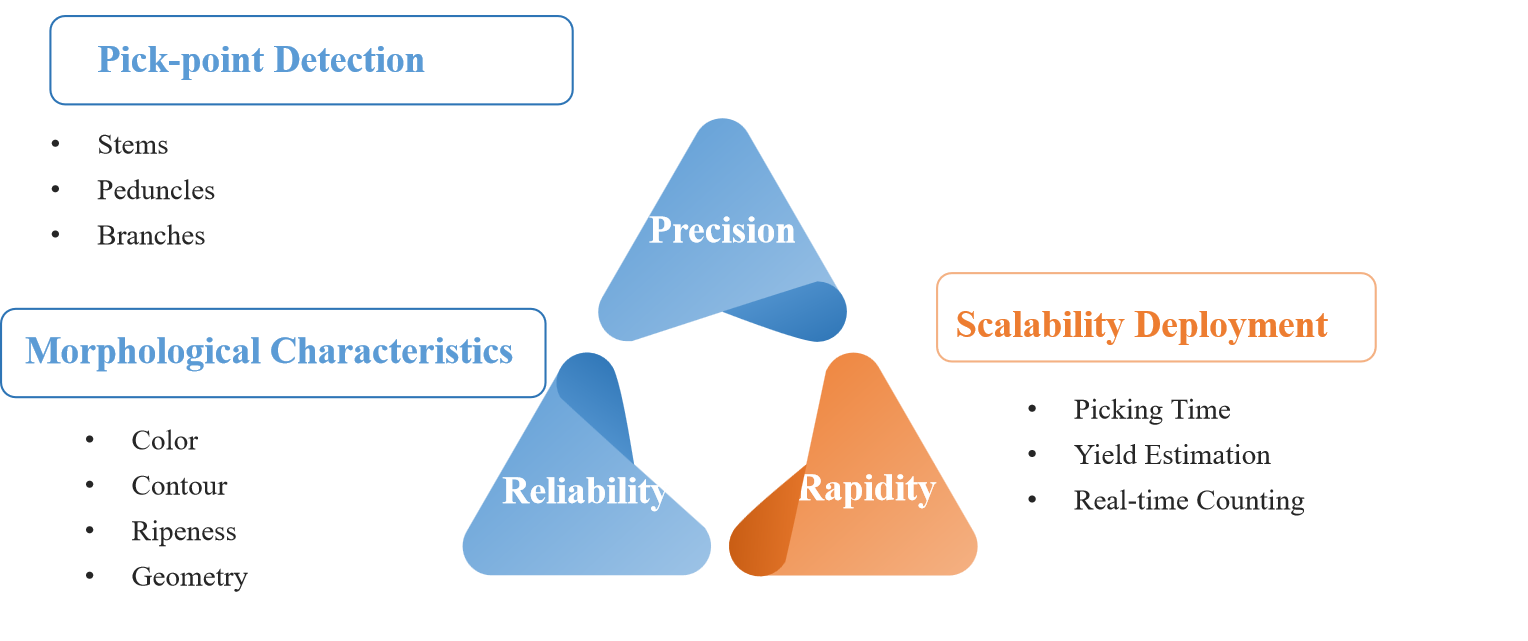
\includegraphics[width=0.5\textwidth]{fig_performance.png}
\caption{The Challenges-Oriented Solutions.}
\label{fig:performance}
\end{figure}
Accurate pick-point detection is fundamental to the success of autonomous fruit and vegetable harvesting. Progress in this area has focused on identifying critical structural features, such as stems, peduncles, branches, and optimal cutting points, under varying environmental and crop-specific challenges.
Bac et al.~\cite{bac2017performance} enhanced stem detection reliability by incorporating multispectral imaging and artificial lighting, alongside advanced algorithms that exploit both color and textural differences. This method enabled the robotic system to achieve precise cutting with minimal damage to crops, demonstrating the value of sensor fusion and image enhancement in complex plant structures.
In vineyard applications, Mendes et al.~\cite{mendes2016vine} developed ViTruDe, an advanced visual detection system for the robust identification of vine trunks and masts in situations where GPS is unreliable. By employing techniques such as Sobel keypoint detection, Local Binary Pattern (LBP) region descriptors, and SVM classification, the system achieved greater than 95\% accuracy, thereby enabling precise autonomous navigation and further highlighting the potential of vision-based approaches in challenging agricultural terrains.

Detection of fruit peduncles is critical for minimizing crop damage during harvesting. Sa et al.~\cite{sa2017peduncle} proposed a 3D visual detection method utilizing the combined information from RGB-D sensors, incorporating both color and geometry to identify sweet pepper peduncles. The method achieved a detection area under the curve (AUC) of 0.71 for the precision-recall curve and significantly outperformed color-only techniques, validated on a manually annotated dataset for sweet pepper peduncles.
Luo et al.~\cite{luo2018vision} developed a vision-based approach to detect cutting points on peduncles of grape clusters in complex vineyard environments. By addressing the challenges of overlapping fruits and unstructured conditions, their method achieved an average recognition accuracy of 88.33\% and a success rate of 81.66\% for cutting point localization, demonstrating tangible benefits for robotic grape harvesting.
Yu et al.~\cite{yu2020real} addressed the practical need for real-time pick-point localization in strawberry harvesting. Their R-YOLO architecture employs rotated bounding boxes and MobileNet-V1 for lightweight, rapid feature extraction. Operating at 18 frames per second on embedded hardware, the system identifies optimal strawberry picking points in ridge-planting scenarios with a recognition rate exceeding 94\%, substantially improving picking efficiency and accuracy under authentic agricultural conditions.
Pérez-Zavala et al.~\cite{perez2018pattern} presented a robust vision strategy for grape bunch detection using standard RGB cameras under natural illumination. By integrating Histogram of Oriented Gradients (HOG) for shape and LBP for texture extraction with SVM classification, the approach achieved 88.61\% precision and 80.34\% recall, demonstrating adaptability across grape cultivars and lighting variations, thus supporting practical automated viticulture.

%Collectively, these studies illustrate the progressive refinement of pick-point detection approaches, addressing the diverse requirements of crop types, harvesting scenarios, and environmental complexities. Advanced sensor integration, robust machine vision algorithms, and tailored network architectures have fundamentally improved the reliability and safety of autonomous harvesting systems, driving practical deployment in both protected and open-field agriculture.

The deployment of real-time machine vision systems is a pivotal factor driving the automation and efficiency of agricultural harvesting operations. Recent years have seen substantial progress in the development and application of robust computer vision, ML, and DL methods that fulfill the stringent requirements of agricultural environments, delivering reliable, rapid, and scalable solutions for fruit detection, grading, and harvesting.
Goel and Sehgal~\cite{goel2015fuzzy} proposed a fuzzy rule-based classification system for tomato ripeness estimation, leveraging color feature extraction and a decision tree learning algorithm. Their approach enables rapid and accurate classification of tomatoes into six maturity stages (94.29\% accuracy) using images captured under natural light, reducing subjectivity and labor in the ripening assessment process.
Zhao et al.~\cite{zhao2016robust} advanced tomato recognition for low-cost robotic platforms by fusing features from multiple color spaces, employing the Lab* a*-component and YIQ I-component with wavelet transformation to address illumination variability and occlusion. Their system maintained a recognition rate of 93\% in field tests, demonstrating the reliability of feature fusion techniques for robust, real-time detection.
Lin et al.~\cite{lin2019field} developed a real-time citrus detection and localization approach utilizing RGB-D imaging coupled with depth filtering, density clustering, and SVM classification. Achieving an F1 score of 0.9197 under conditions of variable lighting and partial occlusion, this method improved feasibility for automated orchard harvesting.
Wang L L et al.~\cite{lili2017development} engineered a comprehensive robotic system for greenhouse tomato harvesting, integrating a binocular stereo vision module, laser navigation, and four-wheel steering for efficient mobility. The system delivered high recognition accuracy and precise navigation, illustrating the convergence of multi-modal sensing and motion planning to enhance operational efficiency in dense crop environments.

DL and efficient model architectures have significantly upgraded real-time fruit classification capabilities. Xiang et al.~\cite{xiang2019fruit} deployed MobileNetV2, combined with transfer learning, for lightweight, rapid fruit sorting, achieving 85.12\% accuracy on a heterogeneous dataset and demonstrating practical viability for low-power agricultural devices. Altaheri et al.~\cite{altaheri2019date} automated date fruit classification by fine-tuning AlexNet and VGGNet through transfer learning, attaining high classification accuracy and speeds compatible with real-time robotic harvesting in orchard environments.
Mao et al.~\cite{mao2020automatic} proposed a multi-feature fusion cucumber recognition algorithm, combining a Multi-Path Convolutional Neural Network (MPCNN) and selective color component analysis. Supported by SVM classification, their approach achieved rapid, high-accuracy detection and proved effective in complex, open-field settings, furthering the development of autonomous harvesting systems.
Barth et al.~\cite{barth2016design} presented a modular software framework designed for robust robotic harvesting in dense crop scenarios, integrating eye-in-hand sensing, visual servo control, and scene reconstruction within the Robot Operate System (ROS) ecosystem. Validated on a synthetic sweet-pepper crop, the system displayed adaptability and efficiency for automated operations in high-density vegetation.
Kang et al.~\cite{kang2020real} further advanced real-time operational efficiency by integrating a DL-based detection module (Mobile-DasNet) with PointNet-based grasp estimation in a robotic apple harvesting system. This configuration enabled precise and reliable picking under various environmental conditions, highlighting the practical benefits of deep network architectures in agricultural robotics.

\begin{table*}[htbp]
	\centering
	\footnotesize 
	\caption{Summary of Other Segmentation Approaches for Fruit Detection in 2015-2024(Part 1)} 
	\label{tab:machinelearning-based} 
	\begin{tabular}{@{}p{0.4cm}p{0.4cm}p{1.4cm}p{1.4cm}p{2cm}p{2cm}p{2cm}p{4.5cm}@{}}
	\toprule
	\textbf{Ref.} & \textbf{Year} & \textbf{Fruit Type} & \textbf{Model Type} & \textbf{Main Gap} & \textbf{Performance} & \textbf{Datasets} & \textbf{Key Insights} \\ \midrule
\cite{rahnemoonfar2017deep} & 2017 & Various fruits & Inception-ResNet & Counting without detection & 91\% on real images & Synthetic and real images & Utilizes synthetic data; robust to occlusion and variable lighting \\  \midrule
\cite{luo2018vision} & 2018 & Grapes & Vision-based detection & Cutting point detection in overlapping clusters & Recognition accuracy 88.33\%, Success rate 81.66\% & Vineyard images & Integrates k-means clustering and geometric analysis for precise cutting point detection in complex environments \\  \midrule
 \cite{lin2019guava} & 2019 & Guava & FCN + 3D line-segments & Real-time field detection & Precision 0.983, Recall 0.948 & Outdoor guava orchard & Integrates RGB-D sensing with FCN for accurate fruit detection and pose estimation; suitable for robotic applications \\ \midrule
\cite{mendes2016vine} & 2016 & Vine trunks & ViTruDe & Localization in GPS-denied areas & Over 95\% accuracy & Vineyard settings & Employs Sobel operator and SVM for robust trunk and mast detection in vineyards \\ \midrule
\cite{kang2020fruit} & 2020 & Apples & DaSNet-v2 & Real-time performance in complex environments & Recall 0.868, Precision 0.88, Branch Seg. Acc. 0.794 & Apple orchards & Advanced instance and semantic segmentation for real-time robotic harvesting \\ \midrule
\cite{lin2020color} & 2020 & Multiple fruits & MSAC + SVM & Robust universal detection & Precision: Peppers 0.864, Eggplants 0.886, Guavas 0.888; Recall: Peppers 0.889, Eggplants 0.762, Guavas 0.812 & Field datasets & Integrates color, depth, and shape for precise fruit detection; employs advanced image segmentation and 3D shape detection techniques \\ \midrule
\cite{barth2018data} & 2018 & Sweet pepper & Semantic segmentation with synthetic data & Overcoming data scarcity in agriculture & Enhanced model training and refinement & 10,500 synthetic images & Developed a comprehensive synthetic dataset for training agricultural vision systems; integrated synthetic and empirical data for effective model refinement. \\ \midrule
\cite{zhao2016detecting} & 2016 & Tomatoes & AdaBoost + Color Analysis & Robust detection in complex backgrounds & Detected over 96\% of ripe tomatoes, False negative rate ~10\% & Greenhouse images & Combines AdaBoost and color analysis for enhanced accuracy in detecting tomatoes in variable greenhouse environments \\ \midrule
\cite{lin2020fruit} & 2019 & Multiple fruits & PSM + PHT + SVM & Contour-based detection in natural settings & High effectiveness across various fruits & Citrus, tomato, pumpkin, etc. & Innovates with contour-based detection overcoming low contrast and illumination issues \\  \midrule
\cite{majeed2020deep} & 2020 & Apples & SegNet & Automated training in orchards & High accuracies for trunks (0.91), branches (0.92), and wires (0.97) & RGB and depth data from Kinect V2 & Utilizes DL for precise segmentation and automated training, reducing labor in orchards \\ \midrule
\cite{altaheri2019date}  & 2019 & Dates & AlexNet, VGGNet & Real-time classification in natural environments & Type: 99.01\%, Maturity: 97.25\%, Harvest: 98.59\%; Fast classification times & Over 8000 images of diverse date types and maturity stages & Pioneers in applying DL for real-time date fruit classification, enhancing robotic harvesting efficiency \\  \midrule
\cite{kang2020real}  & 2020 & Apples & Mobile-DasNet, PointNet & Integration of detection and grasping & High success rate; 6.5s cycle time & Laboratory and orchard tests & Demonstrates effective real-time fruit recognition and robotic grasping, enhancing automated apple harvesting \\ \midrule
\cite{goel2015fuzzy} & 2015 & Tomatoes & FRBCS, Decision Trees & Accurate ripeness assessment & 94.29\% accuracy & Field images & Utilizes fuzzy logic and decision trees to classify tomato ripeness with high accuracy, enhancing pre-harvest decision-making \\  \midrule
\end{tabular}
\end{table*}

\begin{table*}[htbp]
	\centering
	\footnotesize 
	\addtocounter{table}{-1}
	\caption{Summary of Other Segmentation Approaches for Fruit Detection in 2015-2024(Part 2)} 
	\label{tab:machinelearning-based} 
	\begin{tabular}{@{}p{0.4cm}p{0.4cm}p{1.4cm}p{1.4cm}p{2cm}p{2cm}p{2cm}p{4.5cm}@{}}
	\toprule
	\textbf{Ref.} & \textbf{Year} & \textbf{Fruit Type} & \textbf{Model Type} & \textbf{Main Gap} & \textbf{Performance} & \textbf{Datasets} & \textbf{Key Insights} \\ \midrule
\cite{zhao2016robust} & 2016 & Tomatoes & Image Fusion (Wavelet) & Complex environments & 93\% recognition rate & Field images & Combines a*- and I-component image fusion via wavelet transformation for robust tomato detection in variable conditions. \\ \midrule
\cite{mao2020automatic} & 2020 & Cucumbers & MPCNN with SVM & Complex backgrounds & Over 90\% accuracy, less than 22\% misclassification & Field images & Demonstrates effective cucumber detection in natural settings using an innovative DL model combined with feature fusion \\  \midrule
\cite{perez2018pattern} & 2018 & Grapes & HOG + LBP, SVM & Non-color based detection & Average precision: 88.61\%, Recall: 80.34\% & Multi-country datasets & Employs shape and texture information effectively for robust detection across various conditions and grape varieties \\ \midrule
\cite{zhang2018deep} & 2018 & Tomatoes & CNN, Data Augmentation & High accuracy in classification & Average accuracy: 91.9\%, Prediction time < 0.01s & Augmented datasets & Utilizes advanced CNN techniques and data augmentation to accurately classify tomato ripeness, enhancing automation in agriculture \\ \midrule
\cite{peng2020semantic} & 2020 & Litchi branches & DeepLabV3 with Xception65 & High precision in branch detection & MIoU of 0.765 & Field images & Showcases advanced semantic segmentation for robotic picking, significantly improving accuracy and efficiency in litchi harvesting \\ \midrule
\cite{li2021novel} & 2021 & Green Apples & Ensemble U-Net with ASPP & Complex color matching with environment & Highly accurate, robust to various conditions & Orchard dataset & Enhances green apple segmentation in cluttered environments, improving efficiency and accuracy of robotic harvesters \\ \midrule
\cite{xiang2019fruit}& 2019 & Various fruits & MobileNetV2, Transfer Learning & Adaptation to low-power devices & 85.12\% accuracy & 3670 fruit images & Efficient model that balances accuracy with computational demand, suitable for mobile and embedded devices \\  \midrule
\cite{horng2019smart} & 2020 & General crops & MobileNet v2 + SSD & Integration of IoT and image recognition & mAP: 84\%, effective robotic arm coordination & Farm settings & Demonstrates effective crop maturity detection and harvesting automation using IoT and advanced image recognition technologies \\ \midrule
\cite{wang2017robust} & 2017 & General fruits & Wavelet Transform, Retinex, K-means Clustering & Varying illumination & High segmentation accuracy under varying lighting & Orchard dataset & Effectively addresses illumination variation in outdoor environments, enhancing robotic fruit detection and harvesting \\  \midrule
\cite{lu2015detecting} & 2015 & Citrus fruits & Color Information, Contour Fragments, Ellipse Fitting & Handling occlusion under natural light & Relative error 5.27\% & Citrus grove scenes & Advanced detection and occlusion recovery techniques adapt to variable natural illumination, improving robotic harvesting efficiency \\ \midrule
\cite{liu2016method} & 2016 & Apples & RGB and HSI color spaces, Neural Network & Night-time operation & Improved accuracy by 6.5\% & Night-time orchard images & Enhances night-time apple segmentation using combined color and position data, increasing operational efficiency of harvesting robots \\  \midrule
\cite{underwood2016mapping}& 2016 & Almonds & Multi-sensor fusion (Lidar and Vision) & Lack of automated, precise, and scalable yield prediction methods in orchards & Strong linear relationship between estimated canopy volume and yield ($R^2 = 0.77$) & Almond orchards with detailed data collection over multiple seasons & Demonstrates the integration of lidar and vision sensors for high-resolution spatial and temporal mapping of orchards. Provides robust prediction of yields and facilitates tree-wise longitudinal studies.\\ \midrule
\cite{nguyen2016detection} & 2016 & Apples (Red and Bicoloured) & RGB-D Sensor & Occlusion Handling & 100\% visibility, 82\% occluded & Field Trials & Demonstrates effective use of depth data with RGB for precise fruit detection and localization under occlusion, suitable for robotic harvesting. \\ \midrule
\end{tabular}
\end{table*}

\begin{table*}[htbp]
	\centering
	\footnotesize 
	\addtocounter{table}{-1}
	\caption{Summary of Other Segmentation Approaches for Fruit Detection in 2015-2024(Part 3)} 
	\label{tab:machinelearning-based} 
	\begin{tabular}{@{}p{0.4cm}p{0.4cm}p{1.4cm}p{1.4cm}p{2cm}p{2cm}p{2cm}p{4.5cm}@{}}
	\toprule
	\textbf{Ref.} & \textbf{Year} & \textbf{Fruit Type} & \textbf{Model Type} & \textbf{Main Gap} & \textbf{Performance} & \textbf{Datasets} & \textbf{Key Insights} \\ \midrule
\cite{birrell2020field} & 2020 & Iceberg Lettuce & CNN-based vision system & Robust detection in challenging conditions & 91\% localization success rate & Field tests & Demonstrated effective use of CNNs and custom hardware for automated, delicate crop harvesting \\ \midrule
\cite{barth2016design} & 2016 & Sweet pepper & Eye-in-hand sensing and visual servo control & Navigation and task execution in dense vegetation & Qualitative success in lab tests & Synthetic sweet-pepper crop setup & Demonstrated effective integration of visual servo control and eye-in-hand sensing for robust navigation and fruit detection in densely vegetated areas. \\ \midrule
\cite{lili2017development} & 2017 & Tomatoes & Binocular stereo vision, 4-wheel steering, 5-DOF harvesting system & Navigating and harvesting in dense greenhouse environments & 99.3\% success rate in tomato recognition, less than 8 cm path deviation & Controlled greenhouse experiments & Demonstrated the integration of advanced steering and visual recognition systems to navigate and perform harvesting tasks efficiently in greenhouse conditions. \\ \midrule
\cite{luo2016robust} & 2016 & Grapes & AdaBoost with multiple color components & Detecting grape clusters against variable backgrounds and lighting conditions & 96.56\% accuracy in testing, 93.74\% under different illuminations & Vineyard images with varied lighting & Demonstrated the effectiveness of combining AdaBoost and multiple color components to enhance grape cluster detection in vineyards, significantly improving robustness and accuracy over traditional methods. \\ \midrule
\cite{onishi2019automated} & 2019 & Apples & SSD with stereo vision & Automating fruit detection and harvesting under variable lighting conditions & Over 90\% detection accuracy, 16 seconds per fruit & Images of Fuji apples from joint V-shaped trees & Demonstrates the effective integration of DL and visual recognition technologies for real-time, automated fruit harvesting. \\ \midrule
\cite{kusumam20173d} & 2018 & Broccoli & VFH and SVM with temporal filtering & Detection and localization in unstructured environments & 95\% precision (UK), 85\% precision (Spain) & Annotated 3D point clouds and images from UK and Spain & Demonstrates the effectiveness of low-cost 3D vision systems for detecting and localizing broccoli heads, with robust performance across different field conditions. \\ \midrule
\cite{andujar2016using} & 2016 & Cauliflower & Kinect depth cameras & Accurate yield estimation in unstructured fields & <2 cm error in diameter/height, <0.6\% error in volume & 30 cauliflower plants at different growth stages & Demonstrates the effectiveness of 3D models for precise structural parameter estimation and optimal harvest timing, improving crop profitability. \\ \midrule
\cite{pereira2019deep} & 2019 & Grapes & AlexNet with transfer learning & Identification in natural environments with high similarity between varieties & 77.30\% accuracy on vineyard dataset; 89.75\% accuracy on Flavia dataset & Vineyard images from Douro Region, 2016 and 2018 harvest seasons & Combines DL with novel image processing methods to enhance identification accuracy of grape varieties in natural scenes. \\ \midrule
\cite{lehnert2016sweet} & 2016 & Sweet Pepper & 6DOF pose estimation, Kinect Fusion & Accurate pose estimation in unstructured environments & 80\% grasping success rate, better than naive approach & Real sweet peppers, RGB-D data & Improved pose estimation and grasping performance by using Kinect Fusion and superellipsoid model fitting \\ \midrule
\cite{kang2020fast} & 2020 & Apple & DL, LedNet, FPN, ASPP & Real-time detection under varying conditions & Recall: 0.821, Accuracy: 0.853, Weights size: 7.4 MB, Inference time: 28 ms & RGB-D images from orchards & Auto label generation reduces manual labeling effort, high computational efficiency for real-time applications \\ \midrule
\cite{kang2019fruit} & 2019 & Apple & DaSNet with GFPN and ASPP & Real-time detection and segmentation & F1: 0.832 (detection), 87.6\% (apple segmentation), 77.2\% (branch segmentation) & 800 images from orchards & Enhanced feature extraction with GFPN and ASPP, lightweight backbone for efficiency \\ \midrule
\end{tabular}
\end{table*}

\begin{table*}[htbp]
	\centering
	\footnotesize 
	\addtocounter{table}{-1}
	\caption{Summary of Other Segmentation Approaches for Fruit Detection in 2015-2024(Part 4)} 
	\label{tab:machinelearning-based} 
	\begin{tabular}{@{}p{0.4cm}p{0.4cm}p{1.4cm}p{1.4cm}p{2cm}p{2cm}p{2cm}p{4.5cm}@{}}
	\toprule
	\textbf{Ref.} & \textbf{Year} & \textbf{Fruit Type} & \textbf{Model Type} & \textbf{Main Gap} & \textbf{Performance} & \textbf{Datasets} & \textbf{Key Insights} \\ \midrule
\cite{sa2017peduncle}& 2017 & Sweet Pepper & RGB-D, supervised learning & Detection in varying lighting and occlusions & AUC: 0.71 & 72 sweet peppers & Combination of color and geometry features improves detection robustness \\ \midrule
\cite{peng2018general} & 2018 & Multiple fruits & Improved SSD, ResNet-101 & Accurate recognition in natural environments & Accuracy: 89.53\%, F1-score: 96.12\%, Detection time: 0.14s & Images from natural orchards & Enhanced feature extraction and robustness under varying conditions \\ \midrule
\cite{kirk2020b} & 2020 & Strawberry & RetinaNet, CIELab & Detection in varying environmental conditions & F1-score: 0.744 & Real-world strawberry images & Combines bio-inspired color features with DL for robust detection \\ \midrule
\cite{koenig2015comparative}& 2015 & Post-harvest growth & Tree induction, Naïve Bayes, k-Means & Accurate detection in varying conditions & Precision: 99\%, Error rate: 0.0\% & High-density point clouds from TLS & Combining geometric and radiometric features enhances detection performance \\ \midrule

\cite{liu2019mature}& 2019 & Tomato & HOG, SVM, Color Analysis & Illumination and occlusion handling & Recall: 90\%, Precision: 94.41\%, F1-score: 92.15\% & 247 images of greenhouse tomatoes & Effective in reducing false positives and handling uneven illumination \\ \midrule
\cite{goel2015fuzzy}& 2015 & Tomato & FRBCS, Decision Tree & Accurate classification under natural conditions & Accuracy: 94.29\%, Kappa: 0.95 & Real images from farm & Effective fuzzy logic application for ripeness estimation \\ \midrule
\cite{pourdarbani2020automatic}& 2020 & Fuji apple & Hybrid ANN-SA & Non-destructive maturity estimation & CCR: 99.62\% (spectral), 93.27\% (colour) & 170 samples of Fuji apples & Integration of colour and spectral data enhances maturity classification accuracy \\\midrule  
\cite{CHEN2024111082} & 2024 & Thin-skinned fruits & MDF-CNN, FL-NGCA & Non-destructive grasp with flexible hands & Improved grasp performance & N/A & Multi-modal feature fusion improves non-destructive handling by combining visual data with flexible grasp strategies. \\
\midrule  
\cite{PAL2024104567} & 2024 & Multiple Fruits & Vision-based DTC (CNN, RNN) & Human-robot collaboration in fruit picking & Insight-to-action: $\sim$6 s & Real fruit-picking operations (video) & Temporal modeling through combined CNN-RNN frameworks minimizes response latency in collaborative picking. \\
\midrule  
\cite{AZIZI2024100690} & 2024 & Apple & Review of Image Analysis and AI & Detection and localization for robotic harvesting & N/A (Review Paper) & N/A & Synthesis of current trends emphasizes sensor fusion as key for enhanced occlusion handling in robotics. \\
\midrule  
\cite{ZHENG2024124022} & 2024 & Jujube & FIT-Transformer & Visual perception for catch-and-shake harvesting & EM: 0.9713, SM: 0.8991, WF: 0.8854, FM: 0.8905, MAE: 0.0302 & Natural environment (jujube orchard) & Self-attention mechanisms in FIT-Transformer effectively capture spatial relationships in clustered jujube canopies. \\
\midrule  
\cite{AKHTAR2024109033} & 2024 & Plants & Review of 3D Imaging & Plant phenotyping techniques & N/A (Review Paper) & N/A & Highlights emerging 3D imaging, notably structured-light methods, as cost-effective and accurate for phenotyping. \\
\bottomrule
\end{tabular}
\end{table*}


Accurate recognition of fruit ripeness is critical for optimizing harvest timing, enhancing post-harvest quality, and enabling targeted automation in agricultural robotics. Recent developments have combined DL, machine vision, and hybrid modeling strategies to improve the reliability and efficiency of ripeness classification under real-world conditions.
Zhang et al.~\cite{zhang2018deep} made a substantial contribution to automated ripeness assessment by developing a DL-based classification system for tomato harvesting robots. Their CNN model, supported by data augmentation techniques, classifies tomatoes into distinct ripeness stages with a high accuracy of 91.9\% and provides rapid predictions (less than 0.01 seconds per image). The versatility and speed of this approach enable its extension to a broad range of fruit crops, marking a significant advancement for fully automated harvesting systems.
Furthering this progress, Liu et al.~\cite{liu2019mature} proposed a robust detection algorithm targeting mature tomatoes in greenhouse conditions. The method integrates HOG descriptors and a SVM classifier to process color features, combined with illumination enhancement and false color removal to reduce the impact of complex backgrounds and lighting variations. Their system achieved a recall of 90\%, a precision of 94.41\%, and an F1-score of 92.15\%, demonstrating both accuracy and reliability in challenging growing environments.
Goel and Sehgal~\cite{goel2015fuzzy} addressed the difficulty of subjective ripeness estimation by introducing a Fuzzy Rule-Based Classification System (FRBCS) that utilizes red-green color differences and ratios extracted from RGB imagery. Employing a Mamdani-type fuzzy inference system with rules automatically generated by decision trees, their system accurately classifies tomatoes into six maturity stages, achieving a classification accuracy of 94.29\%. This result underscores the capacity of fuzzy logic to handle the inherent uncertainty in visual ripeness assessment, particularly under variable natural illumination and occlusion.
Beyond tomatoes, Pourdarbani et al.~\cite{pourdarbani2020automatic} demonstrated a hybrid approach combining artificial neural networks (ANN) and simulated annealing (SA) for non-destructive classification of Fuji apple maturity. By fusing the $\alpha^*$ component from the lab color space with near-infrared (NIR) spectral data, their system classified apples into four maturity stages with a correct classification rate of 99.62\% for spectral data (535–560 nm) and 93.27\% for color data alone. This method illustrates the effectiveness of combining multispectral and colorimetric data for reliable, real-time maturity assessment in orchard environments.

Reliable fruit detection in complex agricultural environments often relies on extracting and analyzing shape, edge, or contour features, which help address challenges posed by variable lighting, overlapping objects, and background clutter. Recent research has demonstrated the effectiveness of leveraging these features—often in concert with color analysis and ML techniques—for robust classification and localization in automated harvesting systems.
Zhao et al.~\cite{zhao2016detecting} significantly advanced tomato detection in greenhouse settings by combining AdaBoost classifiers with color information. Their method utilizes Haar-like features to capture shape characteristics and refines detections using post-processing color analysis, resulting in a detection accuracy exceeding 96\%. This integration of shape-based ML and color metrics effectively reduces false negatives and exemplifies the value of sophisticated feature fusion in agricultural vision systems.
Focusing on contour information,
Longsheng et al.~\cite{longsheng2015kiwifruit} addressed the challenge of nighttime kiwifruit detection by integrating artificial lighting with a canopy-mounted RGB camera. Their image processing pipeline, which incorporates an R-G color model alongside Canny edge detection, achieved an 88.3\% success rate for fruit detection under low-light conditions. By overcoming the limitations imposed by natural lighting, this method extends the operational hours and flexibility of robotic harvesting platforms.

This detailed tabulation of learning-based approaches in Table \ref{tab:machinelearning-based} offers a clear and structured view of the advancements in fruit detection technologies, helping researchers and practitioners to identify trends, evaluate different methodologies, and understand the progress made in addressing various challenges in the field.

\section{Advances in Motion Control for Fruit-Picking Robotics}
Motion control is a pivotal aspect of fruit-picking robots, essential for ensuring precise and efficient operations in complex agricultural environments. Researchers have developed various advanced algorithms to address the challenges of path planning, obstacle avoidance, and adaptive motion control~\cite{Ahmad:2023_bnb, Loganathan:2024_hho_avoa, Teo:2020, Arrouch:2022b, 10746490}.

\subsection{Algorithmic Path Planning and Obstacle Avoidance in Robotic Fruit Harvesting}
Path planning, a crucial element in the smooth navigation of autonomous robots while avoiding obstacles, is of paramount importance in the field of robotics~\cite {Leong:2024_review}. Key algorithms in this area include A-star (A*) Algorithm, RRT, Dijkstra's Algorithm, and advanced DDPG algorithm~\cite{Loganathan:2023_amr}.
% and  Deep Deterministic Policy Gradient.

The A* algorithm, known for its efficiency in finding the shortest path from a start node to a target node while avoiding obstacles, is a reliable choice for grid-based environments. It combines uniform-cost and greedy best-first search features by using a heuristic to estimate the cost from a node to the goal. The primary equation for A* is:
\begin{equation}
f(n) = g(n) + h(n)
\label{eq:astar}
\end{equation}

Where:
$f(n)$ is the total cost of the node, 
$g(n)$ is the cost from the start node to $n$, 
$h(n)$ is a heuristic that estimates the cost from $n$ to the goal.

The bi-directional Rapidly-exploring Random Tree (Bi-RRT) variant, known for its efficiency in navigating dense obstacle environments, is particularly relevant for applications in agricultural settings like sweet pepper harvesting~\cite {bac2016analysis}. The bi-directional version works simultaneously from both the start and the goal, enhancing its efficiency. 
The Bi-RRT algorithm is a popular path planning algorithm used in robotics to efficiently navigate high-dimensional spaces. It operates by simultaneously growing two trees, one from the start position and another from the goal position until they meet to form a complete path.
The RRT algorithm is designed to explore large, high-dimensional spaces quickly by expanding nodes randomly, ensuring coverage of the search space~\cite{lavalle1998rapidly}.
By growing trees from both the start and goal positions, Bi-RRT can find paths more quickly and efficiently than single-tree RRT, especially in complex environments with many obstacles.
After finding a collision-free path, the Bi-RRT algorithm often includes a path-smoothing step to refine the trajectory, making it more suitable for practical use in robotic applications.
%Relevance to Robotic Harvesting:
In the context of sweet-pepper harvesting, the Bi-RRT algorithm stands out for its adaptability to the dynamic and unstructured nature of agricultural environments. It efficiently navigates through dense foliage and obstacles typical in greenhouse settings, finding feasible paths for the robotic manipulator. The bidirectional approach reduces the time needed to find a valid path, enhancing the overall efficiency of the harvesting process.
The fundamental step involves:

%\subsection*{1. Distance Metric}
The distance metric \( d \) is used to find the nearest node in the tree to a given point \( x \):
\begin{equation}
d(x_1, x_2) = \| x_1 - x_2 \|
\end{equation}
where \( \| \cdot \| \) denotes the Euclidean distance.

%\subsection*{2. Node Expansion}
A new node \( x_{\text{new}} \) is generated by moving from the nearest node \( x_{\text{nearest}} \) towards the random sample \( x_{\text{rand}} \) by a step size \( \epsilon \):
\begin{equation}
x_{\text{new}} = x_{\text{nearest}} + \epsilon \frac{x_{\text{rand}} - x_{\text{nearest}}}{\| x_{\text{rand}} - x_{\text{nearest}} \|}
\end{equation}

%\subsection*{3. Collision Check}
The path between \( x_{\text{nearest}} \) and \( x_{\text{new}} \) must be checked for collisions with obstacles. This is typically done using a collision detection function \( \text{isCollisionFree}(x_{\text{nearest}}, x_{\text{new}}) \):
\begin{equation}
\text{isCollisionFree}(x_{\text{nearest}}, x_{\text{new}})
\end{equation}

%\subsection*{4. Tree Growing}
The tree is grown by adding the new node \( x_{\text{new}} \) if it is collision-free:
\begin{equation}
\text{Tree} \leftarrow \text{Tree} \cup \{x_{\text{new}}\}
\end{equation}

%\subsection*{5. Path Smoothing}
After a path is found, it can be smoothed by checking and directly connecting non-adjacent nodes on the path, removing intermediate nodes if the direct connection is collision-free:
\begin{equation}
\text{isCollisionFree}(x_i, x_j) \quad \text{for} \quad x_i, x_j \in \text{Path}
\end{equation}

Dijkstra’s Algorithm is commonly used in structured environments like orchards or greenhouses where the layout allows for fixed route planning~\cite{silwal2017design, dijkstra1959note}. It is used to find the shortest paths from a source node to all other nodes in the graph. The update step in Dijkstra's algorithm is:
\begin{equation}
\begin{aligned}
\text{for each } v \text{ adjacent to } u: \\
\text{if } \text{dist}[u] + \text{length}(u, v) < \text{dist}[v] \\
\text{then } \text{dist}[v] = \text{dist}[u] + \text{length}(u, v)
\end{aligned}
\label{eq:dijkstra}
\end{equation}
where $u$ is the node currently being considered, $v$ is a node adjacent to $u$, $dist[]$ stores the shortest distance from the source to each vertex, $length(u,v)$ is the edge weight between $u$ and $v$.

Collision avoidance is integral to robotic operations, ensuring the safety of the robot and its environment. Algorithms like Vector Field Histogram (VFH), Dynamic-Window Approach (DWA), and Artificial Potential Fields are designed to guide the robot around obstacles, providing a secure operating environment. 
VFH utilizes a polar histogram grid as a statistical representation of the surroundings, calculating the best direction to move without colliding with any obstacles \cite{silwal2017design}. The key equation for VFH is~\cite{borenstein1991vfh}:
\begin{equation}
m(i) = \begin{cases} 
1 & \text{if } \sum_{j=-k}^k h(i+j) > T \\
0 & \text{otherwise} 
\end{cases}
\label{eq:vfh}
\end{equation}
Where $m(i)$ is the masked polar histogram indicating the presence of an obstacle in the direction $i$,
$h(i)$ is the original polar histogram value at direction $i$, $k$ is the smoothing parameter, $T$ is the threshold determining obstacle presence.

DWA algorithm considers the robot's velocity and heading to predict a set of reachable velocities that avoid collisions~\cite{sepulveda2020robotic}.   The velocity command $(v,\omega)$ is selected by the following optimization~\cite{fox1997dynamic}:
\begin{equation}
(v^*, \omega^*) = \arg \max_{(v, \omega) \in V_s} [ \alpha \cdot \text{heading}(v, \omega) + \beta \cdot \text{dist}(v, \omega) + \gamma \cdot \text{vel}(v, \omega) ]
\label{eq:dwa}
\end{equation}
Where $V_s$ is the set of admissible velocities considering robot dynamics and collision avoidance, $heading(v, \omega)$, $dist(v, \omega)$, and $vel(v, \omega)$ are the cost functions for heading towards the target, distance to the closest obstacle, and forward velocity, respectively. $\alpha$, $\beta$, $\gamma$ are the weights for each cost function.

Artificial potential fields are utilized in various robotic applications, including those in the agricultural sector, to guide robots around obstacles by simulating attractive and repulsive forces~\cite{ling2019dual}. The equation for the Artificial Potential Fields method
\begin{equation}
U_{\text{total}} = U_{\text{attr}} + U_{\text{rep}}
\label{eq:potentialfields}
\end{equation}
where $U_{total}$ is the total potential field, $U_{attr}$ is the attractive potential towards the goal. $U_{rep}$ is the repulsive potential from obstacles.

Innovations in motion control focus on adaptability and efficiency. Recent developments focus on integrating these established algorithms with new, innovative approaches like learning-based approaches and hybrid systems. Reinforcement learning and recurrent neural networks are increasingly combined with traditional path planning algorithms like  DDPG to enhance adaptability and efficiency in dynamic environments, as demonstrated in guava orchards~\cite{lin2021collision}.
The DDPG algorithm is popular for dealing with continuous action spaces, typical in robotics~\cite{lillicrap2015continuous}. It is an actor-critic algorithm that merges ideas from Deep Q-Network (DQN) and deterministic policy gradients, learning policies efficiently in high-dimensional, continuous action spaces.
Integrating different algorithms to leverage their strengths enhances path planning and collision avoidance, as seen in using advanced motion planning algorithms in sweet pepper harvesting~\cite{lehnert2017autonomous}.
% \cite{BioInspiredAlgorithmsReference}.

%DDPG algorithm is increasingly popular in robotic path planning, mainly when dealing with continuous action spaces, which are typical in robotics \cite{lillicrap2015continuous}. DDPG is an actor-critic algorithm that merges ideas from DQN (Deep Q-Network) and deterministic policy gradients. It is well-suited for environments with high-dimensional, continuous action spaces.
DDPG is notable for its ability to learn policies efficiently in high-dimensional, continuous action spaces, making it ideal for robotic applications where precise, continuous control is required. The algorithm consists of two main components: an actor that proposes actions given the current state and a critic that evaluates the action by computing the value function.
DDPG has been successfully applied in various robotic path planning contexts, such as navigating complex environments where traditional algorithms struggle with real-time efficiency and adaptability. For instance, in collision-free path planning, DDPG can optimize a robot's trajectory in a dynamic environment, learning to avoid obstacles while minimizing path length and time.
The critic network updates its weights by minimizing the loss function based on the temporal difference (TD) error. The loss function \( L \) is defined as:
\begin{equation}
L = \frac{1}{N} \sum_i \left(y_i - Q(s_i, a_i | \theta^Q)\right)^2
\end{equation}
where \( y_i = r_i + \gamma Q'(s_{i+1}, \mu'(s_{i+1} | \theta^{\mu'}) | \theta^{Q'}) \) is the target value, calculated using the target networks, \( Q' \) and \( \mu' \) are the target critic and actor networks, \( \theta^Q \) and \( \theta^{\mu} \) are the parameters of the critic and actor networks, \( \gamma \) is the discount factor, and \( N \) is the number of samples.

%\subsection*{Actor Update}
The actor network updates its policy by using the policy gradient:
\begin{equation}
\nabla_{\theta^\mu} J \approx \frac{1}{N} \sum_i \nabla_a Q(s, a | \theta^Q)|_{s=s_i, a=\mu(s_i)} \nabla_{\theta^\mu} \mu(s | \theta^\mu)|_{s_i}
\end{equation}
This gradient indicates changing the actor's parameters to increase the expected reward.

%\subsection*{Adding Noise for Exploration}
Exploration is essential for effective learning in continuous action spaces. Noise is added to the actor's output:
\begin{equation}
a_t = \mu(s_t|\theta^\mu) + \epsilon, \quad \epsilon \sim \text{Noise process}
\end{equation}
where \( \epsilon \) often comes from an Ornstein-Uhlenbeck process, providing temporally correlated exploration beneficial in physical control problems.

\subsection{Advances in Motion Planning and Control for Robotic Fruit Harvesting}
Motion planning in robotic harvesting involves determining the path the robot’s end-effector (e.g., a gripper or cutting tool) should take to reach, grasp, and sever the fruit from the plant. This process is crucial for efficient and precise harvesting while avoiding damage to the fruit and the plant. The studies summarized in Table \ref{tab:path-planning-based} highlight various approaches and challenges in robotic path planning for fruit harvesting from 2015 to 2024.

\begin{table*}   
	\centering
	\footnotesize 
	%\addtocounter{table}{-1}
	%\caption{Summary of Learning-Based Approaches for Fruit Detection in 2015-2024(Part 6)} 
	%\label{tab:machinelearning-based} 
	\caption{Summary of Robotic Path Planning for Apple Harvesting in 2015-2024(part1)} 
	\label{tab:path-planning-based}
	%\begin{tabular}{@{}p{0.5cm} p{0.6cm} p{1.2cm} p{2.4cm} p{2.2cm} p{2.2cm} p{2cm} p{3.1cm}@{}}
	%\begin{tabular}{@{}p{0.4cm}p{0.4cm}p{1.4cm}p{1.4cm}p{2cm}p{2cm}p{2cm}p{4.5cm}@{}}
	\begin{tabular}{p{0.025\linewidth} p{0.025\linewidth} p{0.07\linewidth} p{0.12\linewidth} p{0.12\linewidth} p{0.12\linewidth} p{0.12\linewidth} p{0.24\linewidth}}
	%{@{}p{0.4cm}p{0.4cm}p{1.4cm}p{1.4cm}p{2cm}p{2cm}p{2cm}p{4.5cm}@{}}
\toprule
\textbf{Ref.} & \textbf{Year} & \textbf{Fruit Type} & \textbf{Path Planning Detail} & \textbf{Main Challenges} & \textbf{Performance} & \textbf{Field Test Results} & \textbf{Key Insights} \\ \midrule
%\endfirsthead

%\multicolumn{8}{c}{{\bfseries Table \thetable\ continued from previous page}} \\
%\toprule
%\textbf{Ref.} & \textbf{Year} & \textbf{Fruit Type} & \textbf{Path Planning Detail} & \textbf{Main Challenges} & \textbf{Performance} & \textbf{Field Test Results} & \textbf{Key Insights} \\ \midrule
%\endhead

%\midrule
%\multicolumn{8}{r}{{Continued on next page}} \\
%\midrule
%\endfoot

%\bottomrule
%\endlastfoot

\cite{silwal2017design} & 2017 & Apples & Seven DOF manipulator with path optimization & Navigating complex orchard environments & 84\% picking success, average cycle time 7.6 s & Successful field tests in commercial orchard & Demonstrates effective path planning and manipulation within a complex, unstructured environment \\ \midrule
\cite{arad2020development} & 2020 & Sweet Peppers & Autonomous navigation and manipulator movement integrated with vision system & Handling variability in greenhouse environment & Cycle time of 24s; 18\%-61\% success rate & Extensive tests in commercial greenhouse & First extensive field test of sweet pepper harvesting robot showing integration of navigation, manipulation, and vision \\ \midrule
\cite{xiong2020autonomous} & 2020 & Strawberries & Dual-arm system with obstacle-separation algorithm & Navigating and operating in polytunnels & 6.1 s manipulation in single-arm mode & High efficiency in field tests & Demonstrates successful integration of navigation and manipulation in a complex agricultural environment \\ \midrule
\cite{williams2019robotic} & 2019 & Kiwifruit & Dynamic scheduling for multi-arm coordination & Efficient harvesting in commercial orchards & Successful field trials, high efficiency & Achieved substantial success rate & Highlights integration of advanced vision and robotic arms for efficient harvesting \\ \midrule
%\cite{mehta2014vision} & 2014 & Citrus & Cooperative visual servo controller with dual-camera system & Precision in cluttered environments & High precision and control in manipulator movement & Effective in real-world tests & Advanced visual servo control system significantly enhances robotic citrus harvesting efficiency \\ \midrule
\cite{xiong2019development} & 2019 & Strawberries & Integrated mobile platform with manual control & Adaptability to positional inaccuracies & Cycle time of 7.5 s; 96.8\% success in isolation & Effective in field with 53.6\% success rate & Novel gripper design enhances efficiency and reduces cycle times in strawberry harvesting \\ \midrule
\cite{lehnert2017autonomous} & 2017 & Sweet Peppers & Custom differential drive and 7DOF manipulator with advanced motion planning & Autonomous navigation and effective fruit detachment & Field trials showed up to 58\% harvesting success & Effective in protected environments with structured plant growth & Demonstrates the integration of mobility, manipulation, and vision systems for effective autonomous harvesting \\ \midrule
\cite{hariharanautobot} & 2021 & General crops & Utilizes a suite of sensors and automated systems for navigation and task execution in precision farming & Integrating comprehensive automation in traditional farming & Automated various farming tasks significantly reducing manual labor & Not specified & Demonstrates the potential of robotic systems in enhancing efficiency and precision in farming operations, with significant automation in seeding, pest management, and irrigation. \\ \midrule
\cite{ling2019dual} & 2019 & Tomatoes & Dual-arm coordination with binocular vision for navigation and collision avoidance in dense vegetation & Efficiently coordinating dual robotic arms in non-structured environments, managing collision risks & 87.5\% harvesting success rate; less than 10 mm positioning error & Over 96\% of target tomatoes correctly detected at 10 fps & Demonstrates effective dual-arm collaboration using advanced vision and control systems to enhance robotic harvesting efficiency and accuracy in complex environments. \\ \midrule
\cite{lin2021collision} & 2021 & Guava & Recurrent DDPG for real-time and dynamic collision-free path planning & Navigating complex, unstructured environments typical in guava orchards & High success rate in simulation (90.90\%); planning time 29 ms & Improved harvesting efficiency and success rates in field tests & Demonstrates the effectiveness of integrating recurrent neural networks with DDPG to enhance adaptability and efficiency in path planning for agricultural robots. \\ \midrule
\cite{sepulveda2020robotic} & 2020 & Aubergines & Dual-arm coordination with SVM and planning algorithms & Handling occlusions and coordinating dual-arm movements in unstructured environments & 91.67\% success rate, 26 seconds per fruit & Controlled lab tests with aubergine plant models & Demonstrates the effectiveness of dual-arm robots in mimicking human movements to enhance efficiency and precision in agricultural harvesting. \\ \midrule
\cite{de2018development} & 2018 & Strawberries & Autonomous navigation with RGB camera detection & Labor shortage, minimizing fruit damage & 4 seconds per strawberry; 70\% picking efficiency & Greenhouse environment tests & Demonstrates a fully autonomous robot capable of efficient strawberry harvesting, addressing labor shortages and optimizing the picking process. \\ \midrule
\cite{li2016characterizing} & 2016 & Apples & Analysis of manual and robotic picking patterns using a three-finger gripper & Minimizing fruit damage while maintaining picking efficiency & Manual picking required less pressure, no bruising; robotic patterns had higher pressure, more bruising & Laboratory tests with different picking patterns & Identified a robotic picking pattern that mimicked manual picking, suggesting potential for low-damage robotic harvesters. \\ 
\bottomrule
\end{tabular}
\end{table*}
\begin{table*} 
	\centering
	\footnotesize 
	\addtocounter{table}{-1} 
	\caption{Summary of Robotic Path Planning for Apple Harvesting in 2015-2024(part2)} 
	%\begin{tabular}{@{}p{0.5cm} p{0.6cm} p{1.2cm} p{2.4cm} p{2.2cm} p{2.2cm} p{2cm} p{3.1cm}@{}}
	%\toprule
	\begin{tabular}{p{0.025\linewidth} p{0.025\linewidth} p{0.07\linewidth} p{0.12\linewidth} p{0.12\linewidth} p{0.12\linewidth} p{0.12\linewidth} p{0.24\linewidth}}
	%{@{}p{0.4cm}p{0.4cm}p{1.4cm}p{1.4cm}p{2cm}p{2cm}p{2cm}p{4.5cm}@{}}
\toprule
\textbf{Ref.} & \textbf{Year} & \textbf{Fruit Type} & \textbf{Path Planning Detail} & \textbf{Main Challenges} & \textbf{Performance} & \textbf{Field Test Results} & \textbf{Key Insights} \\ \midrule
	%{@{}p{0.4cm}p{0.4cm}p{1.4cm}p{1.4cm}p{2cm}p{2cm}p{2cm}p{4.5cm}@{}}

\cite{hohimer2019design} & 2019 & Apples & Five degrees-of-freedom robotic arm with 3D-printed soft-robotic end-effector & Efficient and gentle fruit harvesting in orchards & 67\% detachment success rate; 7.3 seconds per apple & Field tests in a commercial orchard during the 2017 harvest season & Demonstrates the potential of 3D-printed soft-robotic materials to reduce labor costs and improve harvesting efficiency while minimizing fruit bruising. \\ \midrule
\cite{bac2016analysis} & 2016 & Sweet-Pepper & Bi-RRT algorithm for path planning & Efficient motion planning in dense obstacle environments & 63\% goal configuration success; 64\% motion planning success & Simulation-based on greenhouse measurements & Optimizing end-effector dimensions and crop structure significantly improves collision-free motion planning success. \\ \midrule
\cite{mehta2016robust} & 2016 & Citrus & Visual servo control for motion planning under disturbances & Unknown fruit motion, disturbance compensation & Stable operation with improved efficiency & Tested with artificial citrus fruit & Development of a robust controller that ensures stable operation and compensates for disturbances in unstructured environments \\ \midrule
\cite{williams2020improvements} & 2019 & Kiwifruit & Improved end-effector design, advanced vision system & High cycle time, fruit loss rate & Harvesting 51\% of 1,456 kiwifruit, 5.5 s/fruit cycle time & Large-scale evaluation in orchards & Significant improvements in harvesting efficiency but needs further reduction in fruit loss rate \\ \midrule
\cite{mu2020design} & 2020 & Kiwifruit & Integrated grabbing, picking, and unloading & Efficient and gentle handling of kiwifruit & Success rate: 94.2\%, Picking time: 4-5s/fruit & Field tests with 240 samples & Efficient integration of all picking stages into a single mechanism \\ \midrule
\cite{longsheng2015development} & 2015 & Kiwifruit & Rotating Enveloper & Non-destructive picking of clustered fruits & Success rate: 96\%, Avg. picking time: 22s & Field trials on 'Hayward' kiwifruit & Effective separation and non-destructive picking \\ \midrule
\cite{yaguchi2016development} & 2016 & Tomato & Rotational Plucking Gripper & Robust detection and picking under varying conditions & Success rate: 60\%, Avg. picking time: 23s & Field tests in real farm conditions & Combination of visual detection and mechanical design for improved performance \\
\bottomrule
\end{tabular}
\end{table*}

Recent review articles have systematically examined critical technological domains encompassing autonomous mobile robots, AI-based localization, and sensor fusion techniques. Leong et al.~\cite{10614599} provided a comprehensive overview of autonomous load-carrying mobile robots in agricultural applications, summarising the current state of the field, the key technical challenges, and prospective research avenues. This seminal article thus offers a roadmap for future developments in field robotics. Building on this, Wang et al.~\cite{10806702} analysed recent advances in AI-driven localization and navigation strategies for indoor autonomous mobile robots and unmanned aerial vehicles, highlighting the strengths and limitations of leading artificial intelligence approaches and identifying trends that shape next-generation localization systems. Furthermore, Wang et al.~\cite{WANG2025101977} presented a comprehensive review of sensor fusion methodologies for automation, with a particular focus on multi-source data integration algorithms, their respective advantages and drawbacks, and the significance of fusion in perception and decision-making tasks. Collectively, these reviews provide a structured synthesis of the literature, clarify the progress and remaining challenges in each subfield, and serve as essential references for researchers seeking to advance autonomous robotic systems.

Silwal et al.~\cite{silwal2017design} and Lehnert et al.~\cite{lehnert2017autonomous} both emphasize the use of advanced manipulators with multiple DOF for navigating complex orchard environments. Silwal's seven DOF manipulators achieved an 84\% picking success rate with an average cycle time of 7.6 seconds per apple, demonstrating effective path planning and manipulation in unstructured environments. Similarly, Lehnert's autonomous sweet pepper harvesting robot integrated a differential drive and 7DOF manipulator, achieving up to 58\% harvesting success in field trials, showcasing the robot's capability to operate effectively in protected environments.
In contrast, Arad et al.~\cite{arad2020development} focused on integrating autonomous navigation with a vision-guided manipulator for sweet pepper harvesting. Their system, tested extensively in commercial greenhouses, achieved a cycle time of 24 seconds per fruit with success rates ranging from 18\% to 61\%. This study highlights the importance of comprehensive field tests to validate the integration of navigation, manipulation, and vision systems in real-world settings.
Xiong et al.~\cite{xiong2020autonomous} and Ling et al.~\cite{ling2019dual} explored the use of dual-arm systems for complex environments. Xiong's dual-arm strawberry harvesting robot utilized an obstacle-separation algorithm, achieving a picking speed of 6.1 seconds per fruit in single-arm mode and demonstrating high efficiency in field tests. Ling's dual-arm coordination system with binocular vision for tomato harvesting achieved an 87.5\% success rate with less than 10 mm positioning error, showcasing effective dual-arm collaboration for enhanced efficiency and accuracy in dense vegetation.
Hariharan et al.~\cite{hariharanautobot} highlighted the potential of robotic systems in traditional farming with a suite of sensors and automated systems for navigation and task execution. This approach significantly reduced manual labor in various farming tasks, including seeding, pest management, and irrigation.

Lin et al.~\cite{lin2021collision} and Gao et al.~\cite{gao2020multi} both applied reinforcement learning, particularly the DDPG algorithm, to improve motion planning in agricultural robots. Lin integrated recurrent DDPG for real-time, collision-free path planning in guava orchards, achieving a high simulation success rate and improved efficiency in field tests. Gao's implementation of DDPG for robotic arm motion planning demonstrated smooth, collision-free movements, optimizing trajectory and control strategies for efficient harvesting operations. These studies highlight the advantages of reinforcement learning in adapting to dynamic environments and continuously improving performance based on real-time feedback.
Vision-based control systems play a crucial role in enhancing the precision and efficiency of robotic harvesting. 
%Mehta and Burks~\cite{mehta2014vision} introduced a cooperative visual servo controller with a dual-camera system for citrus harvesting, significantly improving precision in cluttered environments. Similarly, 
De Preter et al.~\cite{de2018development} developed a fully autonomous strawberry harvesting robot with an RGB camera detection system, achieving 70\% picking efficiency with a cycle time of 4 seconds per fruit in greenhouse tests. These studies underscore the importance of advanced vision systems in guiding robotic manipulators for accurate fruit detection and harvesting.

Several studies focused on developing innovative end-effector designs to improve the efficiency and gentleness of fruit handling. Mu et al.~\cite{mu2020design} designed an integrated end-effector for kiwifruit harvesting, achieving a 94.2\% success rate with a 4-5 seconds cycle time per fruit in field tests. Longsheng et al.~\cite{longsheng2015development} developed a rotating enveloper for non-destructive kiwifruit picking, achieving a 96\% success rate with a cycle time of 22 seconds in field trials. Yaguchi et al.~\cite{yaguchi2016development} introduced a rotational plucking gripper for tomato harvesting, achieving a 60\% success rate with a cycle time of 23 seconds per fruit in field tests. These designs effectively minimized fruit damage and optimized the picking process, highlighting the potential for significant improvements in robotic harvesting through advanced end-effector development.
Williams et al.~\cite{williams2020improvements} focused on improving end-effector design and vision systems for kiwifruit harvesting. Despite high fruit loss rates, their system achieved a 51\% harvesting rate in large-scale evaluations, emphasizing the need for continuous innovation in end-effector design and control mechanisms.

Arad et al.~\cite{arad2020development} and Xiong et al.~\cite{xiong2019development} both emphasized the need for robotic systems to adapt to environmental variability. Arad's sweet pepper harvesting robot demonstrated variable success rates depending on crop conditions, while Xiong's integrated mobile platform for strawberry harvesting achieved a 96.8\% success rate in isolated tests with a cycle time of 7.5 seconds per fruit. These studies illustrate the importance of adaptability and resilience in robotic systems to handle agricultural environments' dynamic and unpredictable nature.
Bac et al.~\cite{bac2016analysis} utilized the Bi-RRT algorithm for path planning in dense obstacle environments for sweet pepper harvesting, achieving a 63\% goal configuration success rate in simulations. This study highlights the benefits of optimized end-effector design and crop structure for collision-free motion planning.
Mehta et al.~\cite{mehta2016robust} developed a robust visual servo control system for motion planning under disturbances in citrus harvesting. Their controller effectively compensated for unknown fruit motion and disturbances, improving stability and efficiency.
Li et al.~\cite{li2016characterizing} analyzed robotic and manual picking patterns for apples, identifying a robotic pattern that minimized fruit damage while maintaining efficiency. Hohimer et al.~\cite{hohimer2019design} designed a 3D-printed soft-robotic end-effector for apple harvesting, achieving a 67\% detachment success rate in field tests. These studies demonstrated the potential of innovative designs to improve the efficiency and gentleness of robotic fruit harvesting.
Sepúlveda et al.~\cite{sepulveda2020robotic} and De Preter et al.~\cite{de2018development} demonstrated the effectiveness of dual-arm robots and fully autonomous systems in real-world agricultural settings. Sepúlveda's dual-arm system for aubergine harvesting achieved a 91.67\% success rate, while De Preter's strawberry harvesting robot achieved 70\% picking efficiency. These studies highlight the importance of comprehensive field testing and system integration to validate robotic harvesting technologies.

In summary, sophisticated algorithms, multi-sensor fusion, and innovative end-effector designs have driven robotic path planning and motion control advancements for fruit harvesting. Reinforcement learning, particularly DDPG, has shown promise in enhancing the adaptability and efficiency of these systems. Integrating advanced vision systems and robust control mechanisms continues to play a critical role in achieving precise, efficient, and reliable robotic harvesting operations. These developments highlight autonomous technologies' ongoing evolution and potential to transform agricultural practices.
\iffalse
\section{Recent Progress and Future Directions in Autonomous Fruit Harvesting Technologies}

Recent advancements in fruit-picking robots demonstrate significant progress in both vision detection and locomotion technologies, as well as addressing numerous operational challenges. In vision detection, the integration of DL models such as the R-CNN and YOLO series has notably improved detection accuracy and speed in complex environments. These models have revolutionized the ability of robots to detect and classify fruits amidst dense foliage and under varying light conditions. For instance, the robust detection capabilities of the YOLO series, particularly YOLOv3 and YOLOv4, have enabled more precise identification of fruits, reducing false positives and improving overall efficiency~\cite{mehta2016robust, kirk2020b}. The use of CNNs in these models facilitates high-speed processing, allowing robots to operate in real-time and adapt to dynamic changes in the environment.
Locomotion technologies, particularly in path planning and collision avoidance, have seen innovative applications of algorithms that ensure safety and efficiency. Autonomous robots equipped with sophisticated sensors such as LiDAR, RGB-D cameras, and ultrasonic sensors can create detailed maps of their surroundings. These maps are essential for dynamic path adjustments, which are critical in cluttered and unpredictable farm environments. The use of algorithms like the A* algorithm, Bi-RRT, and DDPG in these systems has enhanced the robots' ability to navigate complex terrains safely and efficiently~\cite{yaguchi2016development, williams2020improvements}. Additionally, the integration of real-time data processing capabilities enables these robots to respond swiftly to obstacles, ensuring smooth and continuous operation.

Despite these advancements, challenges such as occlusion and dense picking remain significant hurdles. Recent approaches have begun addressing these issues through enhanced sensor integration and ML algorithms that predict optimal picking points and adjust strategies accordingly. For example, the fusion of data from multiple sensors, including RGB-D and hyperspectral cameras, has improved the robots' ability to perceive and understand their environment in greater detail~\cite{gene2019fruit, pourdarbani2020automatic}. ML algorithms, particularly those based on reinforcement learning, enable robots to learn from their experiences and refine their picking strategies over time.
Scalability and efficiency have also been at the forefront of recent research. Studies have explored the use of multi-robot systems to increase the overall picking capacity and reduce the time required for harvesting. Coordinating multiple robots to work together harmoniously can significantly enhance productivity while ensuring that each robot operates efficiently and without interference. Furthermore, optimizing energy use and operational time has become a critical focus, with researchers developing algorithms that minimize energy consumption while maximizing operational efficiency~\cite{rayhana2020internet, martos2021ensuring}. These efforts are crucial for making robotic harvesting systems viable on a commercial scale, where cost-effectiveness and reliability are paramount.

The ongoing evolution of fruit-picking robots is poised to further transform agricultural practices. Future research will likely continue to refine DL models for even greater accuracy and efficiency in fruit detection. Additionally, advancements in sensor technology and integration will enhance the robots' ability to navigate and operate in increasingly complex environments. The development of more sophisticated algorithms for path planning, collision avoidance, and energy optimization will ensure that these robots can operate autonomously with minimal human intervention. As these technologies mature, the adoption of robotic harvesting systems is expected to grow, offering sustainable and scalable solutions to meet the demands of modern agriculture.
\fi

\section{Current Status, Challenges, and Future Directions in Autonomous Fruit Harvesting}
In recent years, the field of autonomous fruit harvesting has seen substantial progress, driven by the convergence of robotics, artificial intelligence, and sensor technologies as illustrated in Table~\ref{tab:trends_summary}. This evolution is crucial for addressing labor shortages and enhancing efficiency in agriculture.
\subsection{ Recent Technological Breakthroughs }
%Vision Detection Advancements
The integration of DL models, especially the R-CNN and YOLO series, has revolutionized fruit detection \cite{hou2023overview, suresh2023selective}. The rapid development of YOLO versions in 2024, such as YOLOv8, YOLOv9, YOLOv10, and YOLO11, has significantly improved performance. YOLOv8 introduced an anchor-free detection method and a unified multi-task framework, enabling more accurate detection of small fruits and better adaptation to complex agricultural scenarios \cite{li2023mta}. YOLOv9 enhanced performance through the PGI framework and GELAN architecture, optimizing information flow within the model. YOLOv10, with its anchor-free training and innovative architectural elements like space - channel decoupled downsampling and large-kernel convolutions, streamlined the training-to-deployment process. The latest YOLO11 improved feature extraction and introduced optimized training processes, achieving a better balance between detection speed and accuracy. These advancements have significantly enhanced the ability of fruit-picking robots to identify fruits amidst dense foliage and under varying light conditions, reducing false positives and improving overall detection efficiency.
%Locomotion and Path Planning Innovations

In locomotion technologies, significant progress has been made in path planning and collision avoidance. Autonomous robots equipped with advanced sensors like LiDAR, RGB-D cameras, and ultrasonic sensors can generate detailed maps of their surroundings \cite{liu2024hierarchical}. Algorithms such as the A* algorithm, Bi-RRT, and DDPG are increasingly being used to enhance the robots' ability to navigate complex orchard terrains safely and efficiently \cite{gai2022fruit, rajendran2024towards}. Hierarchical trajectory planning allows robots to make informed decisions at different levels of granularity, first planning a high-level path through the orchard and then refining it at a local level to avoid specific obstacles while approaching the target fruit \cite{liu2024hierarchical}.

\subsection{ Challenges Remaining}
Despite these advancements, several challenges persist. Occlusion and dense fruit arrangements still pose significant obstacles. Fruits hidden behind leaves or other fruits are difficult to detect, leading to missed harvests \cite{hou2023overview, suresh2023selective}. The high cost of these autonomous systems remains a deterrent for many small-scale farmers \cite{zhang2024automatic}. The complexity of integrating different technologies, such as combining vision systems with robotic grippers and ensuring seamless communication between multiple robots in a coordinated harvesting scenario, also needs to be addressed \cite{li2023multi, rajendran2024towards}.

\subsection{ Future Trends}
%Advanced Deep - Learning - based Perception
Future YOLO-based fruit detection is likely to incorporate more advanced neural-architecture-search techniques, which will automatically search for the optimal neural network architecture for specific fruit-detection tasks, further improving performance \cite{hou2023overview, suresh2023selective}. Self-supervised learning methods will be increasingly integrated, enabling the models to learn from unlabeled data and reducing the heavy reliance on large, manually-annotated datasets \cite{suresh2023selective, zhang2024automatic}. As a result, fruit-picking robots will be able to adapt more readily to diverse fruit types, sizes, and growth conditions, significantly enhancing the reliability of fruit detection.

%Multi - sensor Fusion for Comprehensive Perception
Multi-sensor fusion will continue to evolve. The integration of hyperspectral and thermal sensors with traditional RGB-D cameras will become more common \cite{mohamed2021smart, martos2021ensuring}. Hyperspectral sensors can provide detailed information about the chemical composition of fruits, allowing for more accurate determination of ripeness and the detection of hidden defects. Thermal sensors can detect temperature variations, which can be related to fruit health and stress levels. New algorithms for dynamic multi - sensor fusion will be developed, which will be able to adaptively select and combine sensor data based on the complexity of the environment \cite{liu2024hierarchical}.

%Autonomous Navigation in Unstructured Environments
Motion planning algorithms will focus more on real-time adaptation. Hierarchical and decentralized path - planning approaches will gain more traction \cite{lytridis2021overview, li2023multi}. In a hierarchical approach, the robot can first plan a broad - scale path through the orchard based on a high-level map and then refine this path at a local level as it encounters specific obstacles or changes in the environment. Decentralized path planning will enable multiple robots to operate independently yet collaboratively, avoiding collisions and optimizing overall harvesting efficiency. ML-based prediction models will be integrated into motion planning, which can analyze past data on environmental changes, such as the movement patterns of wind-blown branches or the typical behavior of animals in the orchard, to anticipate potential obstacles and plan optimal paths in advance \cite{rajendran2024towards}.

%UAV - enabled Monitoring and Harvesting Support
UAVs will play an increasingly important role in fruit harvesting \cite{mohamed2021smart, martos2021ensuring}. Equipped with high-resolution cameras, multispectral sensors, and lightweight LiDAR, UAVs can conduct large-scale orchard monitoring. They can quickly map the entire orchard, providing real-time information on fruit distribution, ripeness levels, and crop health. This data can be used to optimize the deployment of ground-based fruit-picking robots \cite{martos2021ensuring}. Lightweight and energy-efficient UAV designs, combined with advanced flight-control algorithms to ensure stable operation in various weather conditions, will be developed to make this technology more practical and accessible for farmers.

%Scalability and Cost - effectiveness
Scalability and cost-effectiveness will be at the forefront of future development. Modular and reconfigurable robot designs will be introduced, allowing farmers to easily adapt the robots to different fruit-picking tasks and orchard layouts \cite{lytridis2021overview, li2023multi}. The use of open-source hardware and software platforms will also reduce development costs and encourage wider adoption \cite{zhang2024automatic}. Cloud-based services for data storage, processing, and model training will enable small - scale farmers to access advanced technologies without significant upfront investment. Through these efforts, autonomous fruit-harvesting technologies will transition from being experimental to becoming a mainstream and economically viable solution in the agricultural industry, contributing to sustainable and efficient food production.

\begin{table*}[htbp]
  \centering
  \caption{Summary of Recent Breakthroughs, Challenges, and Future Trends in Autonomous Fruit Harvesting}
  \begin{tabular}{p{0.13\textwidth}p{0.28\textwidth}p{0.24\textwidth}p{0.29\textwidth}}
    \toprule
    \textbf{Aspect} & \textbf{Recent Breakthroughs} & \textbf{Unresolved Challenges} & \textbf{Future Directions} \\
    \midrule
    \textbf{Vision Detection} & Integration of DL models (R-CNN, YOLO series) with enhanced accuracy in complex environments; rapid evolution of YOLOv8-v11 (2024) enabling multi-task capabilities (detection, segmentation) and real-time performance \cite{hou2023overview, suresh2023selective, li2023mta}. & Occlusion handling in dense foliage; limited generalization across diverse fruit types/varieties; dependency on large annotated datasets \cite{hou2023overview, zhang2024automatic}. & Advancements in neural architecture search for task-specific optimization; integration of self-supervised learning to reduce annotation burden; lightweight YOLO variants for edge deployment \cite{suresh2023selective, zhang2024automatic}. \\
    \midrule
    \textbf{Locomotion \& Path Planning} & Adoption of LiDAR-vision fusion for environmental mapping; application of hierarchical trajectory planning and reinforcement learning (DDPG) for collision avoidance \cite{gai2022fruit, liu2024hierarchical, rajendran2024towards}. & Real-time adaptation to dynamic obstacles (e.g., wind-blown foliage); fragmented integration between perception and motion control \cite{rajendran2024towards, li2023multi}. & Decentralized multi-robot coordination; predictive path planning using ML for obstacle anticipation; seamless perception-action loops \cite{lytridis2021overview, liu2024hierarchical}. \\
    \midrule
    \textbf{Multi-Sensor Fusion} & Integration of IoT, remote sensing, and vision systems for multi-scale data acquisition; LiDAR-vision fusion for robust 3D localization \cite{mohamed2021smart, martos2021ensuring, liu2024hierarchical}. & Lack of dynamic fusion algorithms for variable environments; inconsistent data formats across sensor modalities \cite{zhang2024automatic, rajendran2024towards}. & Adaptive fusion strategies prioritizing critical sensors in complex scenarios; integration of hyperspectral/thermal data for ripeness/defect detection \cite{martos2021ensuring, liu2024hierarchical}. \\
    \midrule
    \textbf{UAV-Enabled Support} & UAVs equipped with multispectral/LiDAR for large-scale orchard mapping and yield estimation \cite{mohamed2021smart, martos2021ensuring}. & Limited payload/flight time; poor integration with ground robots; high operational costs \cite{martos2021ensuring}. & Lightweight UAV designs with extended endurance; real-time data transmission to optimize ground robot deployment \cite{mohamed2021smart, martos2021ensuring}. \\
    \midrule
    \textbf{Scalability \& Cost-Effectiveness} & Conceptual modular designs for multi-crop adaptation; open-source frameworks reducing development barriers \cite{lytridis2021overview, zhang2024automatic}. & High upfront costs; limited accessibility for small-scale farmers; lack of standardized components \cite{zhang2024automatic, navas2021soft}. & Low-cost soft grippers and shared robotic platforms; cloud-based model training for resource-constrained users \cite{lytridis2021overview, navas2021soft}. \\
    \bottomrule
  \end{tabular}
  \label{tab:trends_summary}
\end{table*}

\section{Conclusion}
The field of robotic fruit picking is moving towards fully autonomous systems capable of operating in diverse agricultural environments. While significant challenges such as occlusion, dense picking environments, and scalability remain, the continual advancements in vision detection and locomotion technologies are promising. Future research should focus on integrating these technologies into commercially viable solutions, with an emphasis on sustainability and adaptability to different crop types and farming practices. The development of standardized performance metrics and broader collaborative research initiatives could further accelerate the adoption of these technologies in real-world agricultural settings~\cite{lalander2015vermicomposting, mark2019ethics}.

\pdfbookmark[section]{Declaration of competing interest / Conflict of interest}{} % Include bookmark in the pdf (write the same name from the section below)
\section*{Declaration of competing interest}
The authors declare that they have no known competing financial
interests or personal relationships that could have appeared
to influence the work reported in this paper.
%The authors declare no conflict of interest.
\section{Acknowledgments}  
This work was supported by the Shandong Province Educational Research Project: General Project, Incubation from 'Fun Programming in C Language' (Project No. 2024JXY537). 
\iffalse
\pdfbookmark[section]{Acknowledgment}{} % Include bookmark in the pdf (write the same name from the section below)
\section*{Acknowledgment}
XXX
\fi
% \pdfbookmark[section]{CRediT authorship contribution statement}{} % Include bookmark in the pdf (write the same name from the section below)
% \printcredits
\clearpage
% It is suggested to add the DOI of the each possible reference using the url site style as in the given example.
\pdfbookmark[section]{References}{} % Include bookmark in the pdf
\hyphenpenalty=10000 % Almost no hypenation in biblio (higher value means less hypenation)
%% Loading bibliography style file
%\bibliographystyle{model1-num-names}
\bibliographystyle{elsarticle-num} 	
% \bibliographystyle{cas-model2-names}
% \bibliographystyle{elsarticle-harv} 				
% Loading bibliography database
\bibliography{ref}
%\endgroup

\vskip6pt

\end{document}